% Options for packages loaded elsewhere
\PassOptionsToPackage{unicode}{hyperref}
\PassOptionsToPackage{hyphens}{url}
%
\documentclass[
]{book}
\usepackage{amsmath,amssymb}
\usepackage{lmodern}
\usepackage{iftex}
\ifPDFTeX
  \usepackage[T1]{fontenc}
  \usepackage[utf8]{inputenc}
  \usepackage{textcomp} % provide euro and other symbols
\else % if luatex or xetex
  \usepackage{unicode-math}
  \defaultfontfeatures{Scale=MatchLowercase}
  \defaultfontfeatures[\rmfamily]{Ligatures=TeX,Scale=1}
\fi
% Use upquote if available, for straight quotes in verbatim environments
\IfFileExists{upquote.sty}{\usepackage{upquote}}{}
\IfFileExists{microtype.sty}{% use microtype if available
  \usepackage[]{microtype}
  \UseMicrotypeSet[protrusion]{basicmath} % disable protrusion for tt fonts
}{}
\makeatletter
\@ifundefined{KOMAClassName}{% if non-KOMA class
  \IfFileExists{parskip.sty}{%
    \usepackage{parskip}
  }{% else
    \setlength{\parindent}{0pt}
    \setlength{\parskip}{6pt plus 2pt minus 1pt}}
}{% if KOMA class
  \KOMAoptions{parskip=half}}
\makeatother
\usepackage{xcolor}
\IfFileExists{xurl.sty}{\usepackage{xurl}}{} % add URL line breaks if available
\IfFileExists{bookmark.sty}{\usepackage{bookmark}}{\usepackage{hyperref}}
\hypersetup{
  pdftitle={Informe Final de Visitas Técnicas Territoriales},
  pdfauthor={Proyecto de Inversión Mision PRI - 1901 Fondo Nacional de Estupefacientes},
  hidelinks,
  pdfcreator={LaTeX via pandoc}}
\urlstyle{same} % disable monospaced font for URLs
\usepackage{longtable,booktabs,array}
\usepackage{calc} % for calculating minipage widths
% Correct order of tables after \paragraph or \subparagraph
\usepackage{etoolbox}
\makeatletter
\patchcmd\longtable{\par}{\if@noskipsec\mbox{}\fi\par}{}{}
\makeatother
% Allow footnotes in longtable head/foot
\IfFileExists{footnotehyper.sty}{\usepackage{footnotehyper}}{\usepackage{footnote}}
\makesavenoteenv{longtable}
\usepackage{graphicx}
\makeatletter
\def\maxwidth{\ifdim\Gin@nat@width>\linewidth\linewidth\else\Gin@nat@width\fi}
\def\maxheight{\ifdim\Gin@nat@height>\textheight\textheight\else\Gin@nat@height\fi}
\makeatother
% Scale images if necessary, so that they will not overflow the page
% margins by default, and it is still possible to overwrite the defaults
% using explicit options in \includegraphics[width, height, ...]{}
\setkeys{Gin}{width=\maxwidth,height=\maxheight,keepaspectratio}
% Set default figure placement to htbp
\makeatletter
\def\fps@figure{htbp}
\makeatother
\setlength{\emergencystretch}{3em} % prevent overfull lines
\providecommand{\tightlist}{%
  \setlength{\itemsep}{0pt}\setlength{\parskip}{0pt}}
\setcounter{secnumdepth}{5}
\newlength{\cslhangindent}
\setlength{\cslhangindent}{1.5em}
\newlength{\csllabelwidth}
\setlength{\csllabelwidth}{3em}
\newlength{\cslentryspacingunit} % times entry-spacing
\setlength{\cslentryspacingunit}{\parskip}
\newenvironment{CSLReferences}[2] % #1 hanging-ident, #2 entry spacing
 {% don't indent paragraphs
  \setlength{\parindent}{0pt}
  % turn on hanging indent if param 1 is 1
  \ifodd #1
  \let\oldpar\par
  \def\par{\hangindent=\cslhangindent\oldpar}
  \fi
  % set entry spacing
  \setlength{\parskip}{#2\cslentryspacingunit}
 }%
 {}
\usepackage{calc}
\newcommand{\CSLBlock}[1]{#1\hfill\break}
\newcommand{\CSLLeftMargin}[1]{\parbox[t]{\csllabelwidth}{#1}}
\newcommand{\CSLRightInline}[1]{\parbox[t]{\linewidth - \csllabelwidth}{#1}\break}
\newcommand{\CSLIndent}[1]{\hspace{\cslhangindent}#1}
% Márgenes de páginas
\usepackage[
top=2.54cm, 			% Top margin
bottom=2.54cm, 			% Bottom margin
left=3.6cm, 			% Left margin
right=2.54cm,    		% Right margin
headheight=17pt, 		% as per the warning by fancyhdr
includehead,includefoot,
heightrounded, 			% to avoid spurious underfull messages
%showframe, 			% Uncomment to show how the type block is set on the page
]{geometry} 

% Requerido para incluir figuras
\usepackage{graphicx} 

\usepackage{tikz} 
\usetikzlibrary{plotmarks} % Paquete de plotmarks
\usetikzlibrary{shapes,arrows.meta} % Paquete para flechas

% Lenguaje Español, uso de punto en vez e coma para decimales, uso de tabla
\usepackage[spanish,es-nodecimaldot, es-tabla]{babel} 

% Personalizar listas
\usepackage{enumitem} 
\setlist{nolistsep} % Reducir espacio entre viñetas y listas numeradas

% Requerido para líneas horizontales en tablas
\usepackage{booktabs} 
%
\usepackage{multirow}
\usepackage{balance}
\usepackage{float}
\usepackage{amsmath}
\usepackage{ltablex}
\usepackage{tabularx}
\usepackage{afterpage}

% Tablas y Subtablas
\usepackage[labelfont=bf]{caption}
\usepackage[labelformat=simple, labelsep=period]{subcaption}
\renewcommand{\thesubfigure}{\Alph{subfigure}}

% Fuentes
\usepackage{avant}

%----------------------------------------------------------------------------------------
%	Colores definidos por usuario
%----------------------------------------------------------------------------------------
\usepackage{xcolor} % Required for specifying colors by name
% Definición de Color
\definecolor{ocre}{RGB}{243,102,25} 
\definecolor{cyan}{RGB}{0,137,186}
\definecolor{darkergreen}{RGB}{9,147,189}

% Se cambia por el color Pantone del año 2020 Azul Clásico
\definecolor{specialgreen}{RGB}{15,76,129} % Azul Clásico Pantone 19-4052
\definecolor{babyblue}{RGB}{181,199,211} % Baby Blue Pantone 13-4308 TCX
\definecolor{cornhusk}{RGB}{243,213,173} % Cornhusk Pantone 12-0714 TCX
\definecolor{Peach-Quartz}{RGB}{245,184,149} % Peach Quartz Pantone 13-1125 TCX

% Colores de Portada
\definecolor{bgBlue}{RGB}{42,43,53}
\definecolor{txBlue}{RGB}{80,179,209} 
\usepackage{mathptmx} 

%----------------------------------------------------------------------------------------
%	Bibliografía e índices
%----------------------------------------------------------------------------------------
%\usepackage{csquotes}	\usepackage[style=numeric,citestyle=numeric,sorting=nyt,sortcites=true,autopunct=true,
%autolang=hyphen,hyperref=true,abbreviate=false,backref=true,backend=biber,defernumbers=true]{biblatex}
%\addbibresource{bibliography.bib} % BibTeX bibliography file
%\defbibheading{bibempty}{}

% Paquete de Referenciación Natbib
\usepackage[numbers, round, sort, sectionbib]{natbib}
\renewcommand{\bibsection}{} % Para quitar la palabra bibliografía como título de esta sección o colocar otra. 
\setcitestyle{square}
\bibliographystyle{vancouver}

% Para un cálculo simple: se utiliza para espaciar correctamente los encabezados de las 
% letras índice
\usepackage{calc} 
% Requerido para hacer un índice
\usepackage{makeidx} 
% que Crear los archivos necesarios para la indexación en Latex
\makeindex 

%----------------------------------------------------------------------------------------
%	Encabezado de página
%----------------------------------------------------------------------------------------
% Requerido para la configuración de encabezado y pie de página
\usepackage{fancyhdr} 

\pagestyle{fancy}
% Configuración de fuente de texto de capítulo
\renewcommand{\chaptermark}[1]{\markboth{\sffamily\normalsize\bfseries\chaptername\ \thechapter.\ #1}{}} 
% Configuración de fuente de texto de sección
\renewcommand{\sectionmark}[1]{\markright{\sffamily\normalsize\thesection\hspace{5pt}#1}{}} 
% Configuración de fuente para el número de página en el encabezado
\fancyhf{} \fancyhead[LE,RO]{\sffamily\normalsize\thepage} 
\fancyhead[LO]{\rightmark} % Imprima el nombre de la sección más cercana en el lado izquierdo de las páginas impares
\fancyhead[RE]{\leftmark} % Imprima el nombre del capítulo actual en el lado derecho de las páginas pares
\renewcommand{\headrulewidth}{0.5pt} % De ancho de la regla debajo del encabezado
\addtolength{\headheight}{2.5pt} % Aumente ligeramente el espacio alrededor del encabezado
\renewcommand{\footrulewidth}{0pt} % Elimina la regla en el pie de página
\fancypagestyle{plain}{\fancyhead{}\renewcommand{\headrulewidth}{0pt}} % Estilo para cuando se especifica un estilo de página simple

%% Elimina el encabezado de páginas vacías impares al final de los capítulos
%\makeatletter
%\renewcommand{\cleardoublepage}{
%	\clearpage\ifodd\c@page\else
%	\hbox{}
%	\vspace*{\fill}
%	\thispagestyle{empty}
%	\newpage
%	\fi}


%% Esto se usa para prevenir el error de flotas sobrepasados en ciclos
\usepackage[maxfloats=256]{morefloats}
\usepackage{booktabs}
\usepackage{longtable}
\usepackage{array}
\usepackage{multirow}
\usepackage{wrapfig}
\usepackage{float}
\usepackage{colortbl}
\usepackage{pdflscape}
\usepackage{tabu}
\usepackage{threeparttable}
\usepackage{threeparttablex}
\usepackage[normalem]{ulem}
\usepackage{makecell}
\usepackage{xcolor}
\ifLuaTeX
  \usepackage{selnolig}  % disable illegal ligatures
\fi

\title{Informe Final de Visitas Técnicas Territoriales}
\author{Proyecto de Inversión Mision PRI - 1901 Fondo Nacional de Estupefacientes}
\date{24 de septiembre de 2021}

\begin{document}
\maketitle

\renewcommand*\contentsname{Tabla de Contenidos}
{
\setcounter{tocdepth}{2}
\tableofcontents
}
\hypertarget{prefacio}{%
\chapter*{Prefacio}\label{prefacio}}
\addcontentsline{toc}{chapter}{Prefacio}

El FNE (\emph{Fondo Nacional de Estupefacientes}) tiene como objetivo la vigilancia y control sobre la importación, la exportación, la distribución y venta de drogas, medicamentos, materias primas o precursores de control especial, a que se refiere la Ley 30 de 1986 y las demás disposiciones que expida el Ministerio de la Protección Social, así como apoyar a los programas contra la farmacodependencia que adelanta el Gobierno Nacional.

Aquí va un prefacio emotivo\ldots.

\hypertarget{introducciuxf3n}{%
\chapter{Introducción}\label{introducciuxf3n}}

Con motivo de presentar la metodología del trabajo territorial que se adelanta en el marco del proyecto de inversión 1901 \texttt{Incremento\ de\ la\ disponibilidad\ de\ medicamentos\ Monopolio\ del\ Estado\ para\ los\ pacientes\ en\ Colombia\ Nacional\ Código\ BPIN\ 2020011000020} y puesto que uno de los ejes centrales para garantizar la disponibilidad de los medicamentos monopolio del estado (MME) en el territorio nacional, recae en el manejo que le den a los mismos cada una de las entidades encargada en su respectivo departamento, en este documento se plasmará el desarrollo de recolección de información concerniente a los Fondo Rotatorio de Estupefaciente (FRE) de las 5 regiones del país, Andina Norte, Andina Sur, Amazonía, Caribe, Orinoquía y Pacífico.

Este proyecto se diseñó con la finalidad de cumplir con dos objetivos en específico, el primer objetivo es fortalecer el proceso de abastecimiento de medicamentos monopolio del Estado, identificando fuentes de información asociada a la prescripción, dispensación y uso de medicamentos monopolio del Estado, con énfasis en el recetario oficial y generar informes de análisis de los datos reportados por el FRE para el manejo de medicamentos monopolio del Estado que permitan un seguimiento eficaz y oportuno.

El segundo objetivo busca mejorar la cantidad y calidad de la prescripción de medicamentos monopolio del Estado realizando visitas, reuniones, mesas de trabajo e intercambios de experiencias con los FRE del territorio nacional como base para construir herramientas y piezas con información veraz acerca de MME, de manera comprensiva y precisa para diferentes públicos (pacientes, prestadores, otros) con el fin de mejorar conductas y hábitos del estado de salud.

A continuación, se describe toda la información obtenida de los FRE a nivel nacional dividido por las regiones nacionales y descrito en dos componentes. El primero, acerca de los procesos de adquisición, venta, distribución, seguimiento, recepción, consolidación y archivo de recetarios oficiales. Y el segundo, relacionado a las proyecciones de compra, recepción técnica, almacenamiento e inventario de los medicamentos monopolio del estado y sus respectivos anexos reglamentados en las resoluciones 1478 y 1479 de 2006.

Este proceso de inmersión territorial se desarrolló entre los meses de abril y agosto de 2021. Los funcionarios de los FRE, atendieron el llamado del Fondo Nacional de Estupefacientes (FNE) con la mejor disposición, brindando información relevante para el proyecto de inversión 1901 y comentando las diferentes vicisitudes que suceden en el territorio. El desarrollo de las reuniones se llevó a cabo de manera exitosa, de forma fluida y cordial.

\hypertarget{objetivos}{%
\chapter{Objetivos}\label{objetivos}}

\textbf{Objetivo general}

Identificar fuentes de información asociada a la prescripción, dispensación y uso de medicamentos monopolio del Estado, con énfasis en el recetario oficial. Así mismo, con el fin de iniciar la primera fase de desarrollo del proyecto de inversión 1901. Así mismo, recopilar las características de las herramientas tecnológicas para la consolidación de la información y el seguimiento al consumo de estos medicamentos en el territorio.

\textbf{Objetivos específicos}

\begin{itemize}
\item
  Caracterizar el proceso de prescripción, dispensación y uso de MME, identificando la información relacionada con el tipo de prescriptores y requisitos normativos.
\item
  Consolidar la información obtenida a partir de los recetarios oficiales con el fin de que esta sea fuente de información permanente para la parametrización del Recetario Oficial Electrónico (ROE).
\item
  Estandarizar el proceso de proyección de compra de MME por parte de los FRE.
\item
  Caracterizar las condiciones de recepción técnica, almacenamiento, distribución y consumo de los MME en todo el territorio nacional.
\item
  Recopilar la información asociada con la consolidación de la información y seguimiento al consumo de estos medicamentos en cada una de las IPS en el departamento.
\item
  Definir e identificar el proceso mediante el cual se hace el manejo de almacenamiento e inventarios de MME por parte de cada FRE.
\item
  Recopilar las características de las herramientas tecnológicas con las cuales cuentan los FRE para hacer seguimiento a inventarios de MME y para la proyección de necesidades de MME en el departamento.
\end{itemize}

\hypertarget{justificaciuxf3n}{%
\chapter{Justificación}\label{justificaciuxf3n}}

Uno de los ejes centrales para garantizar la disponibilidad de los MME en el territorio nacional, recae en el cálculo adecuado de la demanda por estos medicamentos, la cual es determinada por cada ente territorial con base en la demanda de las entidades que tienen inscritas.

Para atender la necesidad de estos medicamentos el Grupo interno de trabajo de medicamentos del Estado, creado mediante la Resolución 735 de 2016, tiene entre sus funciones:

\begin{itemize}
\item
  Coordinar las acciones necesarias para garantizar la disponibilidad y accesibilidad a los medicamentos monopolio del Estado en el territorio colombiano juntamente con los Fondos Rotatorios de Estupefacientes (FRE).
\item
  Preparar y presentar el reporte de los informes de consumo de medicamentos monopolio del Estado desagregado por departamentos y consolidado nacional.
\item
  Mantener el control de las existencias de las materias primas y de los medicamentos monopolio del Estado a nivel nacional, garantizando su disponibilidad permanente.
\item
  Planear y efectuar las acciones de asistencia técnica a los FRE, que permita garantizar la disponibilidad y accesibilidad de los medicamentos monopolio del Estado a nivel nacional.
\end{itemize}

Sin embargo, la planeación de las cantidades de medicamentos monopolio del Estado para satisfacer la demanda se ve afectada por:

\begin{itemize}
\item
  La variabilidad en el incremento o disminución de la distribución y necesidad de medicamentos monopolio del Estado.
\item
  La participación en las guías de tratamiento farmacológico de cada uno de estos medicamentos y que se ve afectada por las diferentes recomendaciones internacionales.
\item
  La calidad de la información de disponibilidad remitida por los FRE.
\item
  Las diferentes barreras administrativas de índole territorial que impactan en el acceso de estos medicamentos por parte de los pacientes.
\end{itemize}

Por lo cual, con el fin de fortalecer los procesos de operativos, administrativos y técnicos encaminados a garantizar la disponibilidad y a fortalecer el acceso a los medicamentos monopolio del Estado en todo el territorio, se formuló el proyecto de inversión \emph{incremento de la disponibilidad de medicamentos monopolio del Estado para los pacientes en Colombia}.

Este proyecto se diseñó con la finalidad de cumplir con dos objetivos en específico, el primer objetivo busca establecer un mecanismo estandarizado y sistematizado para determinar la demanda de materias primas y MME a partir de información completa y suficiente, que además permita aumentar la efectividad en el seguimiento, evaluación, control y consolidación de la información de gestión presentada por los FRE. Para lo cual es necesario mejorar la articulación con las entidades territoriales y con los demás actores que intervienen en el proceso.

El segundo objetivo busca fortalecer los canales de comunicación entre el FNE y las asociaciones médicas, gremios del sector farmacéutico, médicos prescriptores, dispensadores y demás actores que participen en el proceso de prescripción, mediante acciones de socialización, participación en congresos, capacitación a los profesionales de la salud, apoyo a la sociedad de las especialidades y demás actividades encaminadas a fortalecer el uso racional de los medicamentos monopolio del Estado y visibilizar su importancia en la práctica clínica.

El desarrollo de este proyecto se enmarca en una estrategia integral con el fin de contribuir a mejorar la calidad de la atención de los pacientes, garantizando el acceso y disponibilidad a medicamentos de control especial y de Monopolio del Estado, evitando el desvío de estos.

El proyecto comprende el Programa 1901, denominado \textbf{salud pública y prestación de servicios} el cual está orientado a las acciones de formulación, adopción, coordinación, ejecución, seguimiento y evaluación de políticas, planes, programas y proyectos del Gobierno Nacional de interés en salud pública y considera, entre otros, los siguientes elementos:

\begin{enumerate}
\def\labelenumi{\arabic{enumi}.}
\item
  Promoción y Prevención de enfermedades: incluye vacunación y la política de atención Integral en Salud.
\item
  Gestión de promoción social: incluye el acceso a servicios de asistencia y promoción social a poblaciones vulnerables.
\item
  Gestión de epidemiología y demografía.
\item
  Gestión de la prestación de servicios: incluye las redes de salud, política nacional de calidad en la infraestructura en salud.
\item
  Gestión de medicamentos y tecnologías en salud.
\end{enumerate}

El desarrollo de las actividades de este proyecto propende por el fortalecimiento de la articulación con los otros actores relacionados con la cadena de distribución del medicamento, tanto a nivel territorial como a nivel asistencial de tal manera que haya un impacto positivo en:

\begin{itemize}
\item
  Pacientes y usuarios de los servicios de salud.
\item
  Ciudadanos colombianos, los cuales podrán contar con servicios más oportunos y más acceso a las tecnologías en salud.
\item
  Funcionarios del Fondo, por cuanto contarán con capacidades y herramientas que les permitan cumplir sus objetivos y atender con mayor facilidad los posibles inconvenientes que dificulten su cumplimiento.
\end{itemize}

Por tanto, con el fin de iniciar la primera fase de desarrollo de este proyecto de inversión en el marco del primer objetivo, encaminados a ejecutar la primera actividad Identificar fuentes de información asociada a la prescripción, dispensación y uso de medicamentos monopolio del Estado, con énfasis en el recetario oficial, apoyados por el equipo de Regionalización, que se encuentra orientado al aseguramiento de la disponibilidad, accesibilidad y uso racional de los medicamentos, se hace necesario realizar el acercamiento con el ente territorial de tal manera que se pueda:

\begin{itemize}
\item
  Caracterizar el proceso de prescripción, dispensación y uso de MME, identificando la información relacionada con el tipo de prescriptores, requisitos normativos etc.
\item
  Analizar la información de los recetarios oficiales que reposan en los FRE.
\item
  Recopilar la información asociada a los recetarios oficiales a partir de los recetarios físicos en los FRE.
\item
  Definir e identificar la información asociada con los recetarios oficiales, lo cual será insumo en la parametrización del Recetario Oficial Electrónico (ROE).
\item
  Consolidar la información obtenida a partir de los recetarios oficiales con el fin de que esta sea fuente de información permanente.
\end{itemize}

Por otro lado, para fortalecer el proceso de estimación de la necesidad de medicamentos monopolio del Estado se hace necesario realizar un acercamiento con el ente territorial de tal manera que se pueda:

\begin{itemize}
\item
  Estandarizar el proceso de proyección de compra de MME por parte de los FRE.
\item
  Caracterizar las condiciones de recepción técnica, almacenamiento, distribución y consumo de los MME en todo el territorio nacional.
\item
  Recopilar la información asociada con la consolidación de la información y seguimiento al consumo de estos medicamentos en cada una de las IPS en el departamento.
\item
  Definir e identificar el proceso mediante el cual se hace el manejo de inventarios de MME por parte del FRE.
\item
  Recopilar las características de las herramientas tecnológicas con las cuales cuentan los FRE para hacer seguimiento a inventarios de MME y para la proyección de necesidades de MME en el departamento.
\end{itemize}

\hypertarget{estructura-del-fre}{%
\chapter{Estructura del FRE}\label{estructura-del-fre}}

\maxdeadcycles=1000

Un Fondo Rotatorio de Estupefacientes (FRE) es una dependencia de secretaría, institutos o direcciones departamentales de salud encargadas del manejo de los medicamentos sometidos a fiscalización y aquellos que son el monopolio del Estado\textsuperscript{\protect\hyperlink{ref-MSPS1479-2006}{1}}.

\hypertarget{fecha-de-constituciuxf3n-de-fre}{%
\section{Fecha de constitución de FRE}\label{fecha-de-constituciuxf3n-de-fre}}

La fecha de constitución de los FRE departamentales divergen unas de otras. Esto se explica de acuerdo con lo estipulado en el Artículo 2° de la Resolución 1479 de 2006, donde se menciona que la creación de cada FRE será definida mediante acto administrativo suscrito por el gobernador del departamento\textsuperscript{\protect\hyperlink{ref-MSPS1479-2006}{1}}. Lo anterior, permitió someter a consideración, la creación y constitución del FRE departamental, por parte del gobernador en cada territorio del país. Estas determinaciones, posiblemente contemplaron condiciones y capacidades técnicas que tenía la dirección departamental en salud, en ese tiempo, para evaluar y definir la constitución del FRE.

Existen tres tipos de actos administrativos para la creación del FRE:

\begin{itemize}
\tightlist
\item
  Ordenanzas
\item
  Resoluciones
\item
  Decretos
\end{itemize}

A partir de lo anterior, la Figura \ref{fig:serieTiempoCreacion} muestra en detalle, la creación de cada FRE departamental en una línea del tiempo. Inicialmente se logra evidenciar que los primeros FRE constituidos en el país, fueron creados luego de la ratificación en Colombia de la Convención Única de Estupefacientes mediante la Ley 13 de 1974\textsuperscript{\protect\hyperlink{ref-CongresodelaRepublica1974}{2}}. La creación de los primeros FRE departamentales permite evidenciar que ya algunos territorios a nivel nacional, tenían un panorama claro del impacto de la implementación de esta convención en el país.

Posteriormente, con la entrada en rigor de la Ley 30 de 1986 que adopta el Estatuto Nacional de Estupefacientes y dicta otras disposiciones, se ordenó a los departamentos controlar y fiscalizar las sustancias incluidas en las listas de estupefacientes de la Convención Única de Estupefacientes. Para este periodo de tiempo, la Figura \ref{fig:serieTiempoCreacion} permite ver varios FRE constituidos, cuyos gobernadores se alinearon y adoptaron la con la Ley 30 de 1986. Cabe resaltar que los entes territoriales creados hasta finales de los años 90, posiblemente contaron con suficientes capacidades internas para la pronta creación de sus respectivos FRE, diferente a los demás FRE creados posteriormente, cuyas capacidades son inferiores.

\begin{figure}

{\centering 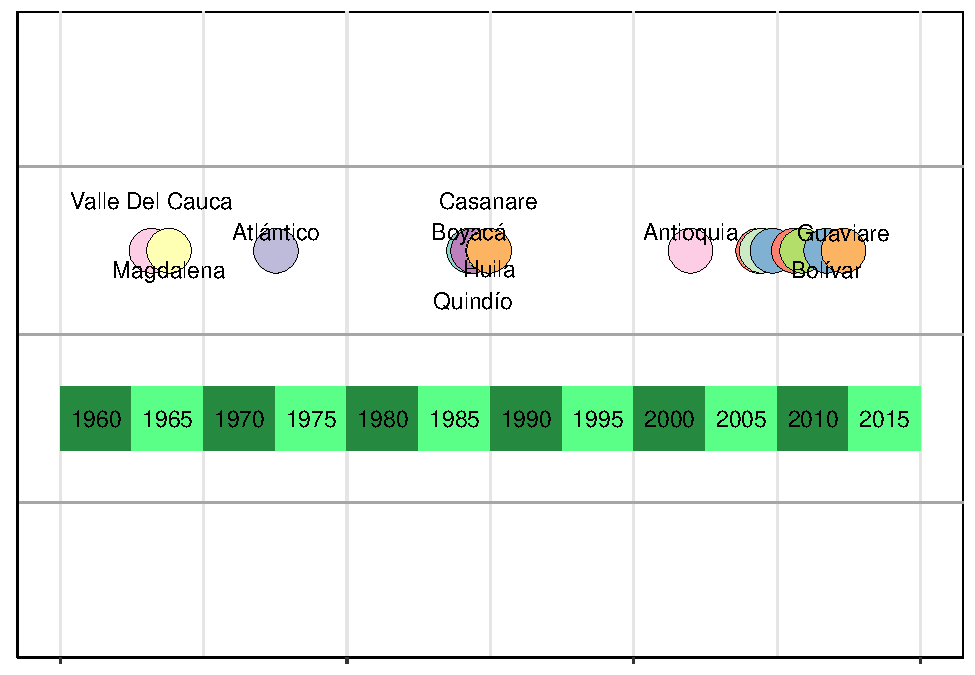
\includegraphics[width=1\linewidth,height=0.5\textheight]{InformeFinal_files/figure-latex/serieTiempoCreacion-1} 

}

\caption{Serie de tiempo de actas de creación de FRE}\label{fig:serieTiempoCreacion}
\end{figure}

Más adelante, la creación de la Federación Nacional de Departamentos (FND) permitió a los departamentos con niveles de gobernanza mucho más simples, la creación y constitución de los FRE dentro del organigrama de las respectivas entidades del nivel departamental con funciones en salud. La autonomía administrativa, financiera y presupuestal de las entidades territoriales, el respeto a la pluralidad ideológica, la promoción del desarrollo integral y el respeto a la Constitución Política y a las leyes, son los principios de la FND. Además, las asesorías en las áreas jurídica, económica, financiera y administrativa, a cargo de la FND, facultaron a los departamentos con capacidades inferiores para la constitución de sus FRE. En este periodo de tiempo se logran ver distintos FRE creados, a partir de la fecha de creación de la Federación Nacional de Departamentos (FND) en 1994\textsuperscript{\protect\hyperlink{ref-FederacionNacionaldeDepartamentos2021}{3}}.

Sin embargo, también hay algunos territorios considerados ``grandes'', debido a su situación demográfica y desarrollo económico, cuyos FRE fueron creados en la primera parte de los años 2000. Estos casos particulares (p.ej. Antioquia, Santander, Norte de Santander, y Nariño), posiblemente se podrían explicar en función de la organización interna de cada dirección departamental de salud. Especialmente, hasta ese tiempo, aquellos departamentos mostraron un interés primigenio en regular la venta de estos productos en su territorio.

Particularmente en algunos territorios del país, no se cuenta con un FRE propiamente constituido, por medio de acto administrativo, suscrito por el gobernador. Por lo tanto, el control que se tiene sobre los medicamentos denominados Monopolio del Estado, lo ejercen a partir de su propia interpretación de la Resolución 1478 del 2006\textsuperscript{\protect\hyperlink{ref-MSPS1478-2006}{4}} y Resolución 1479 del 2006\textsuperscript{\protect\hyperlink{ref-MSPS1479-2006}{1}}. Durante las asistencias técnicas desarrolladas, se presentaron algunos casos como Córdoba y Vaupés en los cuales no fue posibles verificar el acto administrativo de creación.

\hypertarget{estructura-organizacional}{%
\section{Estructura organizacional}\label{estructura-organizacional}}

La estructura organizacional de los FRE departamentales es un elemento crítico para evaluar las condiciones y características actuales de cada ente territorial, en virtud de su capacidad para cumplir todas las funciones expuestas en el Artículo 2° de la Resolución 1479 del 2006. Por este motivo, en la Figura \ref{fig:perfilProfesionalEncargado} y \ref{fig:perfilProfesional2} se muestran los diferentes profesionales que conforman los equipos de trabajo de todos los FRE a nivel nacional.

En el panel izquierdo de la Figura \ref{fig:perfilProfesionalEncargado} se observa especialmente la distribución de los perfiles profesionales de los encargados de cada FRE departamental. Se evidencia que la mayoría de departamento cuentan con Químicos Farmacéuticos como responsables encargados de los entes territoriales. De manera similar, se observan Técnicos en Regencia en Farmacia ocupando este cargo a nivel territorial, cuyos perfiles permanecen en la misma línea profesional de trabajo, referente al conocimiento y habilidades en la gestión de los medicamentos. Lo anterior, tiene ventajas en los procesos internos del FRE, ya que permite un adecuado desarrollo de las funciones principales del ente territorial y la resolución de problemas técnicos es más probable.

Por otro lado, se evidencia un grupo de profesionales diferentes a los anteriores, pero denominados como profesionales de la salud, cuyas competencias pueden relacionarse de alguna manera con la adecuada administración y gestión de los medicamentos. Por el contrario, se deben resaltar (4) profesionales, encargados de algunos FRE, que no poseen este tipo de habilidades idóneas y apropiadas, desde su formación profesional, lo que podría resultar en dificultades técnicas para el desarrollo interno de las entidades territoriales.

Para el análisis del recurso humano de los FRE se tuvieron en cuanto dos clasificaciones:

\begin{itemize}
\item
  De acuerdo con sí la persona era la encargada del FRE o un apoyo del(a) encargado(a).
\item
  De acuerdo con la carga laboral relacionada con actividades del FRE. Se consideró como personal directo a aquel que desempeña más de un 50\% de su tiempo en actividades relacionadas al FRE y personal vinculado como aquel que desempeña menos del 50\% de su tiempo en estas actividades FRE.
\end{itemize}

\begin{figure}

{\centering 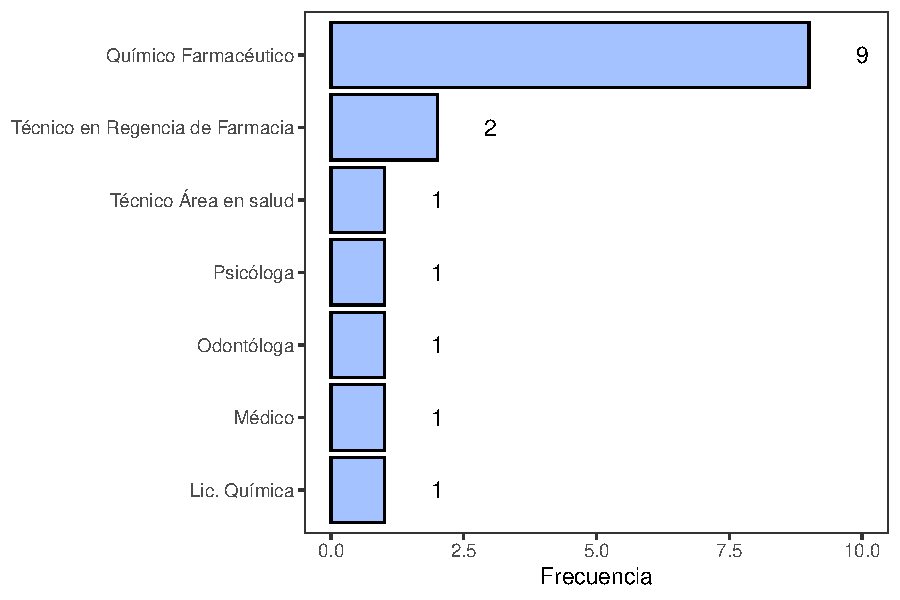
\includegraphics[width=1\linewidth]{InformeFinal_files/figure-latex/perfilProfesionalEncargado-1} 

}

\caption{Perfil de profesional de encargados de los FRE}\label{fig:perfilProfesionalEncargado}
\end{figure}

En la Figura \ref{fig:perfilProfesional2} se observan los perfiles profesionales del personal de apoyo de los FRE a nivel nacional. Principalmente, se destaca una gran mayoría de Técnicos en Regencia en Farmacia (39) seguido de un grupo menor de profesionales Químicos Farmacéuticos (10), apoyando en las actividades de los FRE departamentales. Esto demuestra que gran parte de los entes territoriales están alineados con lo expuesto en el Artículo 3° de la Resolución 1479 del 2006\textsuperscript{\protect\hyperlink{ref-MSPS1479-2006}{1}}, donde mencionan que el Químicos Farmacéuticos y Tecnólogos en Regencia en Farmacia son profesionales considerados como personal calificado para el cumplimiento de las funciones requeridas por el FRE.

\begin{figure}

{\centering 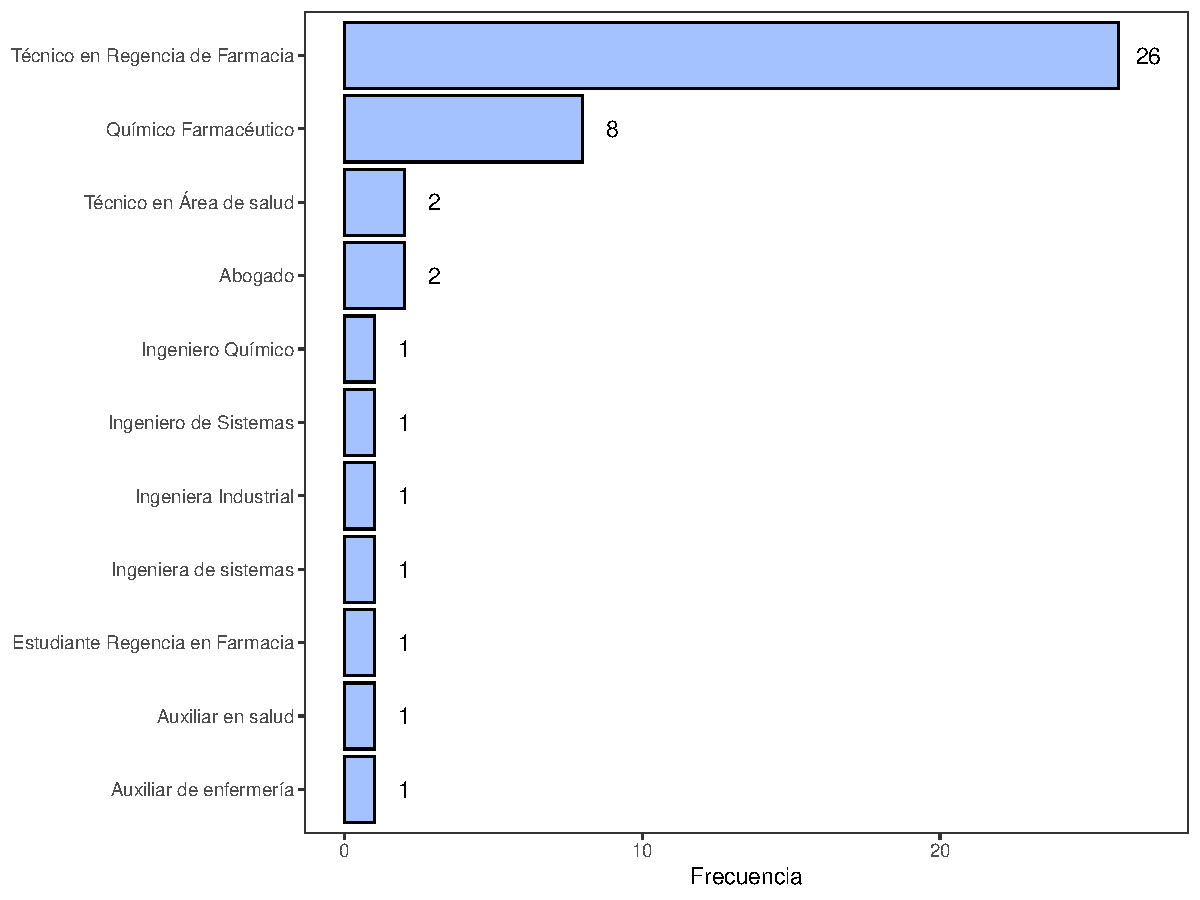
\includegraphics[width=0.9\linewidth]{InformeFinal_files/figure-latex/perfilProfesional2-1} 

}

\caption{Perfil de profesional de personal de apoyo a los FRE}\label{fig:perfilProfesional2}
\end{figure}

Adicionalmente, la Figura \ref{fig:perfilProfesional2} también muestra otro tipo de profesionales de apoyo al encargado del FRE, diferente al personal calificado mencionado anteriormente. Este factor podría brindar ventajas al equipo de trabajo del FRE particularmente, en función de la multidisciplinariedad. La participación de distintas disciplinas puede entregar más conocimientos y alternativas en el desarrollo laboral interno de cada FRE departamental. No obstante, es importante aclarar que ningún FRE debería dejar de contar con la participación del personal calificado, estipulado en el Artículo 3° de la Resolución 1479 del 2006\textsuperscript{\protect\hyperlink{ref-MSPS1479-2006}{1}}.

El número de personas que trabajan en cada FRE, es otro elemento crítico para la evaluación de condiciones y características actuales de cada ente territorial, en virtud de su capacidad para cumplir todas las funciones expuestas en el Artículo 2° de la Resolución 1479 del 2006\textsuperscript{\protect\hyperlink{ref-MSPS1479-2006}{1}}. La Figura \ref{fig:perfilProfesional3} exhibe la frecuencia absoluta del número de personas que se encuentran vinculadas a los entes territoriales del país. Es decir, la cantidad de profesionales que conforman los equipos de trabajo de todos los FRE departamentales.

\begin{figure}

{\centering 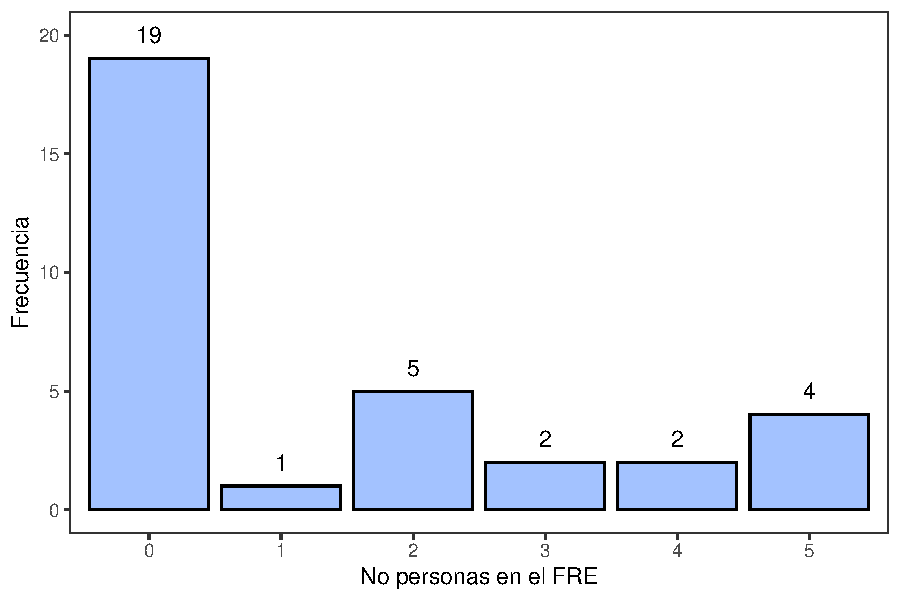
\includegraphics[width=1\linewidth]{InformeFinal_files/figure-latex/perfilProfesional3-1} 

}

\caption{N.° de personas que trabajan en el FRE}\label{fig:perfilProfesional3}
\end{figure}

Según lo anterior, podemos evidenciar que no son muchas personas vinculadas a los FRE para conformar su equipo de trabajo. En su gran mayoría tienen únicamente hasta tres personas para el desempeño del FRE, contemplando que nueve FRE tienen solo 2 personas vinculadas. Son muy pocos entes territoriales que mantienen un grupo de trabajo grande con profesionales interdisciplinarios. La Figura \ref{fig:perfilProfesional3} exhibe de manera completa los datos que acompañan el análisis anterior.

El tipo de contrato que los diferentes entes territoriales emplean para vincular el personal es otro factor crítico en el cumplimiento de las funciones de los FRE. De acuerdo con lo anterior, la Figura \ref{fig:pieProfesional2} muestra la proporción del tipo de vinculación del personal del FRE a nivel nacional, diferenciándose entre personal directo y personal vinculado. Este último, tiene cierta exclusividad con el FRE al destinar más del 50\% en actividades de este, y de acuerdo a sus obligaciones contractuales, también adelanta otras actividades con otras dependencias de la dirección departamental de salud.

A partir de la Figura \ref{fig:pieProfesional2} se puede notar una gran tendencia que tienen todos los FRE a nivel nacional, referente al tipo de vinculación por medio de Contrato Por Prestación De Servicios (CPS). La gran mayoría, precisamente, el 98\%, del personal de apoyo de los FRE está relacionado con contratos CPS. Estas personas son vinculadas al ente territorial para cumplir algunas actividades internas del FRE, pero también tienen otras actividades laborales, fuera del FRE, según sus obligaciones contractuales. Por el contrario, el personal directo al funcionamiento del FRE, cuya atención es completa en las labores internas del FRE, está relacionado en su mayoría, por nombramiento, es decir, como servidor público. En muchos departamentos, la persona encargada del FRE es el único profesional nombrado, mientras que el resto del equipo de trabajo del FRE, guardan una predisposición para ser relacionados como contratistas, por medio de CPS.

\begin{figure}

{\centering 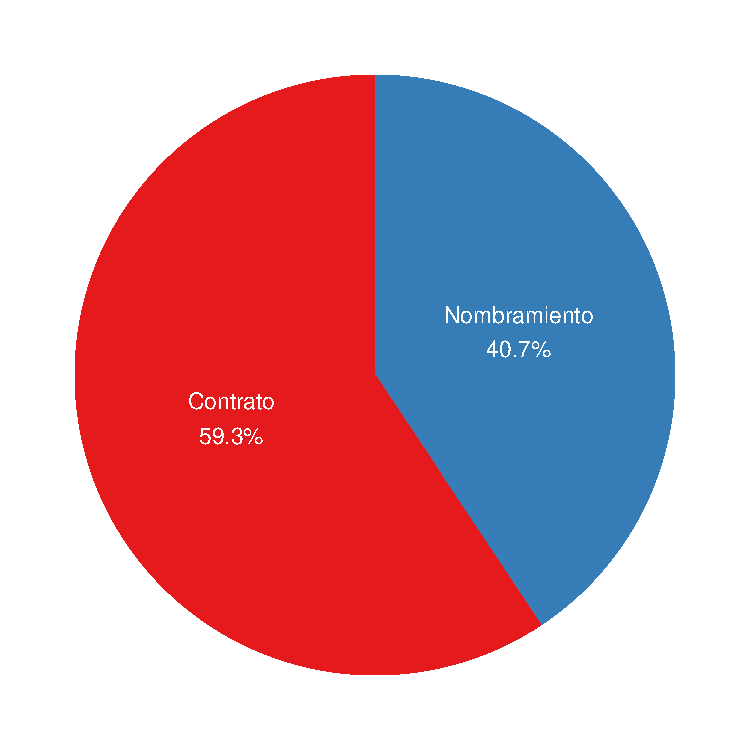
\includegraphics[width=0.85\linewidth]{InformeFinal_files/figure-latex/pieProfesional2-1} 

}

\caption{Tipo de vinculación al FRE}\label{fig:pieProfesional2}
\end{figure}

La anterior tendencia puede interferir y generar inconvenientes en la continuidad del desarrollo adecuado del FRE, afectando la funcionalidad y abandonando algunas actividades críticas para el cumplimiento de sus objetivos de creación. En algunos casos, este tipo de personas vinculadas por CPS, dejan de laborar los primeros meses del año, ya que su contrato finalizó el año pasado, y debido a barreras administrativas, no son contratadas hasta el segundo bimestre del año. El personal nombrado en muchos casos es la persona encargada del FRE, cuyos temas operativos no están dentro de su cotidianidad y no son fáciles cumplirlos. Por tal motivo estas actividades operativas se dejan de hacer en el territorio hasta que sea contratado el personal de apoyo. Como es el caso de la consolidación de los informes que deben ser enviados mensualmente al FNE.

Adicionalmente, en la Tabla \ref{tab:CaracterizacionIngreso1} se observa la proporción del tipo de vinculación del personal del FRE, discriminado por cada región del país. A partir de esta información, se observa que en 5 regiones predomina la Contratación por Prestación de Servicios respecto al Nombramiento del personal del FRE. Además, se logra observar que en las regiones más alejadas de la capital Bogotá D.C., existe una prevalencia mucho más fuerte con esta CPS. Por consiguiente, los problemas mencionados anteriormente relacionados con la CPS, se pueden notar con mayor evidencia en estos territorios apartados del centro del país.

\begin{table}

\caption{\label{tab:CaracterizacionIngreso1}Proporción de personas contratadas por región}
\centering
\begin{tabular}[t]{lll}
\toprule
Región & Nombramiento & Contratación\\
\midrule
Amazonía & 21.43\% & 78.57\%\\
Caribe & 42.86\% & 57.14\%\\
Central & 41.38\% & 58.62\%\\
Eje Cafetero & 58.33\% & 41.67\%\\
Orinoquía & 45.45\% & 54.55\%\\
\addlinespace
Pacífico & 19.23\% & 80.77\%\\
\bottomrule
\end{tabular}
\end{table}

\hypertarget{instituciones-inscritas-en-el-fre}{%
\section{Instituciones inscritas en el FRE}\label{instituciones-inscritas-en-el-fre}}

El número de instituciones inscritas en los FRE de cada departamento, puede variar según las condiciones demográficas particulares en cada territorio. Lo anterior se puede ver plasmado en la siguiente Figura \ref{fig:institucionesInscritas}, donde se exhibe el número de inscritos en cada FRE departamental. A partir de esta información, se puede apreciar el ente territorial con mayor inscritos en su territorio, correspondiendo al FRE Antioquia con un total de 1054 inscritos. Luego se posiciona en segundo lugar el FRE Valle del Cauca con 570 inscritos. Particularmente, estos dos departamentos se mantienen en los primeros lugares de los departamentos más poblados en Colombia, exceptuando Bogotá D.C. y Cundinamarca, según los datos obtenidos por el DANE en el ``Censo Nacional de Población y Vivienda 2018''\textsuperscript{\protect\hyperlink{ref-DANE2021}{5}}.

\begin{figure}

{\centering 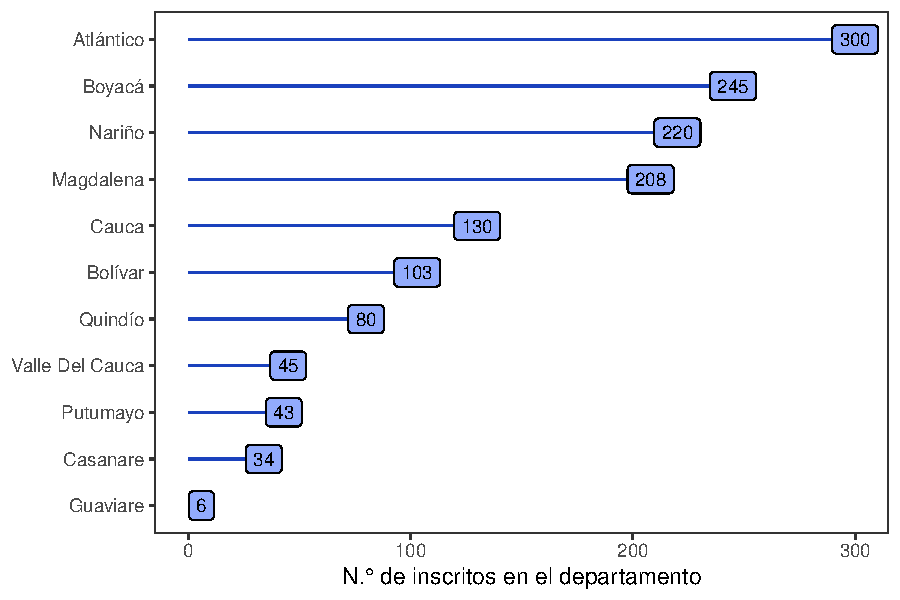
\includegraphics[width=0.9\linewidth]{InformeFinal_files/figure-latex/institucionesInscritas-1} 

}

\caption{N° de instituciones inscritas en el departamento}\label{fig:institucionesInscritas}
\end{figure}

Los FRE que continúan en la lista de mayor número de inscritos, corresponden a los entes territoriales de Norte de Santander, Santander, Atlántico y Cesar, con un rango entre 298 y 358 inscritos territorialmente. Seguidamente, se encuentran los FRE departamentales Boyacá, Caldas, Nariño y Magdalena, con un rango de instituciones inscritas territorialmente ubicado entre 208 y 245. Por otro lado, los FRE con menor número de inscritos en su territorio son los FRE departamentales Guainía, Vichada, San Andrés, Amazonas, Vaupés, Arauca y Guaviare, considerándose los departamentos de Colombia con menor población en el país, según estadísticas del DANE\textsuperscript{\protect\hyperlink{ref-DANE2021}{5}}.

Por lo tanto, se puede determinar una relación directa entre los factores demográficos de cada territorio y el número de instituciones inscritas en cada FRE. Es decir, entre menos población habite en el departamento, menos instituciones se pueden encontrar en el territorio y así mismo son menos instituciones responsables de la gestión de MME.

Existe una relación demográfica en los departamentos sobre la cantidad de instituciones inscritas y los departamentos con más densidad de población. Lo anterior se explica de acuerdo cob la capacidad del departamento para atender la necesidad de MME en su población, en función del número de personas que integran el equipo de trabajo del ente territorial. En teoría, los FRE con mayor número de inscritos, deberían estar mucho más desarrollados para atender la necesidad de MME de su población local. No obstante, en las visitas técnicas se evidenció que el recurso humano de los FRE no da abasto con todas las tareas requeridas para su funcionamiento integral.

Un claro ejemplo de estas capacidades reducidas se puede evidenciar en el desempeño de cada FRE, referente a la entrega de informes mensuales al FNE. Actualmente existen varios FRE que cuentan con un recurso humano muy amplio, pero se quedan cortos con la entrega de estos informes al FNE, como es el caso del FRE Caldas, que pese a tener una cantidad de colaboradores por encima de la media, tiene un rezago importante en la entrega de informes de consumo de medicamentos al FNE. Por consiguiente, se puede deducir que el número de personas vinculadas al FRE no comprende una garantía en el cumplimiento de todas las funciones del FRE.

También se puede observar que la distribución geográfica de las regiones no se puede relacionar con la puntualidad en el envío de informes, tomando por ejemplo el caso de la región pacífico que está compuesta por Valle del Cauca, Cauca, Chocó y Nariño. Los departamentos de Valle del Cauca y Nariño tienen una alta densidad poblacional y en la Figura \ref{fig:institucionesInscritasRelacion} también se puede observar que están respectivamente por encima y por debajo de la media en el recurso humano que tienen para su funcionamiento y son quienes envían informes de manera puntual al FNE, mientras que el departamento del Cauca supera en recurso humano a Nariño por más del doble de personal y existe un importante atraso en el envío de estos informes, posiblemente sean factores externos cómo los tipos de contratación u otras responsabilidades adquiridas por parte de los coordinadores de los FRE en su territorio.

\begin{figure}

{\centering 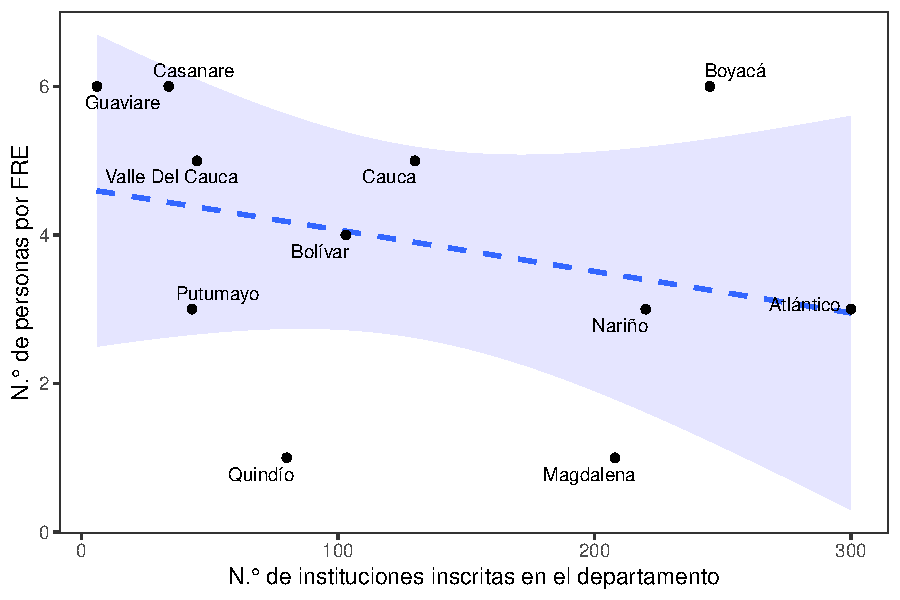
\includegraphics[width=0.85\linewidth]{InformeFinal_files/figure-latex/institucionesInscritasRelacion-1} 

}

\caption{Relación entre N° de instituciones inscritas y personal del FRE}\label{fig:institucionesInscritasRelacion}
\end{figure}

\begin{figure}

{\centering 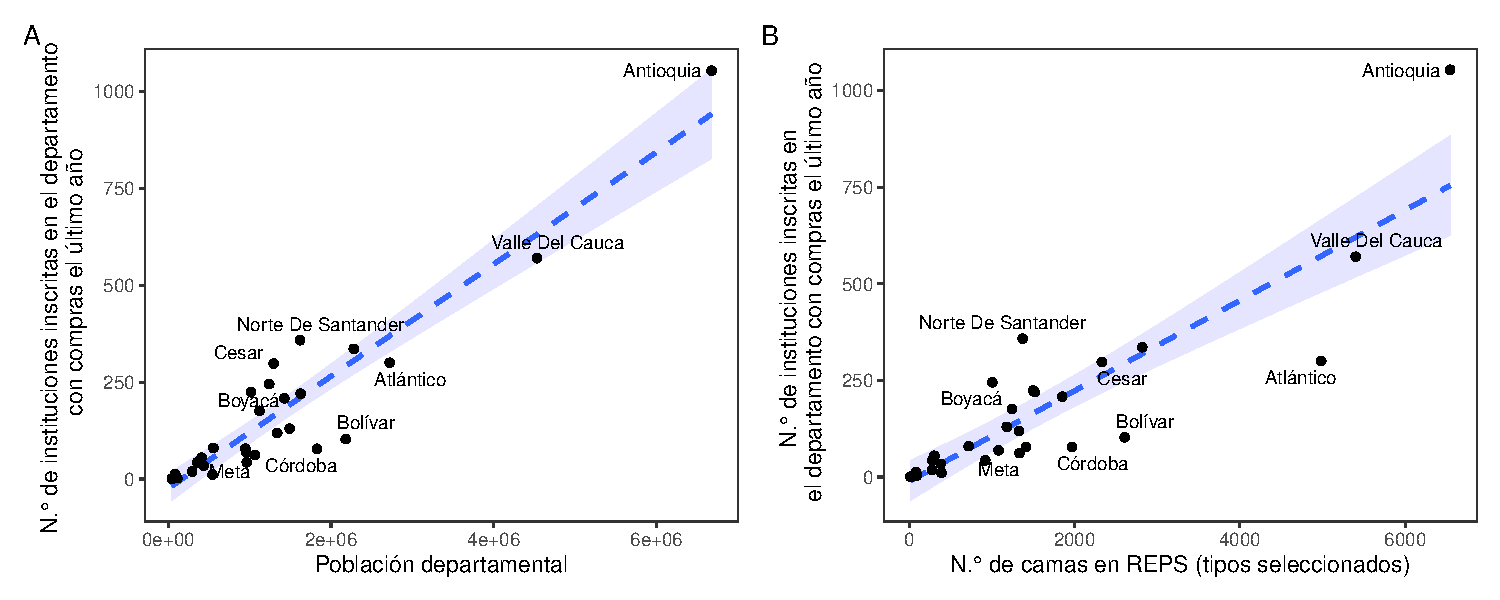
\includegraphics[width=1\linewidth]{InformeFinal_files/figure-latex/institucionesInscritasVARdemo-1} 

}

\caption{Relación entre N° de instituciones inscritas y tamaño poblacional del departamento y número de camas de acuerdo a REP}\label{fig:institucionesInscritasVARdemo}
\end{figure}

\hypertarget{caracterizaciuxf3n-de-las-fuentes-de-ingresos-de-los-fre}{%
\section{Caracterización de las fuentes de ingresos de los FRE}\label{caracterizaciuxf3n-de-las-fuentes-de-ingresos-de-los-fre}}

Para analizar las fuentes de ingreso que poseen los diferentes FRE departamentales, se debe tener en cuenta la posición del FRE dentro del organigrama de cada dirección departamental en salud. El análisis de las fuentes de ingresos de los FRE, en este punto, se hará exclusivamente con la información recolectada a partir del instrumento de encuesta que se usó para la recolección de información pertinente en este informe.

Cómo antecedente en el análisis, se entiende según las definiciones de la Resolución 1478 del 2006\textsuperscript{\protect\hyperlink{ref-MSPS1478-2006}{4}}, que un Fondo Rotatorio de Estupefacientes es:

\begin{quote}
\emph{``La Oficina encargada dentro de la Secretaría, Instituto o Dirección de Salud a nivel departamental, que ejerce la vigilancia, seguimiento y control a las entidades públicas, privadas y personas naturales que procesen, manipulen, sinteticen, fabriquen, distribuyan, vendan, consuman, dispensen sustancias sometidas a fiscalización y medicamentos que las contengan; así como garantizar la disponibilidad de medicamentos Monopolio del Estado a través de la dispensación y distribución en su jurisdicción y las demás funciones que le sean asignadas por el Ministerio de la Protección Social, o la institución competente.''}
\end{quote}

Por lo tanto, es una dependencia del ente territorial y no goza de autonomía administrativa o financiera cómo para ser considerada una Unidad Administrativa Especial, cómo si lo es el Fondo Nacional de Estupefacientes con sede en Bogotá, sin embargo, de acuerdo al Artículo 3 de la Resolución 1479 del 2006, los FRE\textsuperscript{\protect\hyperlink{ref-MSPS1479-2006}{1}}:

\begin{quote}
\emph{``{[}\ldots{]} deben tener una cuenta específica denominada ``Fondo Rotatorio de Estupefacientes'' para manejar sus operaciones. Las utilidades que se obtengan sólo podrán emplearse, para su administración, mejoras de dotación, buen funcionamiento del mismo y ejecutar programas contra la farmacodependencia y toxicología que adelante el Gobierno Nacional.''}
\end{quote}

De modo que la normativa interna de cada departamento podría entrar en conflicto con la misma resolución anteriormente citada que define las funciones y capacidades de los FRE, pudiendo generar bloqueos o demoras en determinados procesos internos que permitan un funcionamiento integral en el manejo de los MME.

Hecho este primer paso sobre entender de manera sucinta la relación que tienen los FRE con sus respectivas entidades territoriales, se puede comenzar a hacer el análisis de las gráficas con los resultados del instrumento de encuesta realizado.

\begin{figure}

{\centering 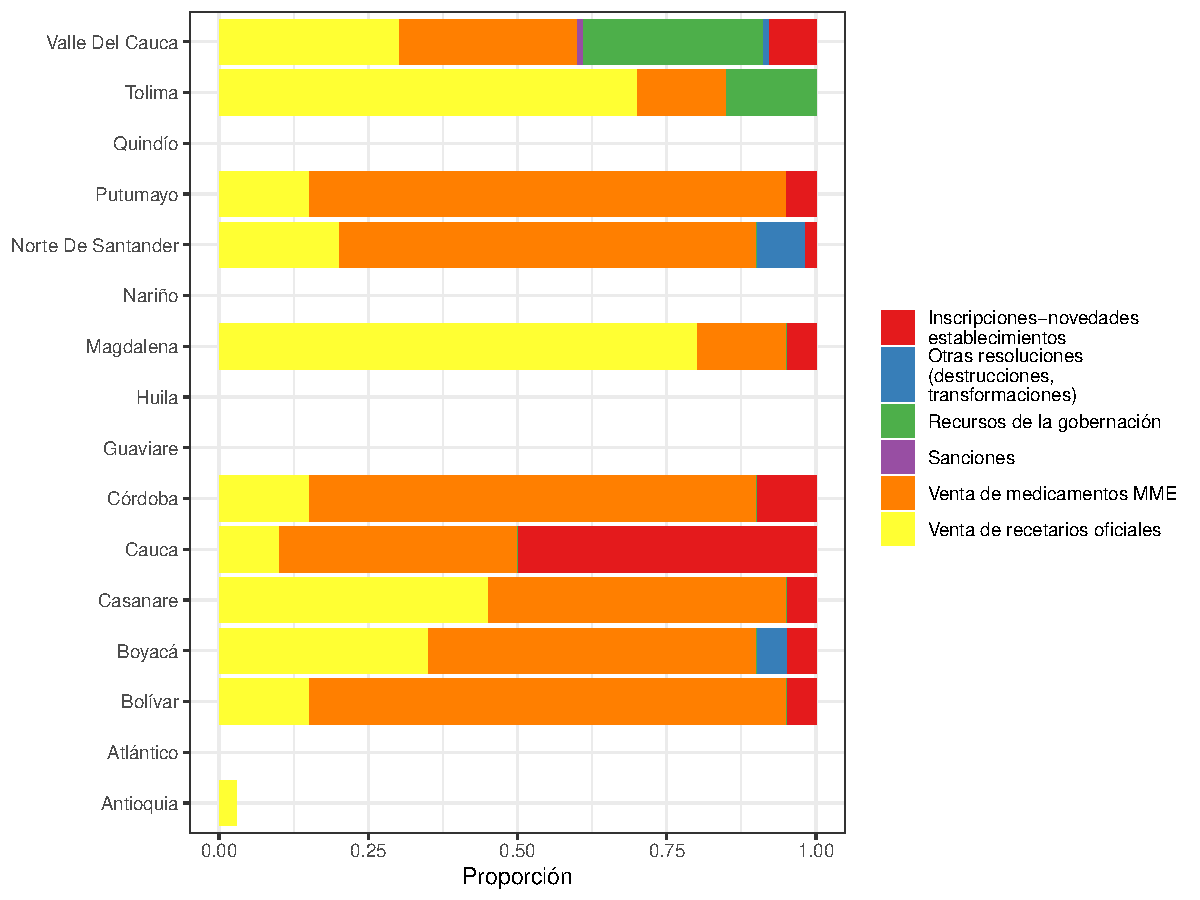
\includegraphics[width=0.85\linewidth]{InformeFinal_files/figure-latex/IngresosFRE1-1} 

}

\caption{Proporción de fuentes de ingresos de los FRE}\label{fig:IngresosFRE1}
\end{figure}

La Figura \ref{fig:IngresosFRE1}, nos muestra la proporción de los ingresos del FRE en sus cuentas bancarias, en base a las que serían sus principales actividades, cómo lo son:

\begin{itemize}
\item
  Venta de Medicamentos Monopolio del Estado
\item
  Venta de Recetarios Oficiales
\item
  Producción y emisión de actos administrativos pertinentes al manejo de MME
\item
  Inspección, Vigilancia y Control de Instituciones que manejen MCE
\end{itemize}

Aunque también los FRE pueden recibir recursos por parte de la gobernación o por parte del FNE.

A partir de la Figura \ref{fig:IngresosFRE1}, se observa que la venta de MME tiene una tendencia a ser la proporción más grande sobre los ingresos que reciben los FRE departamentales. Esto se puede deber a que cada departamento maneja independencia en los precios de venta de estos medicamentos y desde ahí se podría obtener una rentabilidad mayor. En el desarrollo del apartado 6.4 Precio de medicamentos del presente informe, se desglosará un análisis más profundo sobre los precios de venta de los MME por departamento, pero grosso modo se puede notar que el margen es lo suficientemente alto para abarcar el porcentaje mayoritario de ingresos.

Particularmente, en la Figura \ref{fig:IngresosFRE2} se observa que en algunos departamentos cómo Magdalena, Atlántico o Tolima, la venta de recetarios oficiales es el ingreso más prominente del FRE. Así mismo, en todos los demás departamentos representa un ingreso importante para el ente territorial, aunque no sea la principal fuente de ingreso. A nivel nacional, esta fuente de ingreso carga con una parte muy importante del erario de cada FRE departamental. Con la desaparición de los recetarios oficiales físicos en el mediano plazo, es necesario generar alternativas económicas para subsanar este recurso que desaparecería y adecuar estrategias financieras para el auto sostenimiento de cada FRE.

\begin{figure}

{\centering 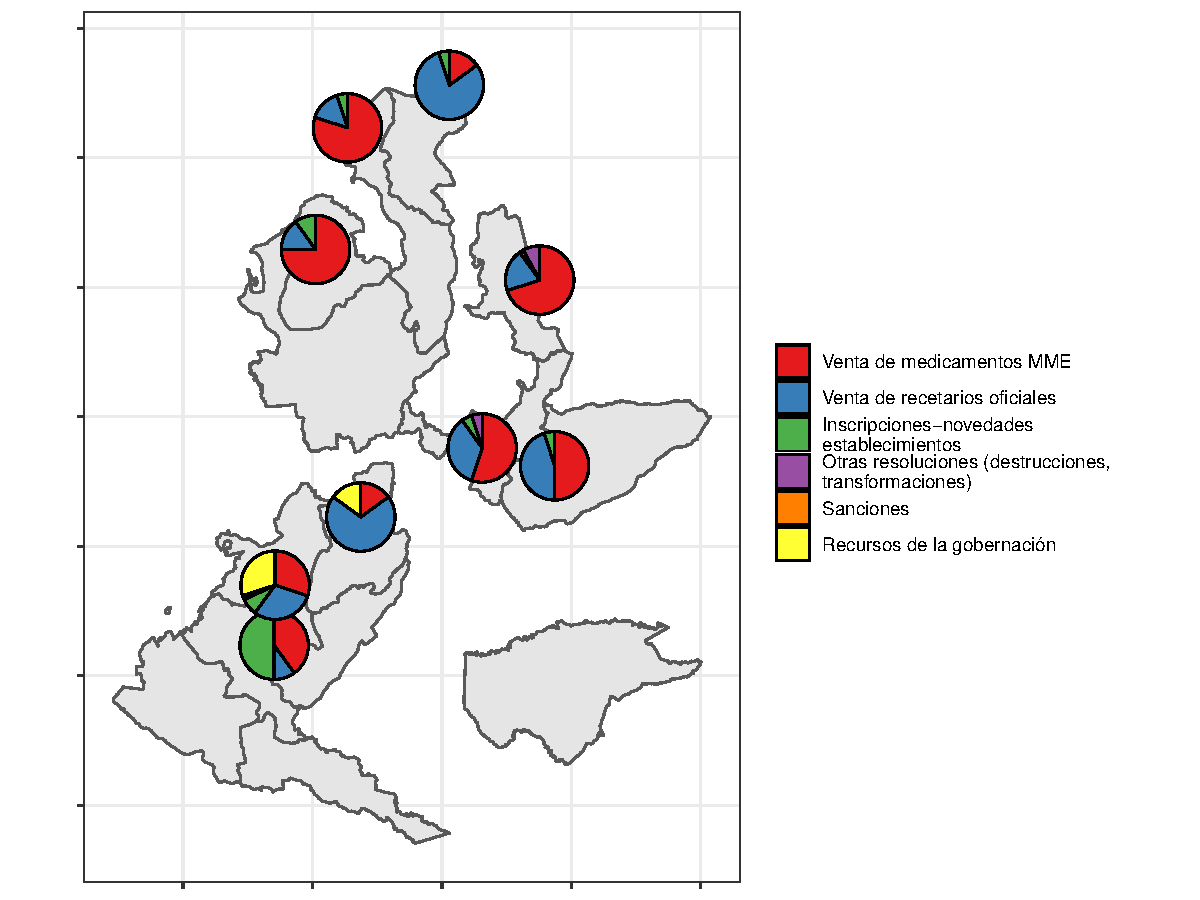
\includegraphics[width=0.85\linewidth]{InformeFinal_files/figure-latex/IngresosFRE2-1} 

}

\caption{Mapa con fuentes de ingresos de los FRE}\label{fig:IngresosFRE2}
\end{figure}

\textbf{En algunos casos no se logró obtener información de las fuentes de información\ldots{}}

\hypertarget{recetarios-oficiales}{%
\chapter{Recetarios oficiales}\label{recetarios-oficiales}}

\maxdeadcycles=1000

El recetario oficial es un documento oficial avalado por la entidad competente, es de carácter personal e intransferible para uso de los prescriptores de salud en la formulación de los medicamentos de control especial y de Monopolio del Estado. La prescripción de medicamentos de control especial para uso humano o veterinario solo se podrá efectuar en los recetarios oficiales suministrados por los FRE, para médicos en ejercicio legal de su profesión y/o por el Consejo Profesional de Medicina Veterinaria y Zootecnia de Colombia (Comvezcol) para médicos veterinarios y médicos veterinarios zootecnistas. Los profesionales que laboren en las instituciones podrán hacer uso del Recetario Oficial adquirido por la entidad\textsuperscript{\protect\hyperlink{ref-MSPS1478-2006}{4}}.

Los FRE de las Secretarías, Instituciones o Direcciones Departamentales de Salud, y/o Comvezcol para médicos veterinarios, son los únicos autorizados para emitir, distribuir y vender el Recetario Oficial para la prescripción\textsuperscript{\protect\hyperlink{ref-MSPS1478-2006}{4}}.

\hypertarget{existencia-de-recetarios}{%
\section{Existencia de recetarios}\label{existencia-de-recetarios}}

\hypertarget{existencias-en-el-fre}{%
\subsection{Existencias en el FRE}\label{existencias-en-el-fre}}

En el marco de las Jornadas de inmersión territoriales con los FRE del país se pudo determinar la cantidad de recetarios oficiales con los que cuentan entre los meses de junio a septiembre. Así pues, como se observa en la Figura \ref{fig:existenciasRecetarios}A, se observa la tendencia de los departamentos más distantes de la capital de la nación, a presentar una menor cantidad de recetarios en existencia.

\begin{figure}

{\centering 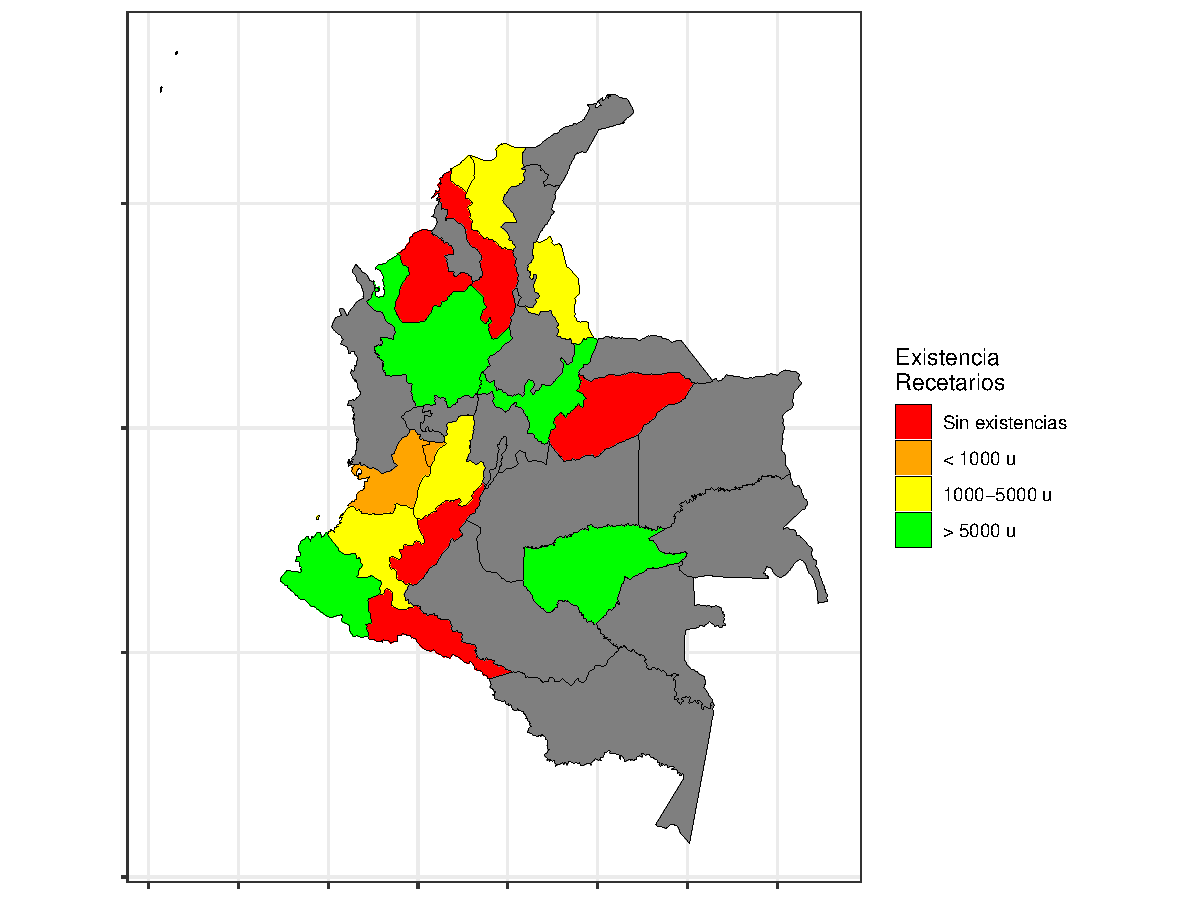
\includegraphics[width=1\linewidth]{InformeFinal_files/figure-latex/existenciasRecetarios-1} 

}

\caption{Existencias en el FRE. Panel A. N.° de existencias de recetarios en el FRE. Panel B. Cobertura de existencias de recetarios en el FRE.}\label{fig:existenciasRecetarios}
\end{figure}

En los extremos norte y sur, es decir, la región Caribe y Amazónica se tiene la mayor proporción de inexistencias de recetarios, en comparación con el resto de las regiones. El motivo de esto puede ser la dificultad para encontrar empresas de fabricación adecuada de documentos con características particulares como lo son los recetarios oficiales, por los cuales, en algunos departamentos limítrofes se contratan empresas de departamentos del interior, dado que en sus regiones no existe la capacidad para elaborarlos. Por otro lado, los FRE más antiguos y consolidados son los que en el presente disponen de mayor cantidad de recetarios, lo que puede estar influenciado, igualmente por la cercanía y facilidad de contratación con empresas de la región.

Dentro del censo realizado en los diferentes departamentos del país, se observa en la Figura \ref{fig:existenciasRecetarios}B predisposición entre los distintos FRE a presentar en estos momentos una duración de existencias de recetarios oficiales a 25 semanas. El motivo de esto es que en gran parte de los entes territoriales se concretan órdenes de compra de recetarios por un año, de modo que en la época en la cual se realizó el censo, aproximadamente mitad de año, aún quedan alrededor de 20 a 30 semanas más para la finalización del año calendario. Además de ello, en ocasiones se estima un periodo de 2 a 3 meses más, es decir, disponibilidad de recetarios hasta febrero o marzo, ya que por motivos de contratación de personal a inicio del año calendario se dificulta llevar a cabo el proceso de licitación de recetarios hasta que se hayan contratado nuevamente a los funcionarios del FRE, cuestión que se da por el tipo de contrato laboral con el que están vinculados la mayoría de los funcionarios de apoyo en el país (Figura \ref{fig:pieProfesional2}).

Se tiene que Boyacá y Nariño son los departamentos que en la actualidad cuentan con mayor proyección de disponibilidad de recetarios oficiales ya que son regiones en donde el FRE hace compras para 2 a 3 años, procesos que fueron llevados a cabo recientemente, a inicio del año 2021.

\hypertarget{circulaciuxf3n-en-el-departamento}{%
\subsection{Circulación en el departamento}\label{circulaciuxf3n-en-el-departamento}}

Así mismo, ligado a las existencias actuales de recetarios oficiales en la nación, como se observa en la Figura \ref{fig:existenciasRecetarios2}, los departamentos en donde se presenta menor circulación de recetarios precisamente son los departamentos distantes del interior. Este fenómeno puede ser ocasionado por la baja densidad poblacional de dichos territorios, es decir, la rotación de recetarios oficiales en Antioquia, que es un departamento que cuenta con más de 5 millones de habitantes es la más alta ya que su población actual supera a la de los demás departamentos que cuentan con recetarios oficiales\textsuperscript{\protect\hyperlink{ref-DANE2021}{5}}.

\begin{figure}

{\centering 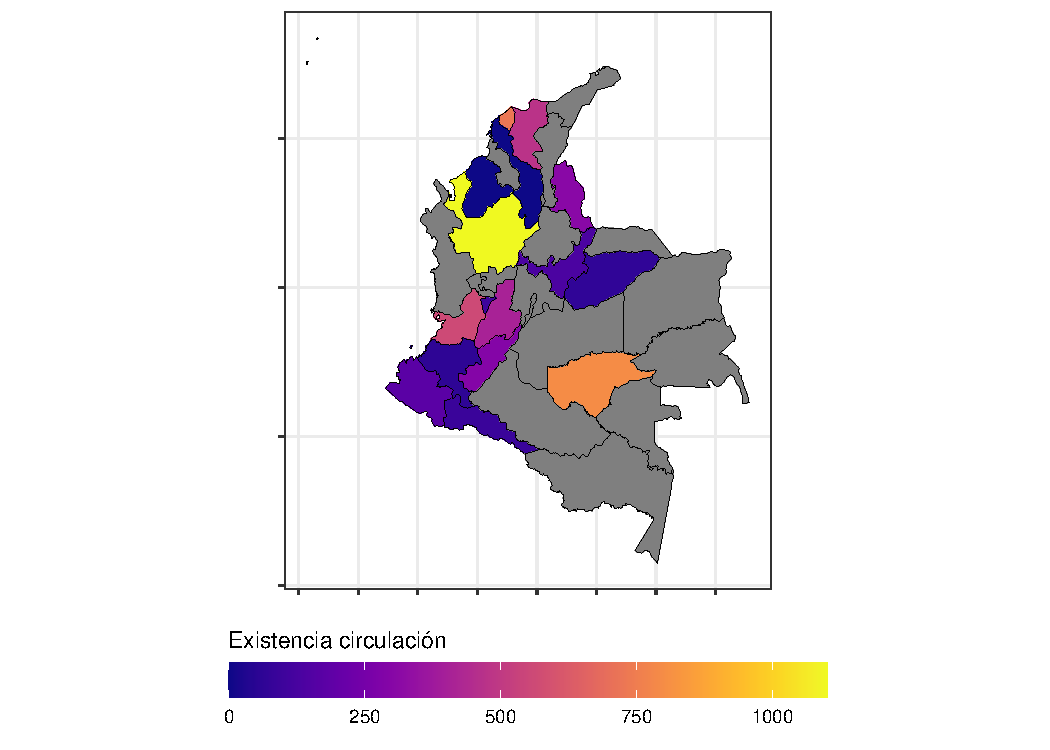
\includegraphics[width=0.85\linewidth]{InformeFinal_files/figure-latex/existenciasRecetarios2-1} 

}

\caption{N.° de recetarios circulantes en el departamento}\label{fig:existenciasRecetarios2}
\end{figure}

\hypertarget{costos-de-recetarios}{%
\section{Costos de recetarios}\label{costos-de-recetarios}}

\maxdeadcycles=1000

\hypertarget{comparaciuxf3n-de-costos-y-precios-de-ventas-de-recetarios}{%
\subsection{Comparación de costos y precios de ventas de recetarios}\label{comparaciuxf3n-de-costos-y-precios-de-ventas-de-recetarios}}

Dentro del estudio de costos realizado se comparó el costo de compra del recetario contra su precio de venta. Así pues, se determinó que dentro del territorio el costo de los recetarios ronda entre los 10.000 COP y los 20.000 COP, con territorios como Valle del Cauca y Casanare, en donde dicho costo se aproxima a 30.000 COP. En algunos departamentos no se conocen los costos de adquisición de recetarios (Figura \ref{fig:costoRecetario}A), dada sus particularidades en la contratación, puesto que se encargan del proceso de licitación y contratación de recetarios, únicamente realizan estudios de necesidad que son enviados al ente encargado de concretar la contratación, en muchos casos, la gobernación departamental.

\begin{figure}

{\centering 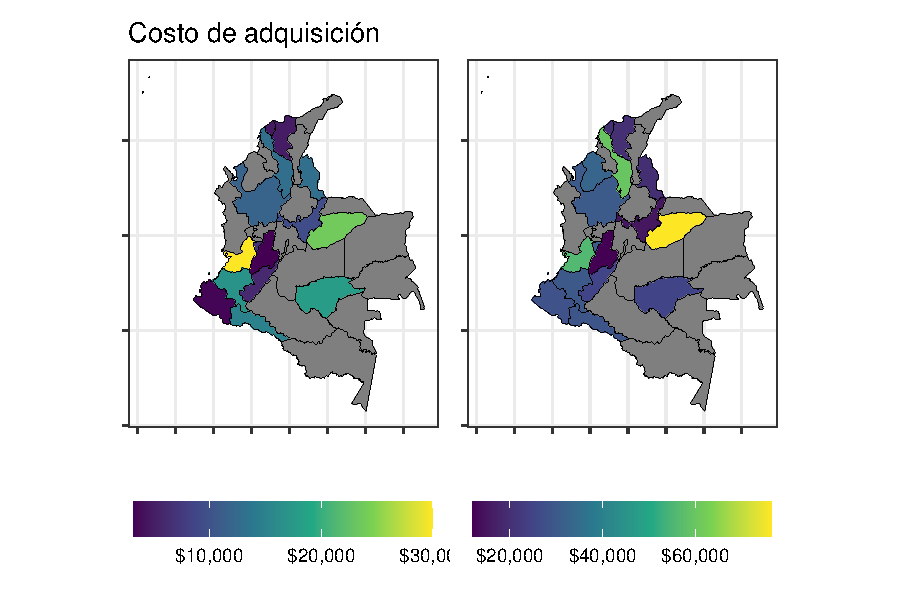
\includegraphics[width=0.9\linewidth]{InformeFinal_files/figure-latex/costoRecetario-1} 

}

\caption{Comparativo de costo vs precio de recetarios por departamento. Panel A. Costos de adquisición de recetarios por departamento. Panel B. Precios de recetarios por departamento.}\label{fig:costoRecetario}
\end{figure}

Por otro lado, el precio de venta de los recetarios tiende a rondar los 30.000 COP, ya que en algunos FRE por acto administrativo se ha establecido la tarifa del recetario con base en el salario mínimo diario legal vigente (Figura \ref{fig:costoRecetario}B) que se ajusta cada año. Así mismo, se observa correlación entre los departamentos con costo de recetario más alto y precio de venta mayor, como se da en Valle del Cauca, Bolívar y Casanare.

Ahora bien, el margen de ganancias que deja la venta de recetarios se observa en la Figura \ref{fig:comparativoDepartamentos0}, en donde se puede establecer que con mayor frecuencia los entes territoriales obtienen entre 100 y 200\% de ganancia sobre el costo del recetario. No obstante, los FRE de La Guajira y Nariño, poseen ganancias entre 800 y 900\% en la venta de sus recetarios oficiales. En los FRE de Córdoba, Vichada y Guainía no se registran márgenes de ganancia para la venta de recetarios oficiales dado que no se tiene conocimiento en dichos territorios del costo de adquisición de recetarios puesto que son los entes gubernamentales del departamento los encargados de la contratación, proceso en el que el ente territorial no interviene.

\begin{figure}

{\centering 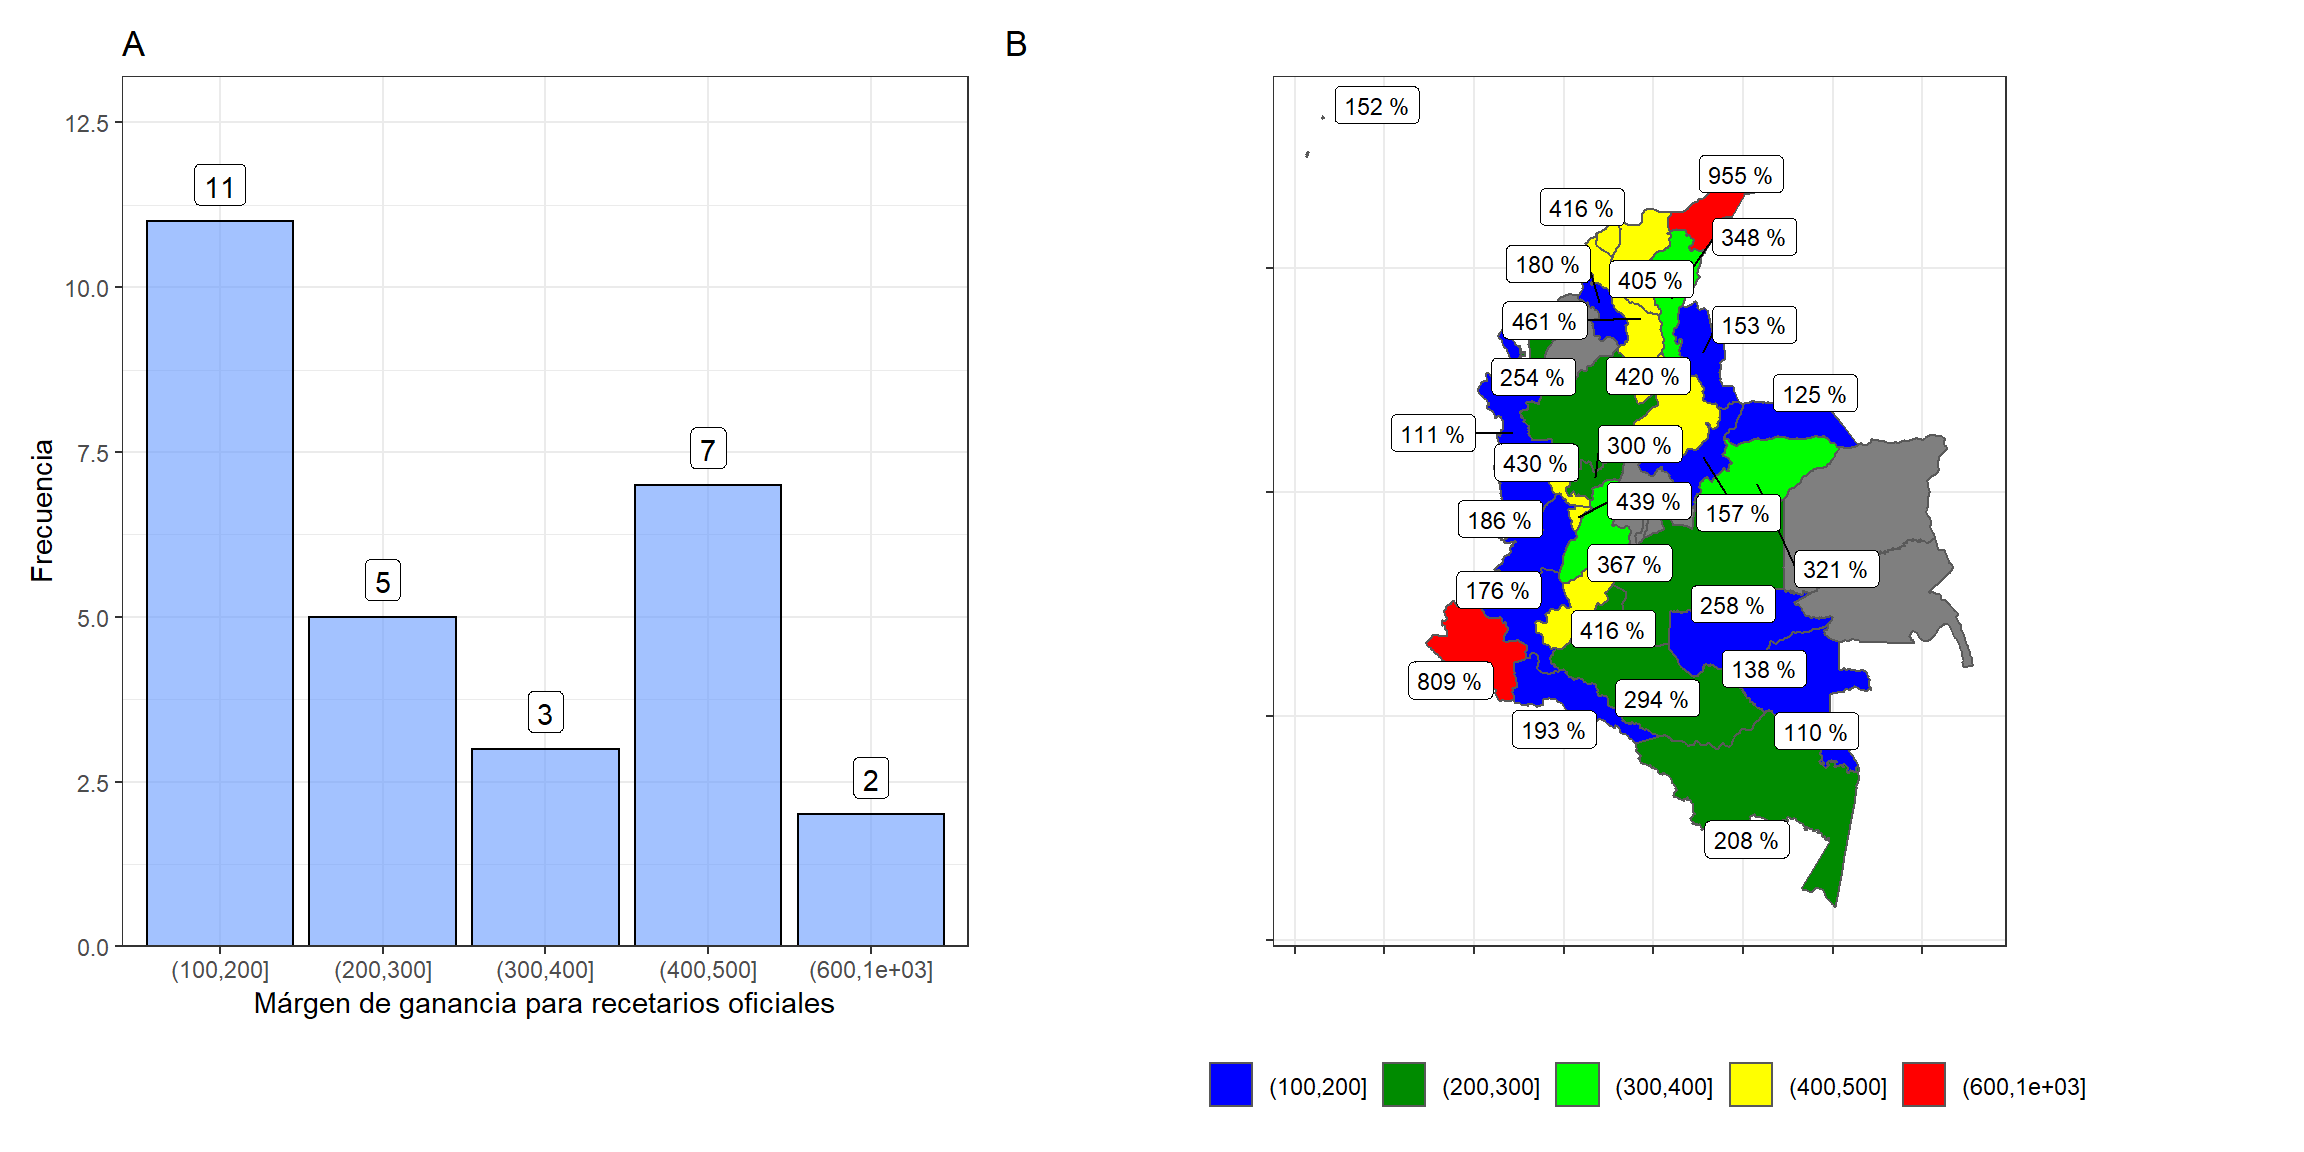
\includegraphics[width=1\linewidth]{InformeFinal_files/figure-latex/comparativoDepartamentos0-1} 

}

\caption{Márgen de ganancia por recetario. Panel A. Frecuencia de departamentos por márgen de ganancia. Panel B. Márgen de ganancia de recetarios por departamento.}\label{fig:comparativoDepartamentos0}
\end{figure}

Los amplios márgenes de ganancia y las proporciones distintas entre unos FRE y otros, se podrían relacionar con: (a) cantidad de medidas de seguridad del recetario, (b) facilidad de acceso del departamento, (c) número de prescripciones, (d) tipo de licitación o (e) cantidad de empresas oferentes en los concursos de licitación de recetarios.

\hypertarget{factores-que-afectan-el-costo-de-adquisiciuxf3n-de-recetarios}{%
\subsection{Factores que afectan el costo de adquisición de recetarios}\label{factores-que-afectan-el-costo-de-adquisiciuxf3n-de-recetarios}}

Dentro de los procesos que se utilizan para la licitación y contratación de recetarios oficiales en el país, se consideran 4 modalidades de selección principalmente:

\begin{itemize}
\item
  Licitación pública, el cual es un proceso de selección utilizado por las entidades estatales mediante el cual escoge a sus contratistas a través de una invitación de carácter público que se dirige a todas las personas potencialmente interesadas en ejecutar un contrato, para que en igualdad de condiciones y bajo criterios objetivos garantizados por el pliego de condiciones, presenten ofertas entre las que se escogerá la más favorable\textsuperscript{\protect\hyperlink{ref-MinisteriodeRelacionesExteriores2014}{6}}.
\item
  Selección abreviada, modalidad de selección objetiva prevista en aquellos casos en que por las características del objeto a contratar, las circunstancias de la contratación o la cuantía o destinación del bien, obra o servicio, puedan adelantarse procesos simplificados (uso de subastas a la inversa, bolsas de productos o compras por catálogo) para garantizar la eficacia de la gestión contractual\textsuperscript{\protect\hyperlink{ref-MinisteriodeRelacionesExteriores2014}{6}}.
\item
  Contratación directa, que es de carácter excepcional, por lo que su aplicación es de carácter restrictivo. En efecto, la ley de Contratación Pública en Colombia, prevé los siguientes eventos en los cuales es procedente esta modalidad de contratación: casos de urgencia manifiesta, contratación de empréstitos, cuando no exista pluralidad de oferentes en el mercado, para los contratos de desarrollo de actividades científicas y tecnológicas, entre otros\textsuperscript{\protect\hyperlink{ref-MinisteriodeRelacionesExteriores2014}{6}}.
\item
  Mínima cuantía, que es un procedimiento sencillo y rápido para escoger al contratista en la adquisición de los bienes, obras y servicios cuyo valor no exceda el diez por ciento (10\%) de la menor cuantía de las Entidades Estatales, modalidad de selección que tiene menos formalidades que las demás\textsuperscript{\protect\hyperlink{ref-ColombiaCompraEficiente2019}{7}}.
\end{itemize}

Se realizó una exploración de los factores que pueden afectar el costo de los recetarios mediante un análisis de regresión lineal múltiple, para lo cual se tomó el costo de los recetarios, y se tuvieron en cuenta regresores como:

\begin{itemize}
\item
  número de prescripciones en el recetario (variable continua).
\item
  número de medidas de seguridad implementadas en el recetario (variable continua).
\item
  modalidad de selección de oferentes en la contratación (variable categórica con cuatro niveles mencionadas previamente)
\end{itemize}

\begin{table}

\caption{\label{tab:resumenModeloRegresionLineal}Resumen de modelo de regresión lineal múltiple para el costo del recetario.}
\centering
\begin{tabular}[t]{lcccc}
\toprule
Parámetro & Estimado & Error Estándar & Valor t & Pr(>|t|)\\
\midrule
Intercepto & 12181.9 & 12799.4 & 0.952 & 0.352\\
N.° de prescripciones & 228.1 & 177.8 & 1.283 & 0.213\\
N.° de medidas & -1712.0 & 1578.6 & -1.085 & 0.290\\
Modalidad - Licitación pública & -4760.7 & 12064.4 & -0.395 & 0.697\\
Modalidad - Mínima Cuantía & -3656.2 & 8269.9 & -0.442 & 0.663\\
\addlinespace
Modalidad - Selección abreviada & -1414.0 & 14418.9 & -0.098 & 0.923\\
\bottomrule
\end{tabular}
\end{table}

El modelo generado (ver Tabla \ref{tab:resumenModeloRegresionLineal}) presenta una bondad de ajuste muy baja (\(R^{2} = -0.064\)), y no se logra demostrar un efecto significativo de los factores explorados, pese a esto se presentan tendencias en estos factores.

En la Figura \ref{fig:DependParcial1} se muestran gráficos de dependencia parcial de los factores explorados, se observan tendencias como que el N.° de prescripciones elevan el costo de los recetarios. Pese a que se podría suponer que al aumentar el número de características de seguridad en el recetario se aumentaría el costo de este, se encuentra una relación inversa entre el número de medidas y el costo de adquisición. Esto podría deberse a la facilidad de elaboración en departamentos con la capacidad tecnológica adecuada, la forma en que se adjudican los contratos y los diferentes oferentes en el concurso de contratación.

\begin{figure}

{\centering 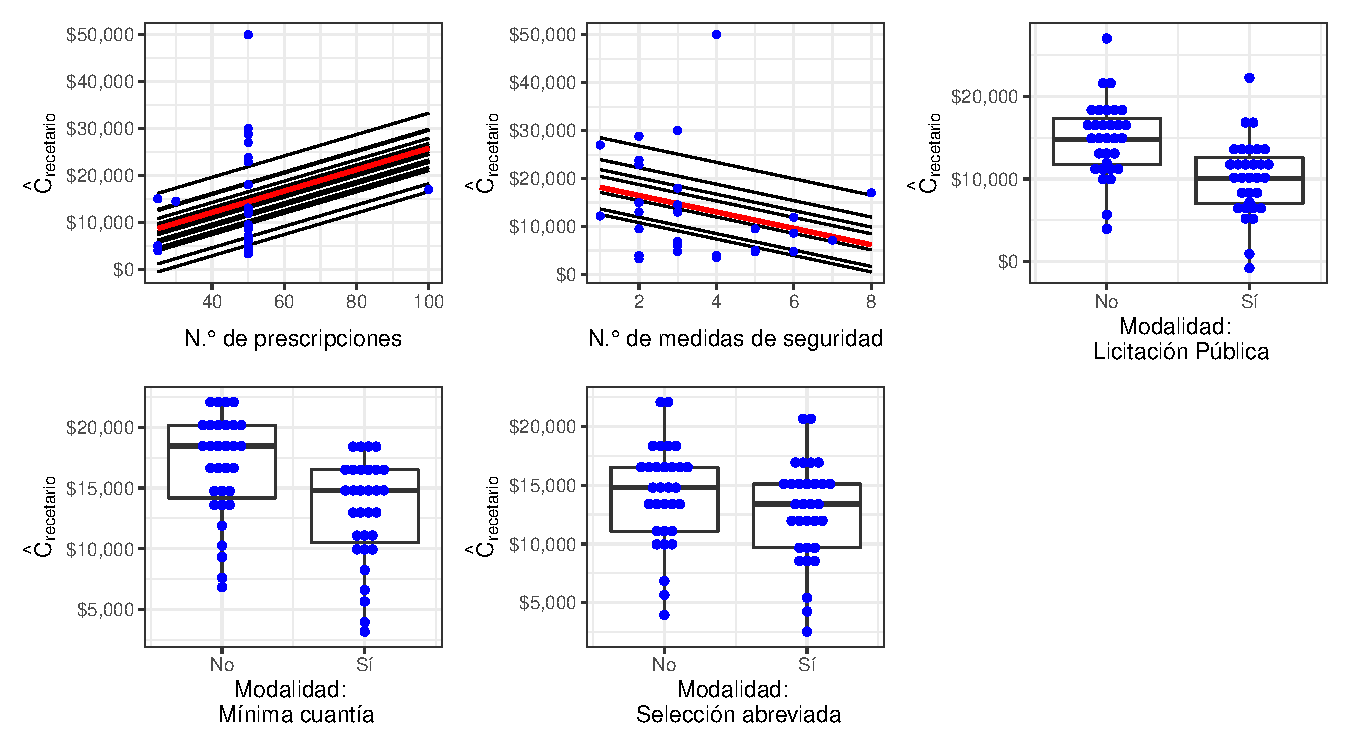
\includegraphics[width=0.9\linewidth]{InformeFinal_files/figure-latex/DependParcial1-1} 

}

\caption{Gráficos de dependencia parcial - Modelo de Costos.}\label{fig:DependParcial1}
\end{figure}

De esta forma, el tipo de contratación que se concreta con las empresas fabricante de los recetarios es una variable que influye en el costo de los recetarios, así pues, las modalidades de contratación por licitación pública, mínima cuantía y selección abreviada tienden a disminuir el costo del recetario en comparación con la modalidad de contratación directa, factor esperado ya que al no haber competencia entre empresas oferentes, quien posee el monopolio de fabricación es libre de disponer los precios de venta a las entidades territoriales.

Por otra parte, los FRE que concretaron órdenes de compra de recetarios por mínima cuantía y selección abreviada, tienden a presentar precios mayores de adquisición, con costo alrededor de los 10.000 COP y 15.000 COP, mientras que, los entes territoriales que optaron por la modalidad de licitación pública tienden a ser los recetarios más económicos en relación con las demás, con costos inferiores a los 10.000 COP por recetario en promedio.

\hypertarget{precio-de-venta-de-recetario-por-prescripciuxf3n}{%
\subsection{Precio de venta de recetario por prescripción}\label{precio-de-venta-de-recetario-por-prescripciuxf3n}}

Finalmente, se concluye que el precio por prescripción de los recetarios oficiales circulantes a nivel nacional como variante ponderadora el precio de venta y la cantidad de prescripciones por recetario, en donde se puede evidenciar la tendencia de los FRE hacia 250 COP a 500 COP por prescripción (Figura \ref{fig:PVTA-Recetarios}).

\begin{figure}

{\centering 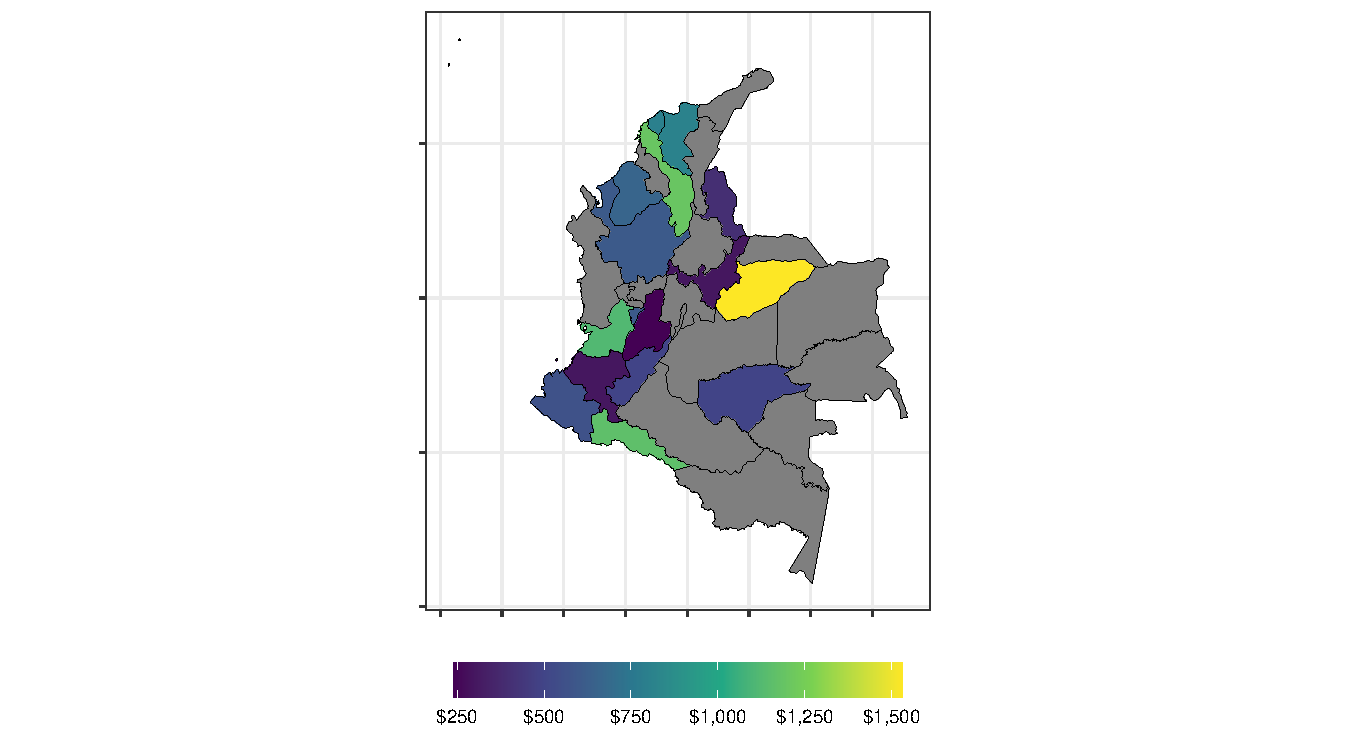
\includegraphics[width=0.9\linewidth]{InformeFinal_files/figure-latex/PVTA-Recetarios-1} 

}

\caption{Precio de venta de recetario por prescripción.}\label{fig:PVTA-Recetarios}
\end{figure}

El valor por prescripción más alto a nivel nacional se presenta en el departamento de Casanare, pese a que este recetario cuenta con 50 prescripciones como la mayoría de los FRE, su precio de venta es de 76.500 COP, el más alto del país, y del que no se tiene un acto administrativo donde se establezca su valor. Además de ello, cuenta con 3 medidas de seguridad, lo que consolida la hipótesis que se observa a nivel nacional que indica que, a menor número de medidas de seguridad, mayor es el costo del recetario.

El precio de venta por prescripción podría incrementar los costos a los que se venden los MME a los pacientes en los puntos de dispensación.

\hypertarget{adquisiciuxf3n-de-recetarios}{%
\section{Adquisición de recetarios}\label{adquisiciuxf3n-de-recetarios}}

\maxdeadcycles=1000

\hypertarget{proceso-de-adquisiciuxf3n-de-recetario}{%
\subsection{Proceso de adquisición de recetario}\label{proceso-de-adquisiciuxf3n-de-recetario}}

La adquisición de recetarios oficiales por parte de los FRE es un proceso que se lleva a cabe mediante contratación pública. En la Figura \ref{fig:modalidadAdquisicion}, se muestra un resumen de las modalidades de selección en el último proceso de adquisición de recetarios por parte de los FRE. Se evidencia que la modalidad más utilizada en este último periodo de reabastecimiento de recetario fue mínima cuantía.

\begin{figure}

{\centering 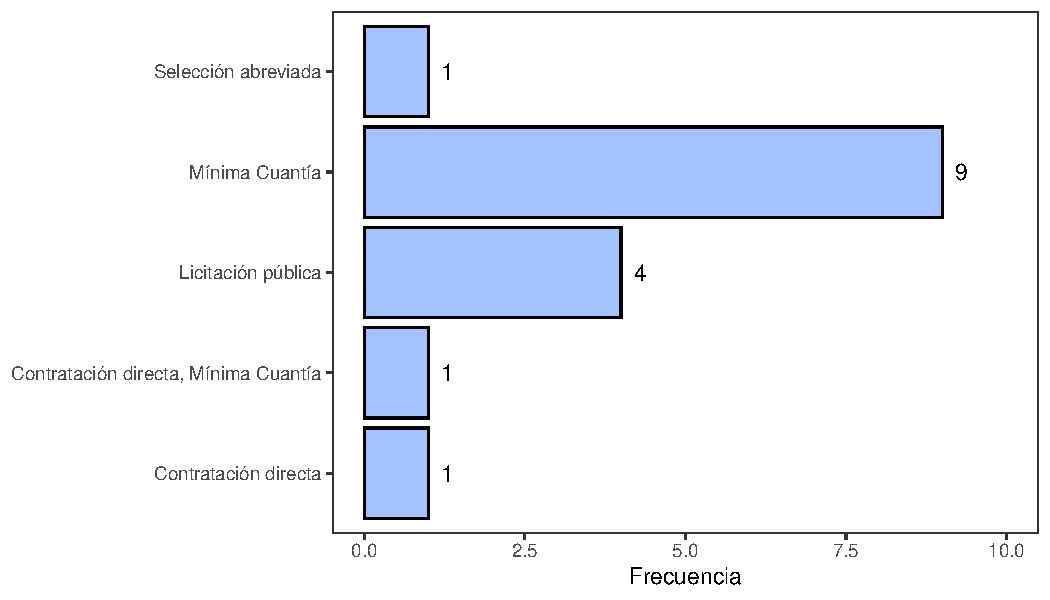
\includegraphics[width=0.85\linewidth]{InformeFinal_files/figure-latex/modalidadAdquisicion-1} 

}

\caption{Modalidad de selección para contratos de adquisición de recetarios}\label{fig:modalidadAdquisicion}
\end{figure}

De acuerdo con los entes territoriales, esta modalidad de selección presenta favorabilidad desde el punto de vista financiero respecto a la inversión y recaudo posterior tras la venta de los recetarios oficiales. El ingreso por venta de recetarios es una de las principales fuentes de financiación de varios FRE (ver Figura \ref{fig:IngresosFRE1}).

La selección por mínima cuantía tiene como desventaja que algunos requerimientos funcionales del objeto a contratar pueden ser pasados por alto, y esto puede poner en riesgo el cumplimiento de las especificaciones del usuario en cuanto a los recetarios recibidos. De hecho, se observaron ejemplos donde debido a la falta de: (i) verificación de la experiencia del proponente, (ii) seguimiento y/o (iii) auditoria del avance de entrega, se recibieron recetarios no conformes, con prescripciones sin codificación o tintas desgastadas.

La segunda modalidad de selección más frecuente fue licitación pública, en la cual se exige demostrar tiempo de experiencia relacionada a la elaboración de este tipo de insumos. Por ejemplo, sí el recetario cuenta con medidas de seguridad específica (ver Figura \ref{fig:MedidasSeguridad-Almacenamiento}) se espera que el proponente logre demostrar la capacidad de cumplir con la entrega del producto especificado.

Los departamentos con mayor número de características de seguridad en el recetario oficial suelen realizar la contratación mediante licitación pública. Esta modalidad de selección podría favorecer la calidad del producto recibido y esto podría evitar problemas por falsificación del recetario. Sin embargo, en varios departamentos se podrían tener problemas para implementar esta modalidad debido a la falta de oferentes.

Entre las medidas de seguridad más observadas en los recetarios por licitación pública se encuentran el uso de tintas invisibles o fluorescentes en secciones específicas del recetario que brillan bajo la luz UV, bandas y/o filamentos de seguridad, versus las medidas de seguridad de recetarios realizados por mínima cuantía como seriales con codificaciones alfanuméricas, escudo de la gobernación respectiva y/o marcas de agua.

Pese a que la modalidad de selección en los contratos de adquisición de recetarios es un factor que afecta de forma importante el costo, se debe tener en cuenta que en algunos departamentos existe un rubro dentro de la gobernación para papelería y de este mismo se compran los recetarios, sin tener conocimiento del valor destinado para estos insumos por parte del FRE.

En el marco de las actividades de las Jornadas de inmersión territorial, se logró observar un patrón en el proceso de licitación y contratación de recetarios oficiales por los FRE alrededor del país. Como se evidencia en la Figura \ref{fig:procesoContractual}, en la mayoría de los casos, los funcionarios de los FRE se encargan exclusivamente de la realización de los estudios previos, en donde se solicita la necesidad en cantidad y forma de recetarios. Posterior a ello, es la dirección territorial en salud, que en algunos casos es la secretaria de salud departamental, la gobernación u otra dependencia con interés en la salud pública del territorio, la encargada de desarrollar la etapa contractual del proceso, mediante una de las modalidades de selección de oferentes que más convenga, se elige la empresa proveedora y se establece el contrato de elaboración de recetarios oficiales.

\begin{figure}

{\centering 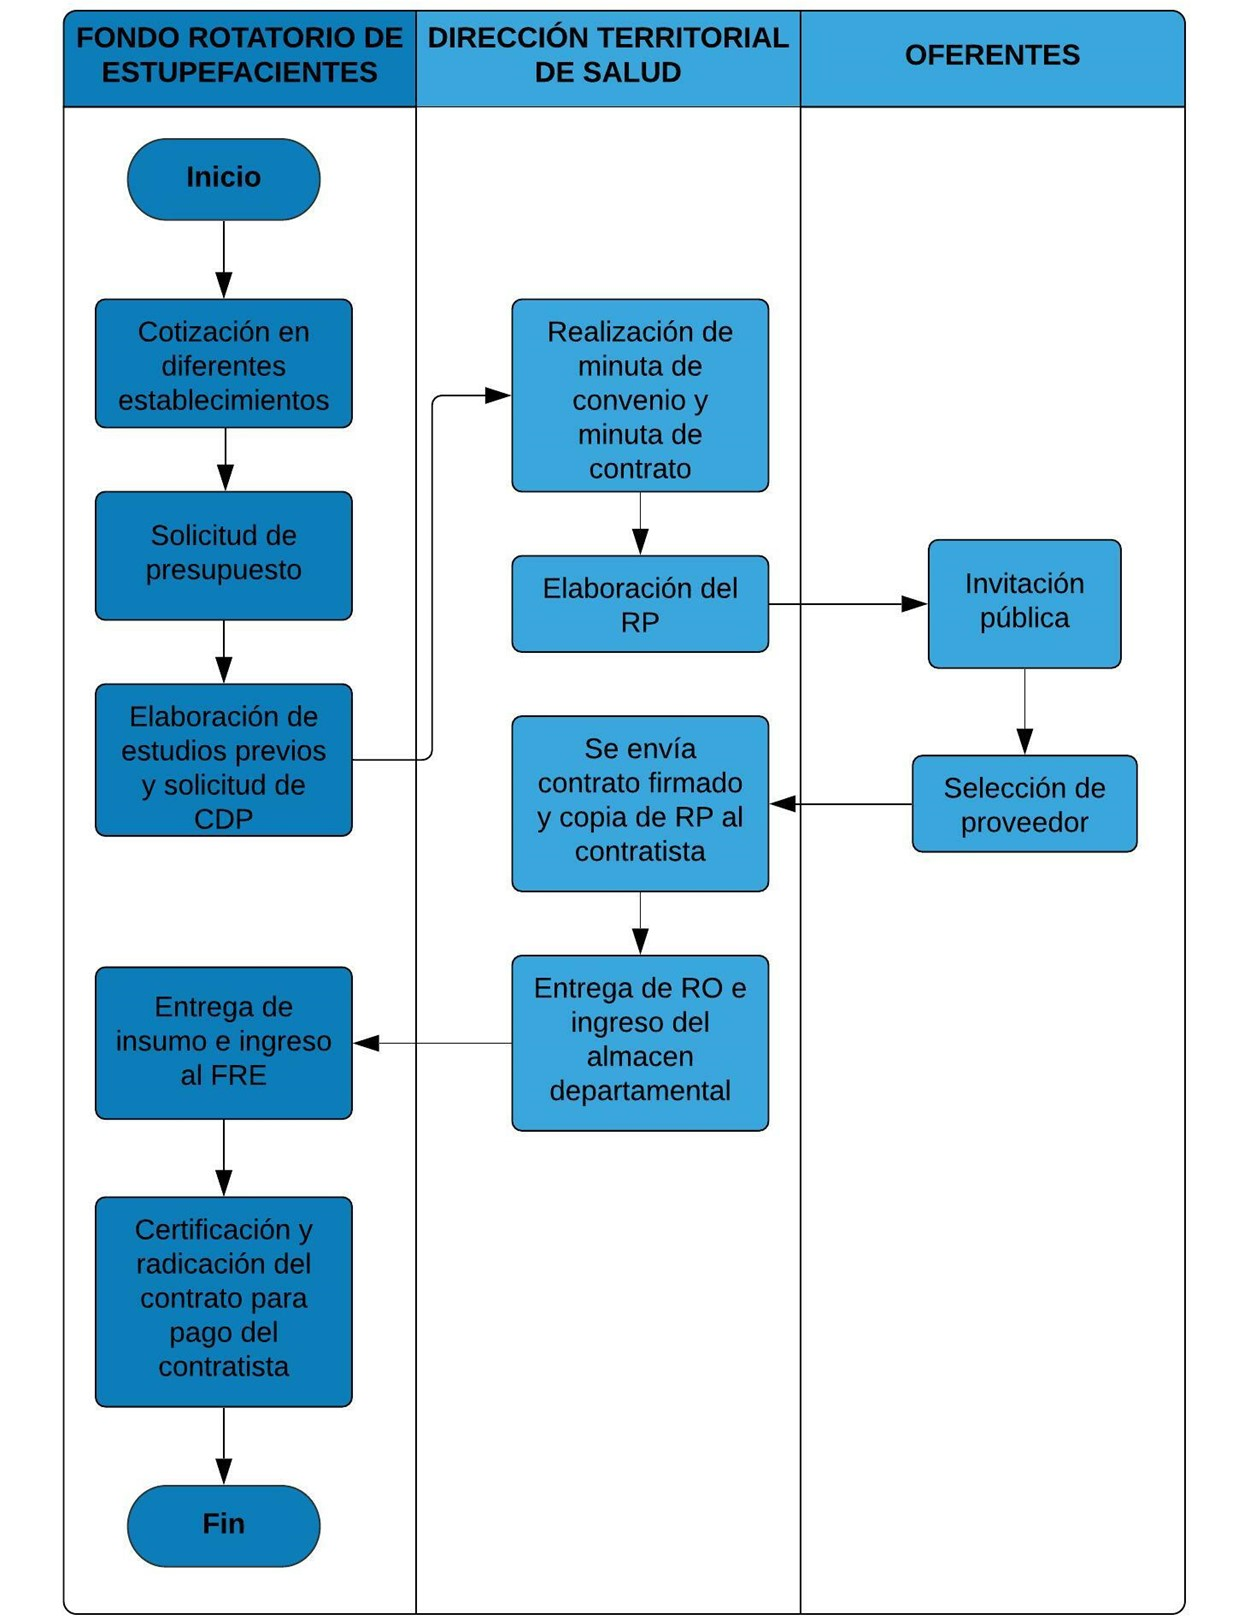
\includegraphics[width=0.8\linewidth]{figures/procesoContractual} 

}

\caption{Proceso de contratación/licitación de los recetarios oficiales.}\label{fig:procesoContractual}
\end{figure}

\hypertarget{tiempos-de-adquisiciuxf3n}{%
\subsection{Tiempos de adquisición}\label{tiempos-de-adquisiciuxf3n}}

\begin{figure}

{\centering 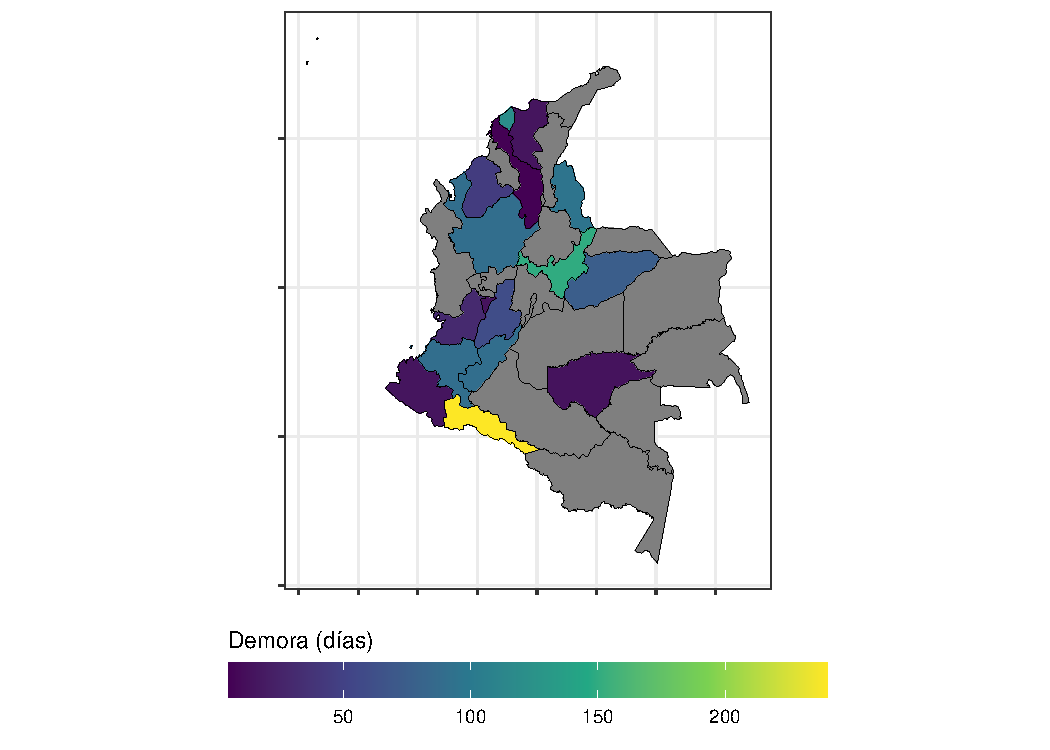
\includegraphics[width=0.85\linewidth]{InformeFinal_files/figure-latex/tiempoDemoraAdquisicion-1} 

}

\caption{Tiempo de demora para adquisición de recetarios}\label{fig:tiempoDemoraAdquisicion}
\end{figure}

En la Figura \ref{fig:tiempoDemoraAdquisicion} se muestra el tiempo promedio que toma el proceso de adquisición de recetarios oficiales por parte de los entes territoriales, se evidencia que el tiempo promedio se encuentra entre 60 y 120 días (2 a 4 meses).

Por otro lado, se observó que los departamentos que compran los recetarios por la modalidad de contratación directa son aquellos con menores tiempos de adquisición, tiempos de aproximadamente 1 mes. Mientras que, los departamentos que compran por medio de mínima cuantía y licitación pública tienen mayor variabilidad en el tiempo de adquisición que pueden tardar entre 1 a 8 meses.

La \emph{etapa precontractual} (estudios previos, estudios de mercado y estimación de necesidad) del proceso de adquisición suele ser realizada por el personal del FRE. Estos procesos iniciales toman poco tiempo y suelen tomar entre 1 semana y 2 meses.

Por otra parte, la \emph{etapa contractual} suele ser realizada por la gobernación y puede tardar en completarse de 1 a 2 meses, o en casos particulares más de 2 meses. Estos tiempos estimados en la etapa contractual fueron informados por los FRE, sin embargo, los mismos desconocen el detalle el proceso que se lleva a cabo.

La etapa de despacho de los recetarios puede tomar entre 1 a 3 meses en ejecutarse por parte de los contratistas, y estos tiempos son particulares para cada departamento dependiendo del volumen de recetarios adquiridos y el nivel de especificación acordado, entre otros.

Existen casos atípicos como el FRE del departamento de Putumayo, el cual lleva sin concretar la compra de recetarios oficiales desde el mes de noviembre del año 2020. La principal problemática de adquisición del FRE Putumayo es debida a dificultades de la gobernación con el proceso de licitación.

En algunos departamentos se utiliza la plataforma Colombia Compra Eficiente para la adquisición de recetarios. Se encuentran algunos departamentos que han experimentado dificultades con esta plataforma y esto ha resultado en demoras en el proceso de adquisición de recetarios.

\hypertarget{procesos-relacionados-a-los-recetarios}{%
\section{Procesos relacionados a los recetarios}\label{procesos-relacionados-a-los-recetarios}}

\maxdeadcycles=1000

\hypertarget{recepciuxf3n-de-recetarios}{%
\subsection{Recepción de recetarios}\label{recepciuxf3n-de-recetarios}}

En relación con la Figura \ref{fig:ReciboRecetariosInstituciones}A, se puede observar que 17 de los FRE entrevistados confirmaron que, sí reciben los recetarios diligenciados de las instituciones inscritas en su despacho dentro de los tiempos estimados, ver Figura \ref{fig:ReciboRecetariosInstituciones}B. Esto se realiza con el fin de corroborar los informes allegados correspondientes al anexo 13 que se entregan mensualmente.

\begin{figure}

{\centering 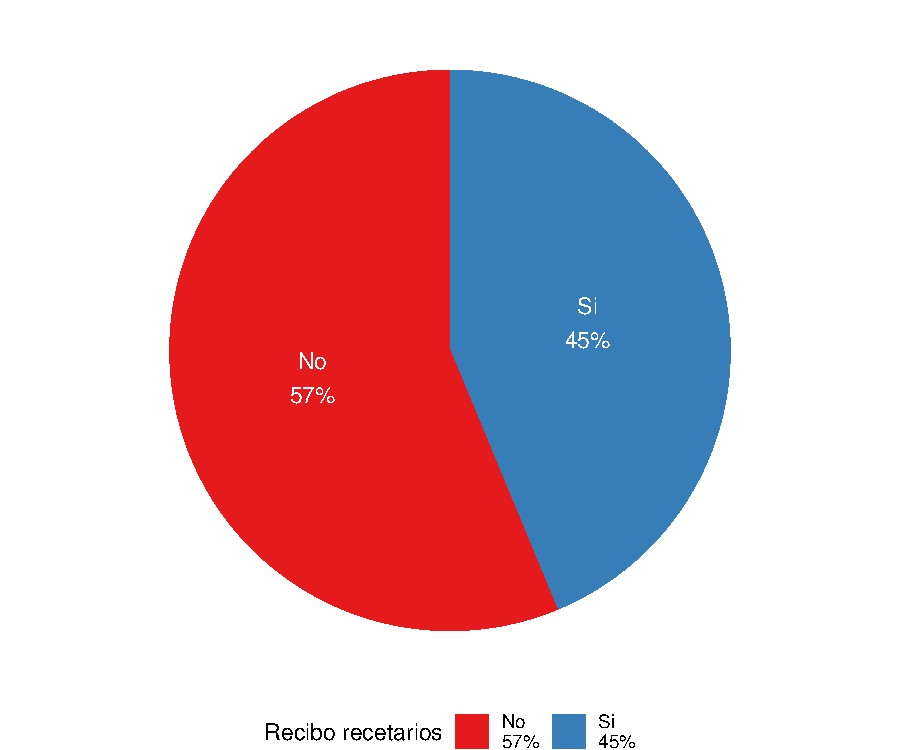
\includegraphics[width=1\linewidth]{InformeFinal_files/figure-latex/ReciboRecetariosInstituciones-1} 

}

\caption{Recepción de recetarios. Panel A. Porcentaje de entes territoriales que reciben recetarios oficiales recibidos prescritos/diligenciados. Panel B. Tiempo de recepción de recetarios oficiales desde IPS.}\label{fig:ReciboRecetariosInstituciones}
\end{figure}

Los recetarios entregados deben revisarse exhaustivamente para evidenciar el buen uso de estos. Junto con los recetarios se trae el anexo 13 para corroborar que los medicamentos formulados coincidan con los valores prescritos en cada uno de los mismos. Esta tarea se realiza en 17 de los 31 departamentos visitados, sin embargo, es una actividad demorada debido a la: (a) falta de personal en los entes territoriales y (b) cantidad de instituciones inscritas y/o médicos prescriptores que hay en el departamento.

El resto de los departamentos (57\%) no reciben los recetarios prescritos en físico, entre las razones, la más frecuente está relacionada con la capacidad de almacenamiento del FRE de este tipo de documentación, que suele ser muy limitado o no se cuenta con el mismo. En dichos casos, los FRE han optado por emitir circulares, solicitando a las entidades y médicos prescriptores inscritos que mantengan la custodia de los talonarios diligenciados, como parte de la historia clínica de los pacientes, hasta que el FRE realice la visita de inspección, vigilancia y control. Una vez allí, se realiza un muestreo para verificar que las fórmulas prescritas en un determinado tiempo concuerden con las cantidades de medicamentos reportados en los informes mensuales.

\hypertarget{venta-de-recetarios-oficiales}{%
\subsection{Venta de recetarios oficiales}\label{venta-de-recetarios-oficiales}}

El proceso de venta de recetarios oficiales se lleva a cabo de forma estandarizada en el grueso de los FRE del país, siguiendo el procedimiento descrito en la Figura \ref{fig:procesoVentaRec}. Allí se observa se forma generalizada la primera instancia del proceso, la cual es la solicitud de cotización de recetarios oficiales al FRE. Esta puede ser de forma personal o vía correo electrónico. Posterior a ello, el ente territorial realiza su estudio interno de disponibilidad y responde a la institución interesada con la cantidad que puede vender, de ser el caso en que no disponga del total de recetarios que el establecimiento farmacéutico requirió.

\begin{figure}

{\centering 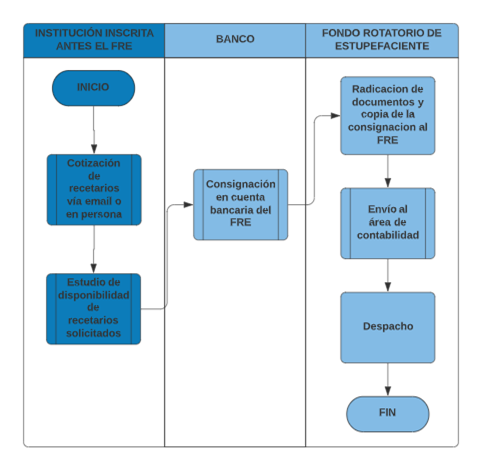
\includegraphics[width=0.8\linewidth]{figures/procesoVentaREC} 

}

\caption{Proceso de venta de recetarios oficiales}\label{fig:procesoVentaRec}
\end{figure}

Según la Resolución 1479 de 2006\textsuperscript{\protect\hyperlink{ref-MSPS1479-2006}{1}} - articulo 3, cada FRE debe contar con una cuenta bancaria en donde administre sus operaciones. En esta cuenta es donde la institución interesada deposita el monto de la cotización realizada. Finalmente, se radica ante el FRE el soporte de pago y los documentos de la cotización para que sean enviados al área de contabilidad del ente territorial, y los recetarios despachados al establecimiento farmacéutico que los requiere.

Este proceso de venta de recetarios oficiales se desarrolla de forma rápida como lo demuestra la Figura \ref{fig:TiempoVentaInstituciones}. En la mayoría de departamentos tarda entre 1 y 2 días concretar la venta, tiempo que es determinado realmente por el establecimiento y cuanto demore en hacer el pago bancario a la cuenta del FRE. Los casos particulares en que el proceso toma hasta 5 días o más, como es el caso particular del FRE de Norte de Santander, se da por el alto riesgo de desvíos y posibilidad de fraudes de recetarios oficiales, por lo que los funcionarios del ente territorial, se toman una semana para realizar exhaustivamente la revisión del comprador. Por otro lado, en los FRE de Huila, Tolima y Vaupés, este comportamiento se presenta principalmente por falta de personal que pueda abarcar el total de las actividades que debe desarrollar el ente territorial, panorama común dentro de lo observado a lo largo de los acompañamientos técnicos del Proyecto de inversión Misión PRI 1901 a los distintos FRE de la nación, en donde por carencia de personal suficiente se tienen que priorizar unas tareas y relegar otras actividades del ente territorial igualmente valiosas para la salud pública de la región.

\begin{figure}

{\centering 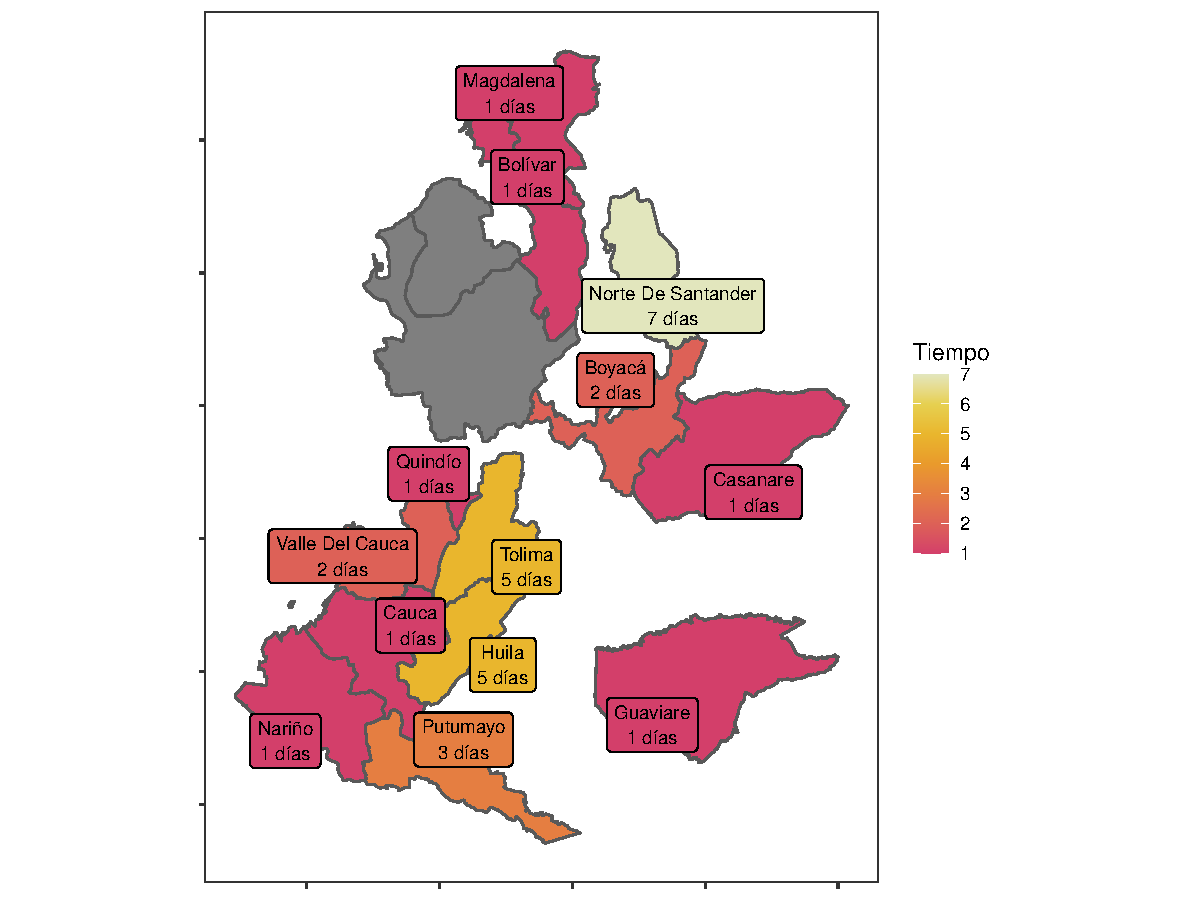
\includegraphics[width=0.9\linewidth]{InformeFinal_files/figure-latex/TiempoVentaInstituciones-1} 

}

\caption{Tiempo de demora en la venta de recetarios oficiales a clientes}\label{fig:TiempoVentaInstituciones}
\end{figure}

\hypertarget{seguimiento-a-uso-de-recetarios}{%
\subsection{Seguimiento a uso de recetarios}\label{seguimiento-a-uso-de-recetarios}}

La Figura \ref{fig:BD-diligBDRecet} muestra los campos de información recolectada en bases de datos por los FRE al momento de realizar la venta de un recetario oficial, la información recolectada permite conocer entre otras cosas:

\begin{itemize}
\item
  Datos básicos de las entidades y prescriptores inscritos en el FRE.
\item
  Unidades consumidas y su respectivo valor.
\item
  Datos de identificación de los recetarios.
\item
  Número de talonarios que se distribuyen en los respectivos departamentos.
\end{itemize}

\begin{figure}

{\centering 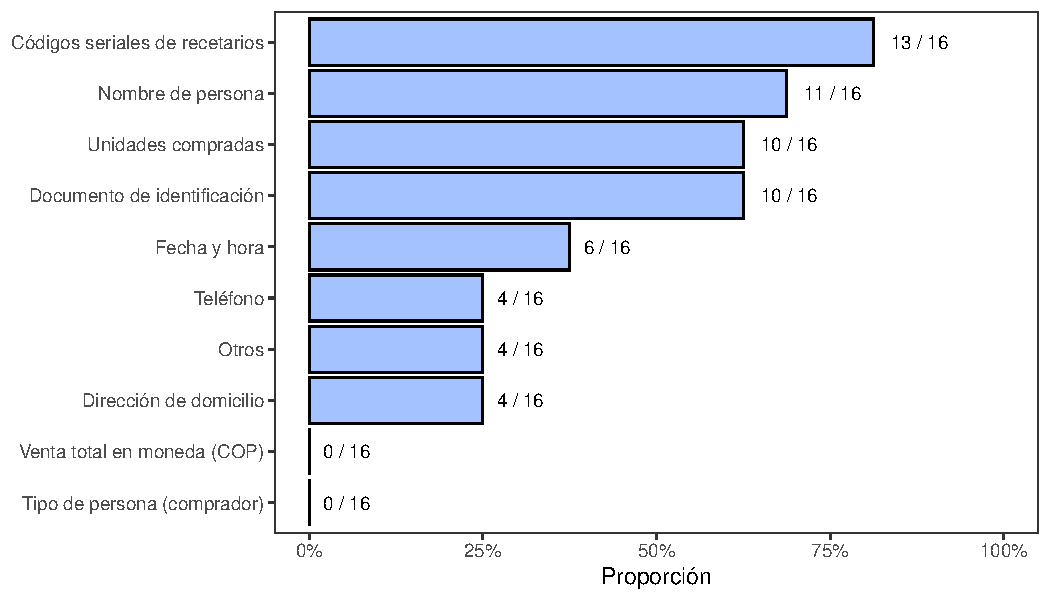
\includegraphics[width=0.85\linewidth]{InformeFinal_files/figure-latex/BD-diligBDRecet-1} 

}

\caption{Proporción de FRE que diligencian campos en BD de venta de recetarios}\label{fig:BD-diligBDRecet}
\end{figure}

Durante la jornada de inmersión territorial, se puedo observar que los FRE utilizan dichas bases con dos propósitos principales:

\begin{itemize}
\item
  Realizar estimaciones de necesidad de recetarios, control de inventarios y control en las cantidades que los compradores adquieren. Esto permite llevar un seguimiento del consumo promedio de las entidades. Este control permitió a los FRE realizar un seguimiento a posibles desvíos o anormalidades en los consumos. Por ejemplo, con el inicio de la pandemia el consumo de ROs y MME aumentó en la mayoría de los departamentos, por lo que los FRE tuvieron que fortalecer el trabajo en equipo con las entidades para mitigar desabastecimientos.
\item
  Evitar fraudes o falsificaciones al realizar un control en el manejo de talonarios, y contrastando la información de las bases con la entregada o solicitada durante visitas.
\end{itemize}

Se observó que la mayoría de FRE (proporción mayor a 50\% en la Figura \ref{fig:BD-diligBDRecet}) llevaban un control de información con el fin de identificar a los compradores (Nombre del comprador persona o institución) y las cantidades adquiridas -- Unidades compradas. Se almacenan datos de contacto, como dirección o teléfono en tan solo 25\% de los FRE. Por otro lado, se evidenció que la mayoría de departamentos (83\%) optan por realizar seguimiento a los recetarios con el código de serial, debido a que estos son únicos en cada recetario.

Así mismo, se observaron otros tipos de campos almacenados por los FRE (opción Otros) en la venta de recetarios. Entre estos otros se encuentra: (a) consecutivos de las facturas emitidas en cada compra, (b) registro REPS, (c) saldo de recetarios oficiales tras la compra, o (d) códigos de recetarios oficiales prescritos allegados para su revisión. Algunos FRE cierran el ciclo de control del RO, en la misma base de datos, al relacionar los RO prescritos que son devueltos para su revisión.

Los FRE realizan una serie de actividades para el seguimiento de uso de los recetarios. En la Figura \ref{fig:SeguimientoUsoRecetarios} se muestra las distintas acciones realizadas por parte de los FRE para el seguimiento al manejo de los RO. La actividad de control más realizada, alrededor de un 70\%, es la visita a las instituciones y médicos independientes inscritos en el FRE. La dinámica principal de la visita consiste en actividades propias de IVC, y a su vez en la revisión del anexo 13 junto con otros informes particulares vs las copias de las prescripciones de los RO que las entidades tengan disponibles.

Las visitas a instituciones han permitido evidenciar en algunos departamentos, falencias en el uso adecuado de los RO, como por ejemplo prescripciones en las cuales se formulan antibióticos u otros medicamentos en conjunto con MME o solos, así mismo se tienen casos donde se encuentran recetarios en blanco, pero con firma y sello del médico prescriptor, generando un alto riesgo de desvío en las instituciones.

En segundo lugar, se encuentra la verificación de base de ventas. Esta actividad se explicó al mencionar que las mismas se utilizan para el control y seguimiento de posibles desvíos o anormalidades en los consumos.

Las actividades anteriormente descritas se consideran actividades de seguimiento pasivas, caso contrario a la verificación de recambios. Esta actividad se realiza en un 22\% del territorio Nacional, la cual consiste en autorizar la venta de recetarios a las entidades y/o médicos prescriptores solo sí devuelve los recetarios comprados anteriormente. Por parte de los departamentos se aclara que no es necesarios vender la misma cantidad de recetarios que el comprador devuelve.

Otras actividades de seguimiento activo al manejo de RO son el seguimiento a las denuncias, las cuales tienen una proporción menor al 5\%. Finalmente, el acompañamiento permitió evidenciar que el 15\% de los FRE no realizan ningún tipo de actividad de seguimiento al uso de los ROs, tan solo cumpliendo con la presentación de informes exigidos por la normativa vigente.

\begin{figure}

{\centering 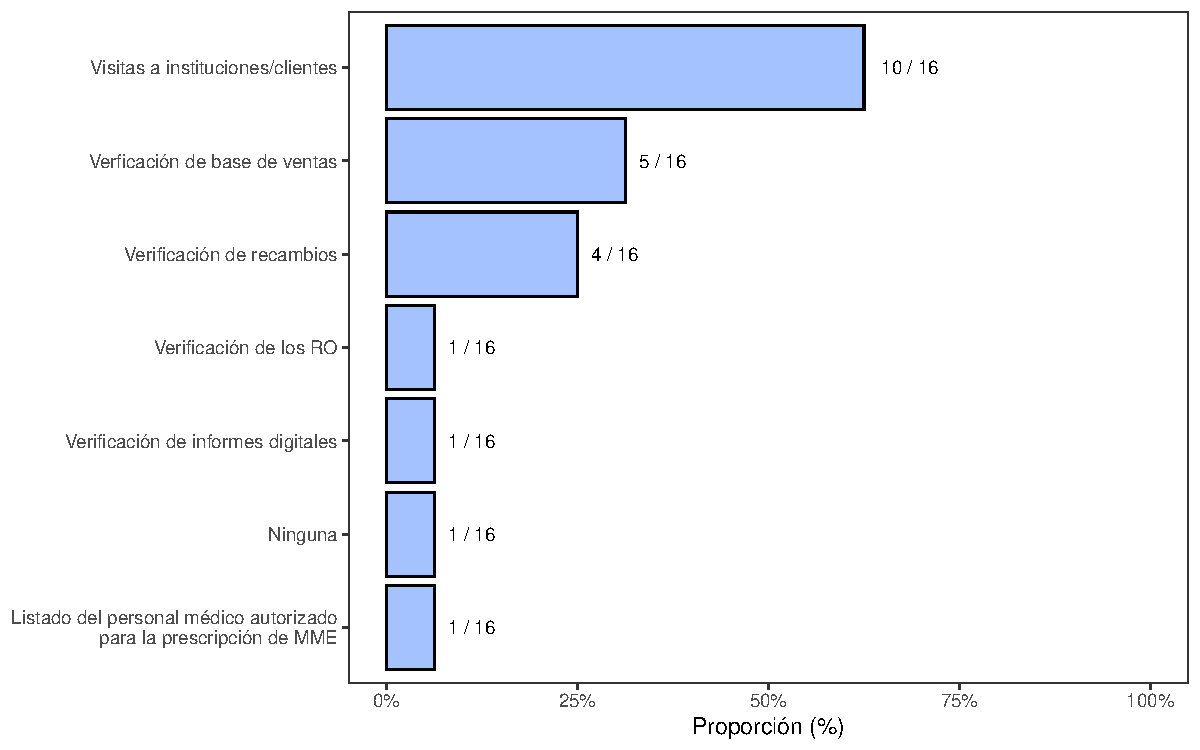
\includegraphics[width=0.85\linewidth]{InformeFinal_files/figure-latex/SeguimientoUsoRecetarios-1} 

}

\caption{Actividades realizadas por el FRE para el seguimiento del uso de recetarios}\label{fig:SeguimientoUsoRecetarios}
\end{figure}

\hypertarget{archivo-de-recetarios}{%
\subsection{Archivo de recetarios}\label{archivo-de-recetarios}}

Durante el acompañamiento se complementó como recomendación a los FRE, se considerará alinearse a lo expresado en la Circular 009 de 2015 del FNE, donde se difunde la buena práctica de implementar bases de retención documental y gestión de archivo\textsuperscript{\protect\hyperlink{ref-FNE2015-9}{8}}. La frecuencia con la cual se reciben los recetarios oficiales a los FRE desde las entidades y médicos prescriptores inscritos se observa en la Figura \ref{fig:ReciboRecetariosInstituciones}B La frecuencia de recepción de recetarios guarda relación con la información analizada en el punto anterior. Se tiene que 13 FRE reciben los 10 primeros días del mes los recetarios oficiales prescritos conforme a lo solicitado a las instituciones de cada departamento, mientras que los otros 4 FRE no han estandarizado el tiempo de entrega y reciben los recetarios oficiales a lo largo del mes, asegurando su recepción mediante recordatorio por correo electrónico o comunicación telefónica, si llega a ser requerido. Se tiene que 17 de 31 FRE reciben los recetarios oficiales desde IPS.

Complementando la información reportada en la Figura \ref{fig:ReciboRecetariosInstituciones} y en la Figura \ref{fig:TiempoArchivoRecetariosOficiales}, se relacionó el tiempo de archivo que los FRE que si reciben los recetarios oficiales los almacenan, obteniendo que 10 FRE los almacenan por un periodo mayor a 5 años. Durante las jornadas de inmersión territorial se pudo observar que este tiempo de almacenamiento, en la mayoría de los casos, es por desinformación en los FRE, puesto que no se tiene presente el tiempo que se deben guardar estas copias, y al considerarlas parte de la historia clínica de un paciente estiman guardarlas hasta por 10 años, superando en muchos casos la capacidad de archivo de los FRE.

\begin{figure}

{\centering 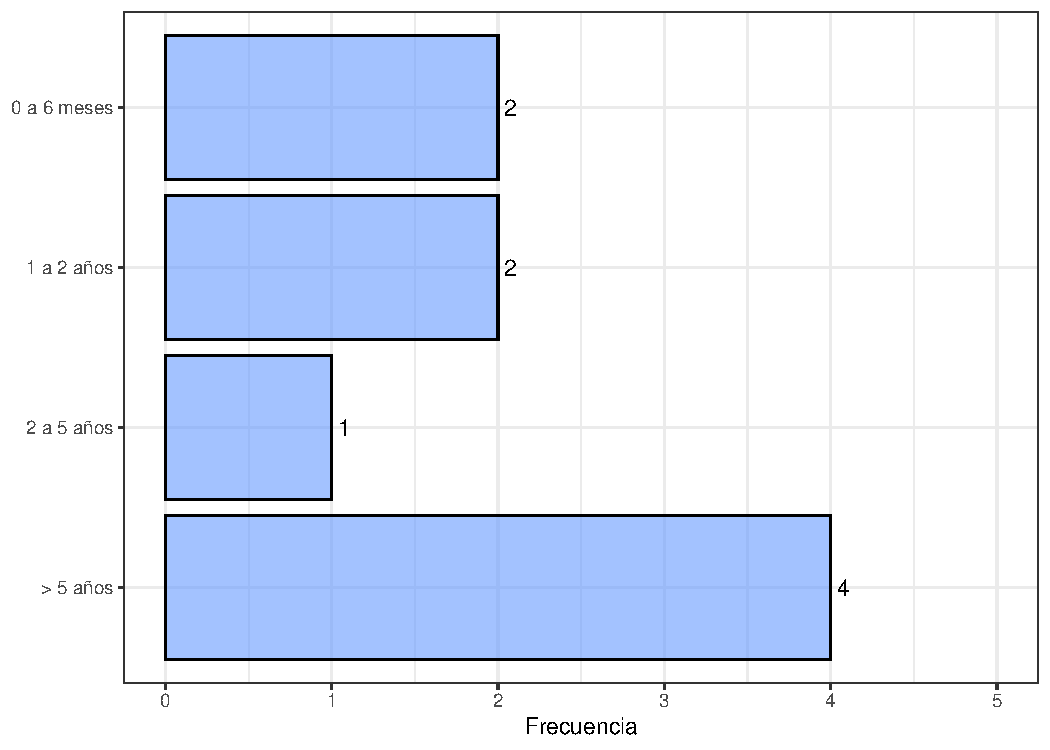
\includegraphics[width=0.85\linewidth]{InformeFinal_files/figure-latex/TiempoArchivoRecetariosOficiales-1} 

}

\caption{Tiempo de archivo de los recetarios oficiales en los FRE}\label{fig:TiempoArchivoRecetariosOficiales}
\end{figure}

En otros casos, la intención de archivo se acoge a las medidas establecidas por las gobernaciones, en las cuales se pide un archivo de 20 años para documentación critica, según las tablas de retención documental gubernamental\textsuperscript{\protect\hyperlink{ref-PresidenciadelaRepublicadeColombia2012}{9}}. Otros FRE en cambio establecieron protocolo de archivo y una vez cumplido el periodo de almacenamiento, por supuesto, posterior revisión, los recetarios oficiales son destruidos.

Como se mencionó previamente durante el acompañamiento se compartió la Circular 009 de 2015\textsuperscript{\protect\hyperlink{ref-FNE2015-9}{8}}, la cual en su Artículo Primero expresa:

\begin{quote}
\emph{``Que las autoridades administrativas, los fabricantes, los comerciantes, los hombres de ciencia, las Instituciones científicas y los hospitales lleven registros en que consten las cantidades de cada estupefaciente fabricado, y de cada adquisición y destino dado a los estupefacientes. Dichos registros serán conservados por un periodo de dos años por lo menos. Cuando se utilicen talonarios (artículo 30, inciso 2 b) de recetas oficiales, dichos talonarios se conservarán también durante un periodo de dos años por lo menos''.}
\end{quote}

En este sentido, los FRE buscarán adoptar dicha medida para liberar espacio de almacenamiento, con el fin de que pueda ser aprovechado para otro tipo de insumos.

Debido a que los recetarios oficiales son el requisito obligatorio para la dispensación de medicamentos de control especial o monopolio del estado, se ha visto la necesidad de resguardar los talonarios en áreas seguras y de acceso limitado para evitar robos o desvíos. En la Figura \ref{fig:MedidasSeguridad-Almacenamiento} se observa que todos los departamentos han implementado algún tipo de medida de seguridad para el control de los recetarios.

\begin{figure}

{\centering 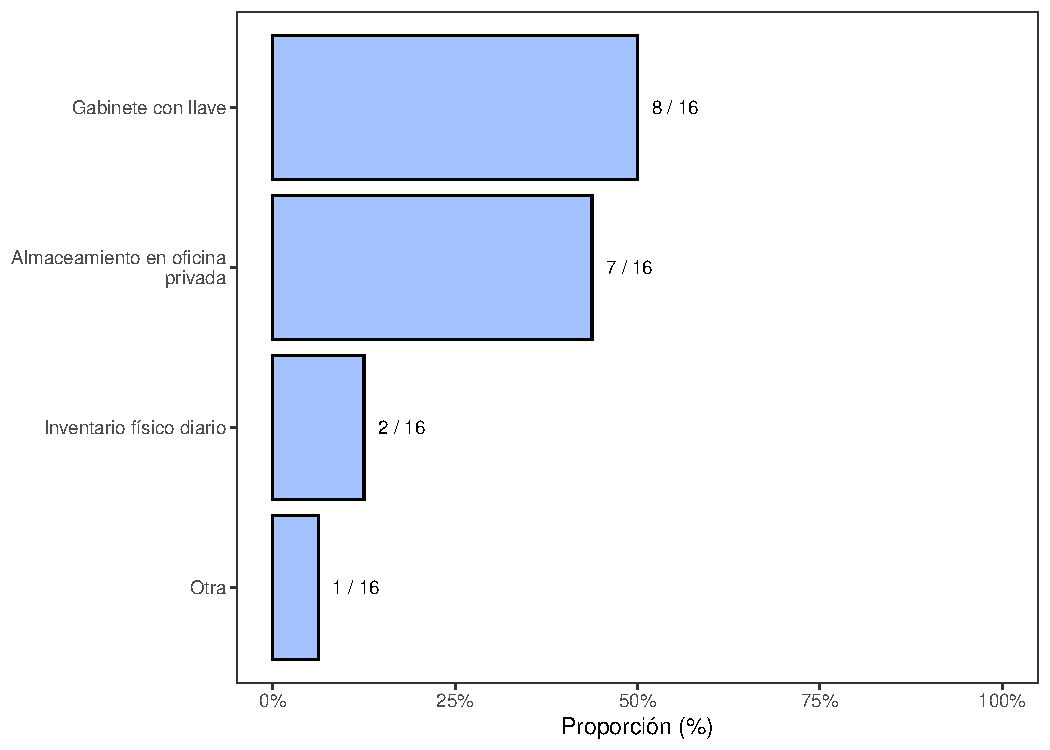
\includegraphics[width=0.85\linewidth]{InformeFinal_files/figure-latex/MedidasSeguridad-Almacenamiento-1} 

}

\caption{Proporción de FRE con medidas de seguridad implementada en almacenamiento de recetarios}\label{fig:MedidasSeguridad-Almacenamiento}
\end{figure}

La mayoría de los FRE, más del 70\%, han optado por almacenar los recetarios oficiales en gabinetes u oficinas privadas con acceso limitado al personal del FRE, con el objetivo de garantizar la custodia de los mismos y evitar pérdidas, de preferencia en espacios que además aseguren su buen estado físico. Hasta el momento, estas medidas de seguridad han sido suficientes puesto que durante el acompañamiento no se encontraron casos en los cuales los FRE hayan mencionado históricos de situaciones de robo o pérdida de recetarios. Sin embargo, durante el proyecto de inversión, especialmente durante las visitas a las que se tuvo acceso presencial o imágenes de las oficinas de almacenamiento, se pudo evidenciar que, si bien los recetarios están almacenados en oficinas privadas o gabinetes con llave, las condiciones para tal fin no son las adecuadas, se tienen situaciones donde se comparten espacios con los medicamentos, y dichos espacios no son suficientes, por lo que se deben disponer en lugares estrechos de las oficinas del FRE.

Adicionalmente, los FRE suelen solicitar mejoras en la infraestructura o seguridad de las oficinas, pero la inversión se ve limitada por autorización y/o estudio de recursos económicos para estos proyectos financiada en la mayoría de los casos por las gobernaciones. Debido a lo anterior, se hace necesario una mejoría en la infraestructura para la mayoría de los Fondos Rotatorios y mejorar las prácticas de almacenamiento.

Por último, sólo 3 departamentos realizan un inventario físico diario, asegurando que los recetarios estén completos. Esta actividad suele hacerse revisando las cajas donde son traídos los recetarios, observando que la cantidad de estas no estén alteradas.

\hypertarget{caracteruxedsticas-de-los-recetarios}{%
\section{Características de los recetarios}\label{caracteruxedsticas-de-los-recetarios}}

\maxdeadcycles=1000

\hypertarget{nuxfamero-de-prescripciones-por-recetario}{%
\subsection{Número de prescripciones por recetario}\label{nuxfamero-de-prescripciones-por-recetario}}

Respecto a las características de los recetarios oficiales que se manejan actualmente en el país, se evidencia la tendencia en los FRE del país es de 50 prescripciones por recetario en 22 FRE, tal cual se observó en las jornadas de acompañamiento técnico realizadas. Seguido de 4 FRE en donde se elaboran los recetarios con 25 prescripciones. También se evidenciaron 3 FRE en donde los recetarios se elaboran con 30, 80 y 100 prescripciones, como lo muestra la Figura \ref{fig:existenciaRecetarios4}. Cabe aclarar que según las normas de regulación de MME y recetarios oficiales, como los son las Resolución 1478 de 2006\textsuperscript{\protect\hyperlink{ref-MSPS1478-2006}{4}} y Resolución 1479 de 2006\textsuperscript{\protect\hyperlink{ref-MSPS1479-2006}{1}}, no se tiene establecido un número de prescripciones por recetario, por lo que los FRE de cada departamento tienen disponibilidad de decidir dicha cuestión.

\begin{figure}

{\centering 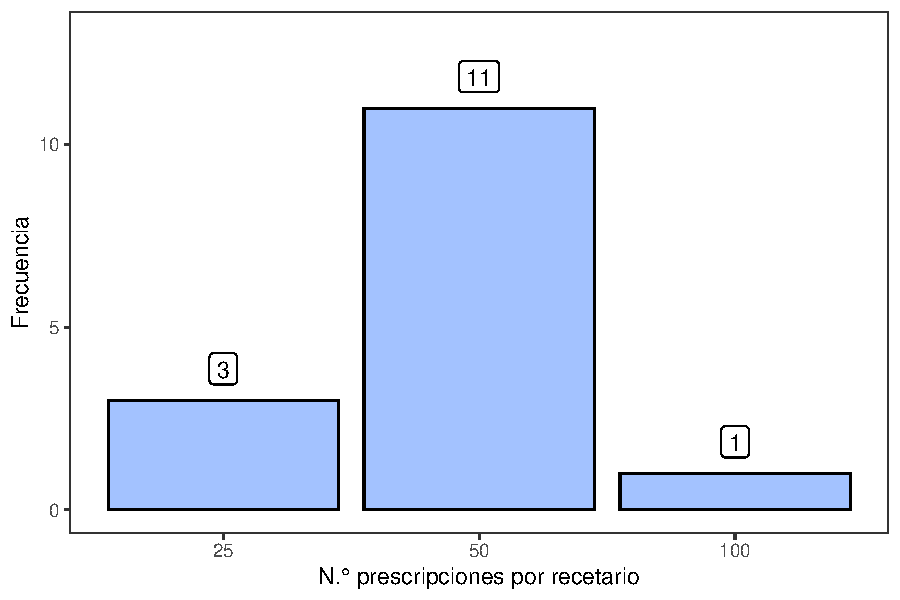
\includegraphics[width=0.85\linewidth]{InformeFinal_files/figure-latex/existenciaRecetarios4-1} 

}

\caption{N.° de prescripciones por recetario}\label{fig:existenciaRecetarios4}
\end{figure}

\hypertarget{medidas-de-seguridad}{%
\subsection{Medidas de seguridad}\label{medidas-de-seguridad}}

Uno de los puntos de acompañamiento del proyecto Misión PRI 1901 era conocer tanto en las visitas presenciales como virtuales, los tipos de medidas de seguridad que se implementan en los recetarios. La Figura \ref{fig:MedidasSeguridadRec} contempló lo mencionado anteriormente, en la cual se observa que existe una gran variedad de medidas consideradas de seguridad en los recetarios, y que existen y existirán tantas como proponentes se tengan. Así mismo, se catalogaron las medidas de seguridad en baja y alta complejidad, teniendo como base lo difícil que pueden llegar a ser falsificados. Se reconoce que todos los departamentos implementaron la codificación en los recetarios oficiales tal y como se menciona en la Resolución 1478 de 2008\textsuperscript{\protect\hyperlink{ref-MSPS1478-2006}{4}} en el Artículo 89 y dicha codificación desarrollada para cada talonario está pensada para ser una identificación única de los mismos.
Tanto como la codificación como las marcas de agua, sellos y escudos se catalogaron como medidas de seguridad de baja complejidad, teniendo en cuenta que hay un riesgo latente de falsificación debido a que las marcas de agua corresponden a figuras particulares o al escudo de la gobernación y/o secretaria de salud, al igual que los sellos y escudos. Sumado a lo anterior, los recetarios están elaborados en papel común y corriente, lo que podría aumentar la probabilidad de ser falsificados.

\begin{figure}

{\centering 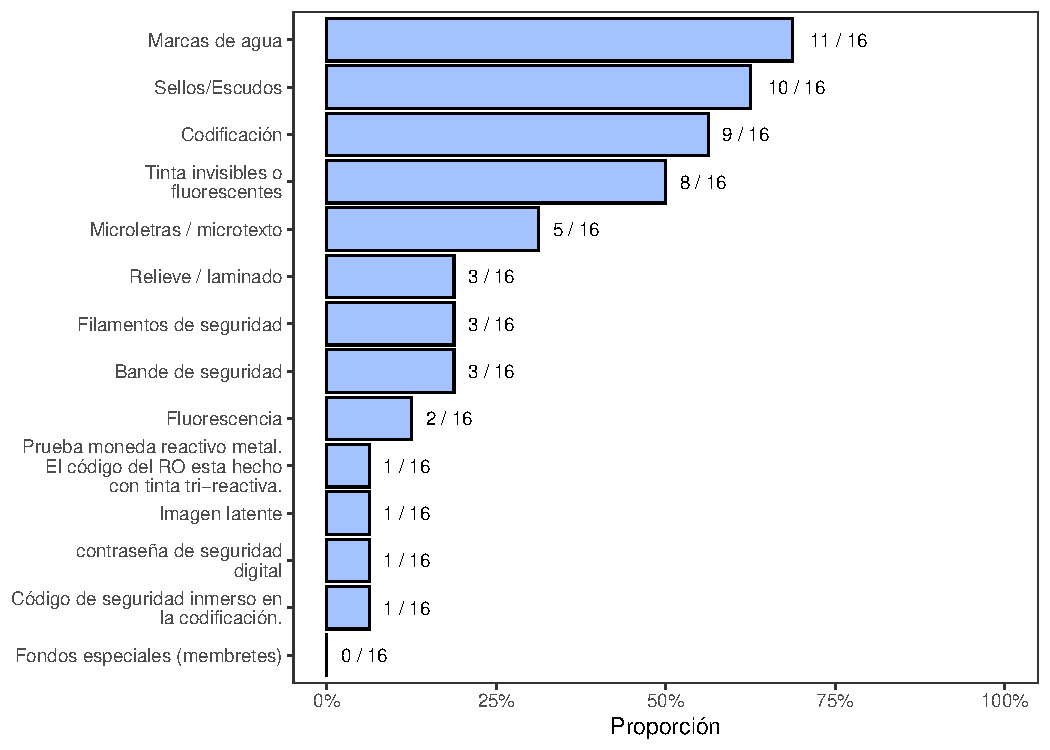
\includegraphics[width=0.9\linewidth]{InformeFinal_files/figure-latex/MedidasSeguridadRec-1} 

}

\caption{Medidas de seguridad en los recetarios}\label{fig:MedidasSeguridadRec}
\end{figure}

Considerando lo anterior, los FRE han optado por implementar niveles de seguridad mayores y elevar la confianza en el manejo de los recetarios, entre estas medidas se observan las siguientes:

\begin{itemize}
\item
  Tintas invisibles o fluorescentes que brillan al estar frente a la luz UV.
\item
  Microletras/microtextos, los cuales están inmersos en cada folio del recetario donde se describe para quien va cada copia.
\item
  Relieves o laminados observados en la copia original de los recetarios.
\item
  Filamentos o bandas de seguridad tecnología similar a los billetes.
\item
  Pruebas reactivo metal, que consisten en raspar un espacio determinado del recetario con un metal o moneda desde la página original del mismo y automáticamente los folios continuos se marcarán.
\item
  Códigos QR que codifican información del año en el cual fue distribuido el talonario.
\end{itemize}

Menos del 40\% de los FRE han implementado medidas de alta seguridad en sus recetarios debido a la capacidad de manufactura de los proveedores departamentales. Dicha limitante se identificó en especial en las regiones alejadas del centro del país, donde en términos de los FRE, los proveedores departamentales no tienen la capacidad o la tecnología suficiente para elaborar un talonario con características de alta seguridad. Además, adquirir contratos con proveedores externos al departamento dificulta el seguimiento o alarga los procesos de compra, por lo que supone superar las barreras geográficas y/o sociales de algunos departamentos.

Al inicio del proyecto de inversión, se estimaba que los recetarios oficiales con más características de seguridad (independiente de su nivel de complejidad) aumentarían de forma proporcional su costo de adquisición y del mismo modo su precio de venta, sin embargo, se evidenció una tendencia totalmente diferente que se puede observar en la Figura \ref{fig:ComparativoCostosRec1} y Figura \ref{fig:DependParcial1}, entre más características de seguridad implementadas en un recetario, éste tiende a ser más económico en su costo de adquisición.

\begin{figure}

{\centering 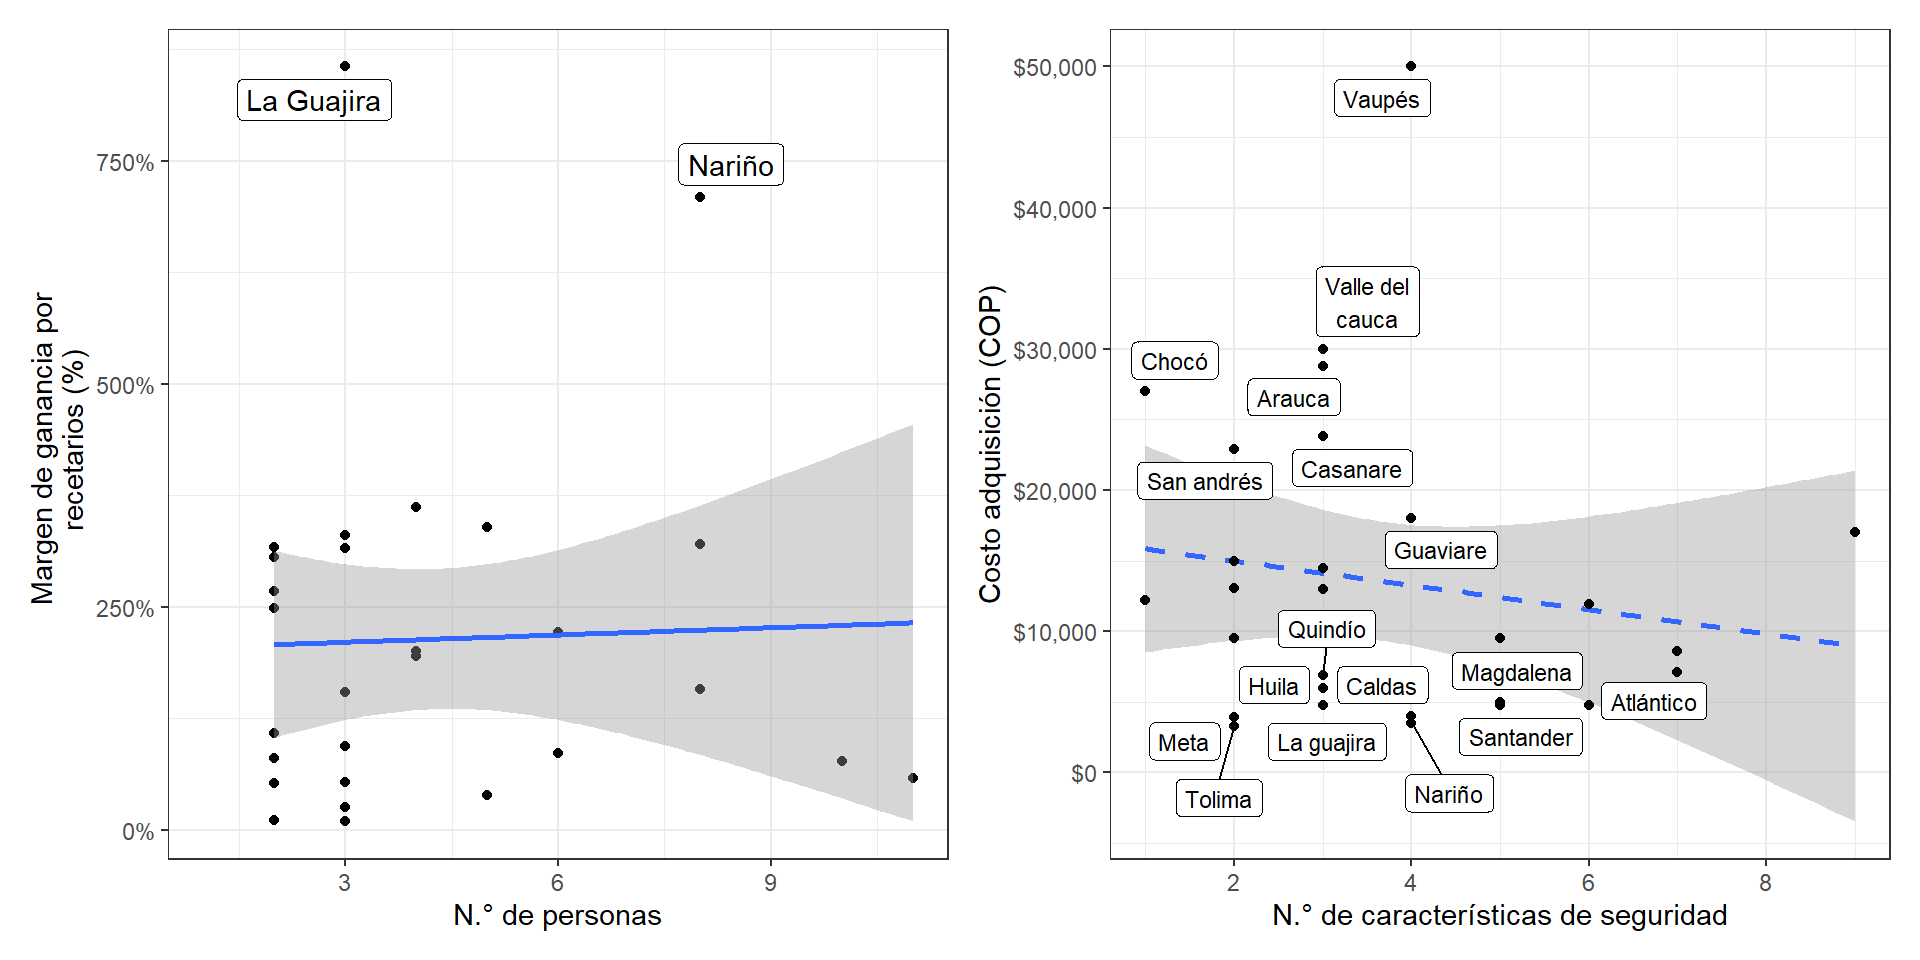
\includegraphics[width=1\linewidth]{InformeFinal_files/figure-latex/ComparativoCostosRec1-1} 

}

\caption{Comparativo de márgen de ganancia de recetarios}\label{fig:ComparativoCostosRec1}
\end{figure}

Por otro lado, se observa el margen de ganancia obtenido mediante la venta de recetarios en los fondos rotatorios, este ítem ya se analizó anteriormente con la Figura \ref{fig:comparativoDepartamentos0}. Sin embargo, no se encuentra una relación entre este margen de ganancia con el número de personas que trabajan dentro del FRE.

Si bien las ganancias obtenidas por las ventas de recetarios son unas de las fuentes principales de ingresos en los entes territoriales, no hay claridad de cómo se manejan estos valores debido a que departamentos con los mismos márgenes de ganancia tienen condiciones distintas, tanto en personal como en infraestructura tecnológica y estructural.

\hypertarget{recetario-oficial-electruxf3nico}{%
\section{Recetario Oficial Electrónico}\label{recetario-oficial-electruxf3nico}}

El recetario oficial es \ldots{}

\hypertarget{opiniones-sobre-el-roe}{%
\subsection{Opiniones sobre el ROE}\label{opiniones-sobre-el-roe}}

\begin{figure}[t]

{\centering 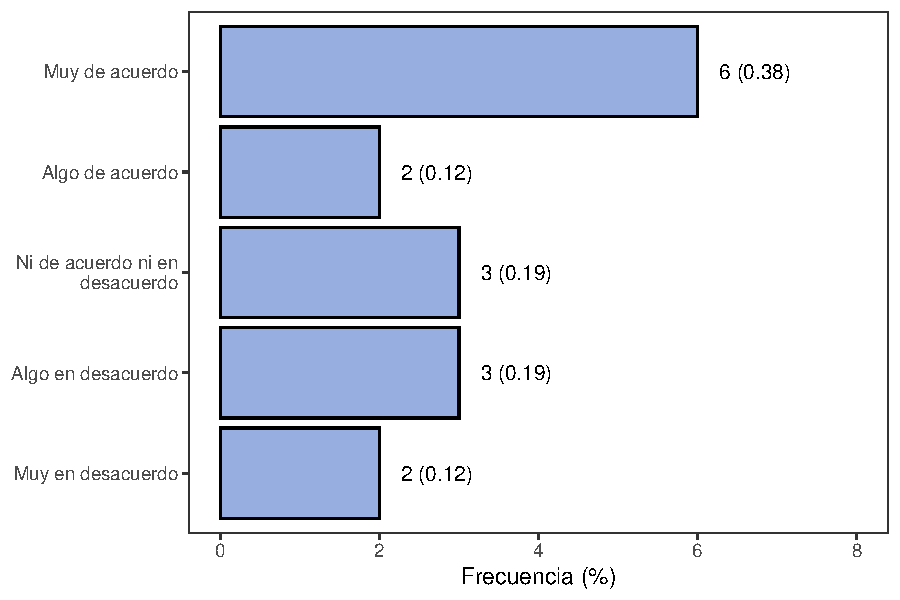
\includegraphics[width=0.85\linewidth]{InformeFinal_files/figure-latex/FREImplementacionROE-1} 

}

\caption{Opinión sobre la implementación del Recetario Oficial Electrónico (ROE)}\label{fig:FREImplementacionROE}
\end{figure}

Como se observa en la Figura \ref{fig:FREImplementacionROE}, el 58\% de los FRE del país tienen una opinión favorable acerca del ROE, ya que, según la información recopilada, los encargados de los diferentes FRE piensan que podría ser una herramienta que brinde mayor seguimiento, trazabilidad y seguridad a las prescripciones de MME, además del ahorro de papel y de espacio de almacenamiento en las bodegas que sería liberado. Como ejemplo de opinión positiva respecto a la implementación del FRE se tiene:

\begin{quote}
\emph{``\ldots{} puede ser un proceso interesante para llevar trazabilidad de los recetarios oficiales. El recetario oficial actual es insuficiente para hacer el respectivo seguimiento y control. Igualmente, el ROE podría mejorar la accesibilidad de medicamentos.''}
\end{quote}

Por otro lado, 29\% de los FRE del país tienen una percepción no favorable acerca de la implementación del ROE principalmente por razones económicas, ya que al dejar a un lado la venta de recetarios oficiales físicos se perdería ese rubro de ingresos al FRE. Adicionalmente, algunos referentes de los entes territoriales manifiestan preocupación por las posibles violaciones de acceso a personal no autorizado, además de los FRE limítrofes, ubicados en regiones con deficiente conexión, afirman que no tendrían la capacidad tecnológica para desarrollar la prescripción por ROE permanentemente a lo que comentan que como medida de contingencia, debería seguir existiendo el recetario oficial en físico, como medida de prevención cuando se pierda acceso a internet en sus territorios, lo que indica la necesidad de realizar campañas de capacitación y educación de uso del ROE antes y durante su implementación como medida prioritaria para el desarrollo de la herramienta digital.

Como ejemplo de opinión negativa se tiene:

\begin{quote}
\emph{``La razón principal es el factor financiero. El FRE necesita los ingresos generados por los recetarios oficiales propios, para su sostenimiento. Igualmente, es difícil continuar con las actividades de seguimiento y control para los recetarios oficiales. Así mismo, podría prestarse para un manejo inadecuado de los MME, contemplando fraude y desvíos en los recetarios oficiales electrónicos.''}
\end{quote}

\hypertarget{lineamientos-para-el-buen-manejo-de-recetarios}{%
\subsection{Lineamientos para el buen manejo de recetarios}\label{lineamientos-para-el-buen-manejo-de-recetarios}}

Tras la recolección de información en el territorio nacional, se encontró que hay fortalezas y debilidades en los departamentos respecto al manejo de los recetarios. Por ende, se hace necesario realizar unos lineamientos técnicos para tener en cuenta y ser adoptados dentro de los entes territoriales, de los cuales se resaltan:

\begin{itemize}
\item
  Tener una espacio exclusivo y seguro para el almacenamiento de los recetarios, en el cual sólo se tenga acceso cierto personal del FRE.
\item
  Realizar un seguimiento de los recetarios por medio de la codificación al momento de venderse, puesto que al no llevar registro de los mismos hay una posibilidad de falsificación y/o desvío.
\item
  Tratar de implementar medidas de seguridad más altas, elevando el nivel de confianza del recetario. En los departamentos donde sólo hay 1 o 2 litografías, se aconseja hablar con dichos proveedores para llegar a un acuerdo de que medidas pueden adicionarse en el recetario. Por ejemplo, adicionar microtextos en cada copia del recetario.
\item
  Seguir las circulares emitidas por el FNE relacionado con el almacenamiento de los recetarios diligenciados, liberándose de espacio en los entes territoriales y teniendo un lugar de trabajo más óptimo.
\item
  Tener niveles de seguridad para realizar la compra de nuevos recetarios, evitando desabastecimientos y llegando a planes de contingencia que pueden llegar a ser reprocesos en los entes territoriales.
\end{itemize}

\hypertarget{manejo-de-medicamentos}{%
\chapter{Manejo de Medicamentos}\label{manejo-de-medicamentos}}

\maxdeadcycles=1000

\hypertarget{adquisiciuxf3n-de-mme-por-parte-del-fre}{%
\section{Adquisición de MME por parte del FRE}\label{adquisiciuxf3n-de-mme-por-parte-del-fre}}

\maxdeadcycles=1000

\hypertarget{control-de-inventarios}{%
\subsection{Control de inventarios}\label{control-de-inventarios}}

El manejo de inventarios es de gran relevancia para las organizaciones que tienen bienes tangibles dispuestos a la venta y cuyo volumen recibido supera el volumen distribuido, como es el caso de los FRE, es por ello por lo que se indago sobre las herramientas que tienen a disposición para el control de inventarios de MME. La mayoría de los FRE realizan el seguimiento de inventarios mediante un paquete ofimático con una proporción de 45.2\% (ver Figura \ref{fig:HerramientasManejoInventarios}), siendo la herramienta principal Excel, con uso especial de hojas estandarizadas, como en el caso de los FRE Boyacá, Cauca, Sucre, entre otros.

\begin{figure}
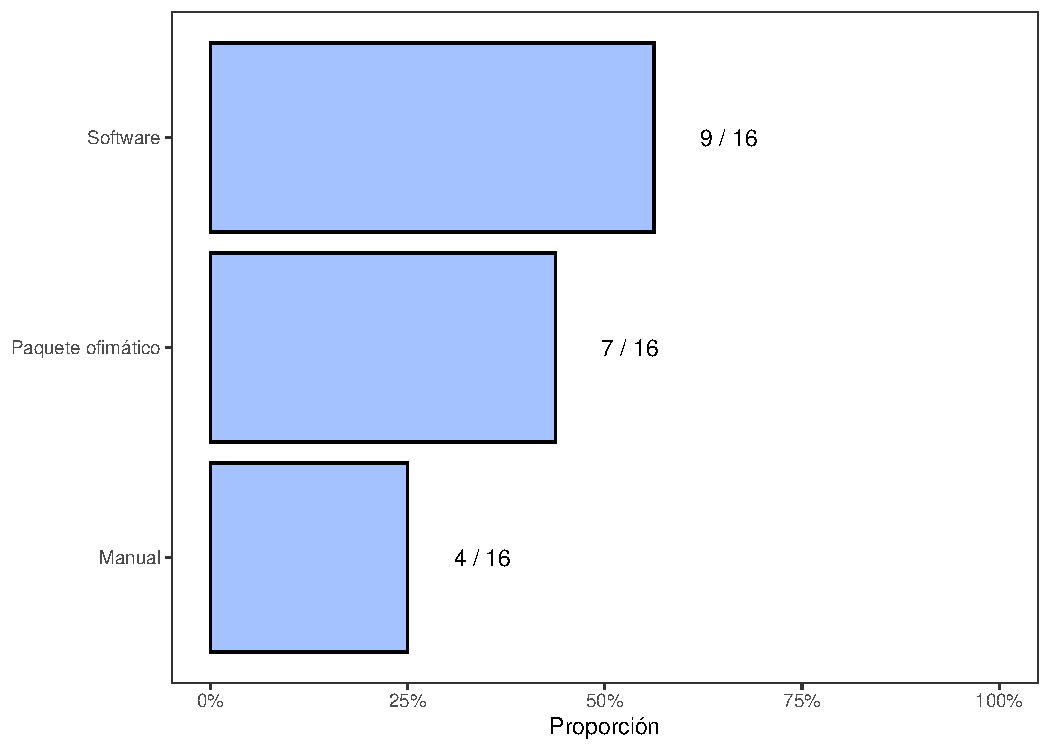
\includegraphics[width=0.85\linewidth]{InformeFinal_files/figure-latex/HerramientasManejoInventarios-1} \caption{Herramientas en el manejo de inventarios}\label{fig:HerramientasManejoInventarios}
\end{figure}

Algunos FRE se apoyan en otras herramientas además del paquete ofimático para llevar a cabo la tarea del control de inventarios. En la segunda posición de la Figura \ref{fig:HerramientasManejoInventarios} se observa el uso de software en una proporción del 38.7\%. La elección del software se hace según los criterios de cada entidad territorial en la mayoría de los casos se utiliza un software interno de la gobernación del territorio para el desarrollo de estas actividades como es el caso de los FRE Atlántico, Cesar, Santander, entre otros.

El alcance del software es distinto, por ejemplo, el caso del FRE Risaralda que hace uso del software SIMEC para soportar tanto el manejo de inventarios, como los procesos relacionados con el sistema de IVC en todo lo relacionado con MME. Este software funciona además como medio de comunicación entre el FRE y todos sus inscritos, mostrándose como una plataforma muy completa y eficiente, sin embargo, existe poca disponibilidad de equipos de cómputo en el FRE que impide que más personal pueda acceder al software y a sus herramientas por lo cual puede ser un recurso subutilizado.

Se evidencia que algunos FRE poseen herramientas completas para el manejo de sus procesos, mientras que otros realizan el manejo de inventarios apoyándose en el uso de herramientas manuales (32.3\%), como se indica en la Figura \ref{fig:HerramientasManejoInventarios} En muchos FRE el control de inventarios de forma manual se realiza con apoyo de herramientas ofimáticas como Excel.

Sólo en tres casos se encontró que el control de inventarios dependía exclusivamente de herramientas manuales como la revisión de libros contables. Pese a que no es el ideal algunos territorios, especialmente los menos centralizados (p.ej. Amazonas y La Guajira), se ven en la necesidad de llevar sus procesos de esta forma debido a la no disponibilidad de equipos de cómputo o que sí bien los hay, esto se encuentran obsoletos y no soportan el uso de tecnologías más recientes y apropiadas.

Finalmente, el manejo de inventarios por parte de los FRE deja en evidencia las brechas tecnológicas importantes entre los territorios. Los FRE menos centralizados presentan menor acceso a tecnologías actualizadas y en estos fue común encontrar la necesidad de acceso a más equipos de cómputo que le permita al personal desarrollar las actividades para el funcionamiento del FRE.

\hypertarget{tiempos-de-demora-en-el-proceso-de-adquisiciuxf3n}{%
\subsection{Tiempos de demora en el proceso de adquisición}\label{tiempos-de-demora-en-el-proceso-de-adquisiciuxf3n}}

La adquisición de MME se realiza a través de un proceso que conlleva diferentes etapas, de forma general se consideraron cinco etapas del proceso:

\begin{enumerate}
\def\labelenumi{\arabic{enumi}.}
\tightlist
\item
  Estimación de necesidades
\item
  Precontractual
\item
  Contractual
\item
  Solicitud en la plataforma tecnológica
\item
  Despacho
\end{enumerate}

En este caso la plataforma tecnológica es la tienda virtual del Estado Colombia Compra Eficiente. El proceso puede cambiar de acuerdo con las particularidades de cada territorio, y en particular pueden tenerse diversos tiempos para llevar a cabo estos procesos.
La diferencia en los tiempos para llevar a cabo los procesos de adquisición de MME (mostrados en la Figura \ref{fig:EtapasProcesoAdquisicion}) se puede explicar teniendo en cuenta factores como: (a) volumen de medicamentos requeridos en cada departamento, (b) herramientas usadas para el cálculo de la estimación de la necesidad, (c) procesos contractuales de cada entidad y (d) distancia física entre el FNE y la oficina del FRE. Este último factor puede afectar el tiempo de despacho de los MME de forma especial en las zonas más alejadas de la capital del país.

\begin{figure}
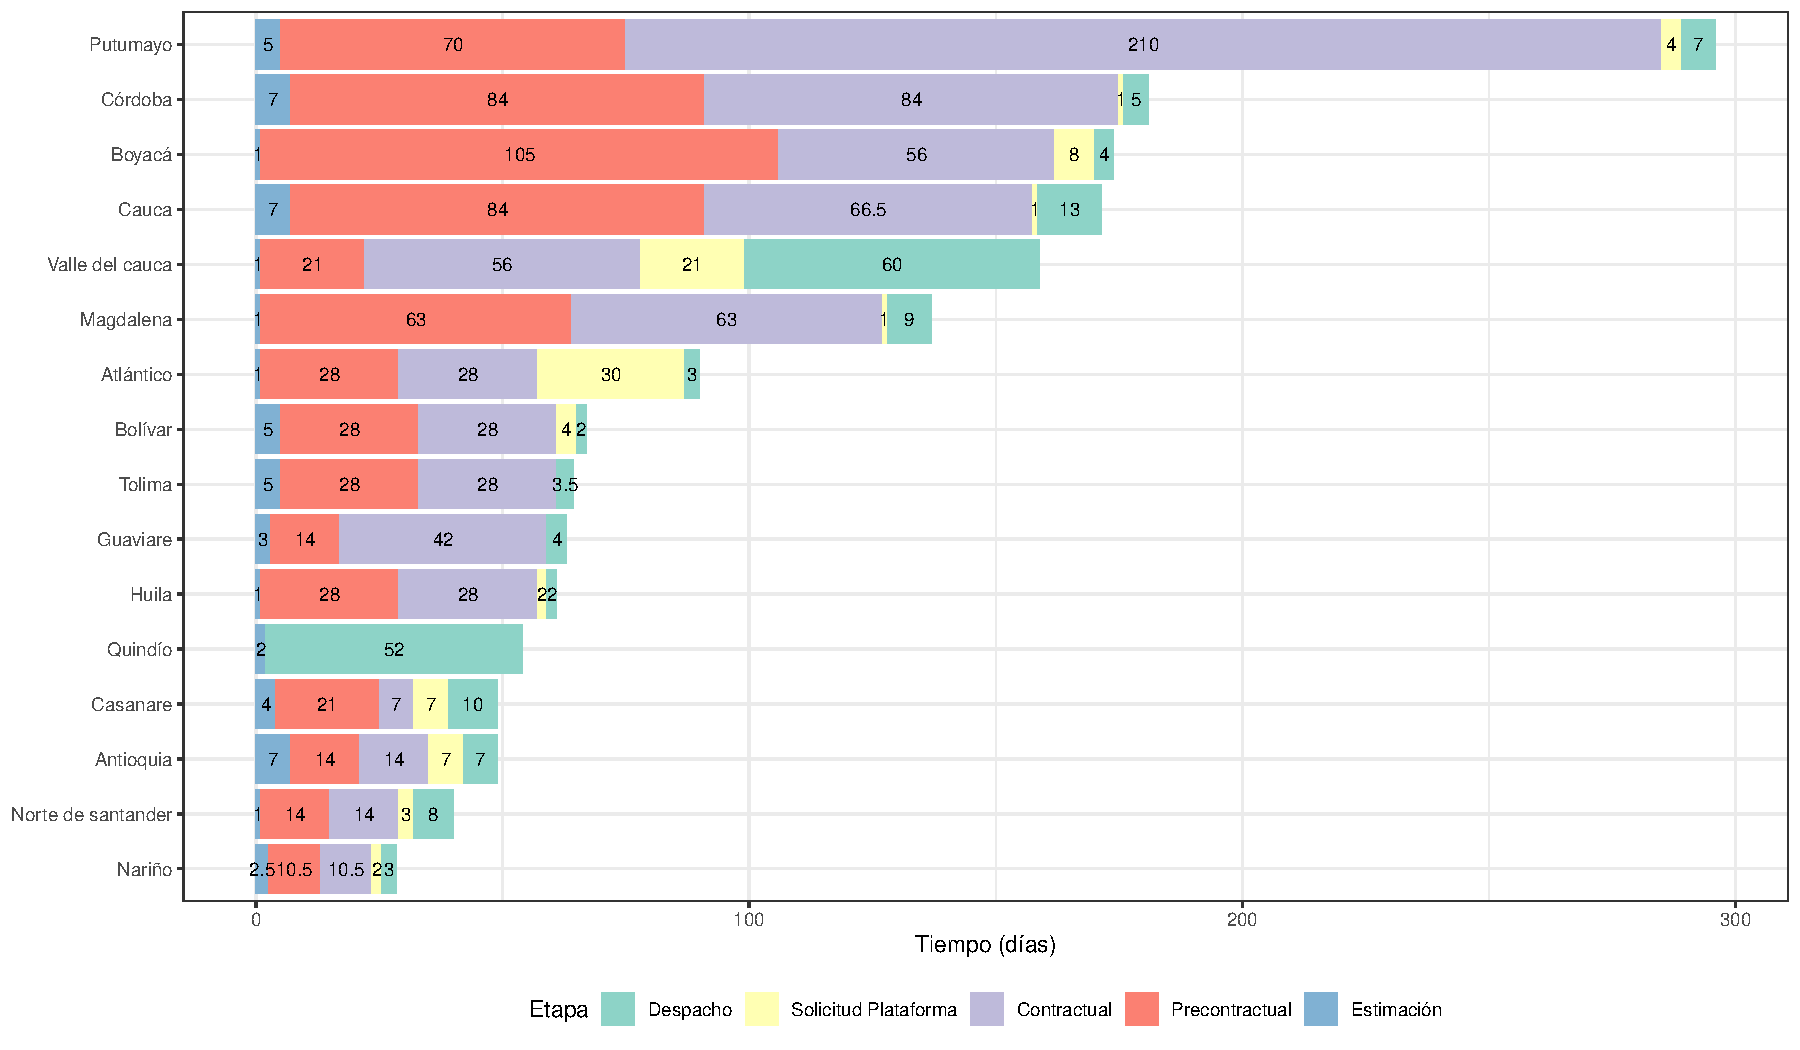
\includegraphics[width=1\linewidth]{InformeFinal_files/figure-latex/EtapasProcesoAdquisicion-1} \caption{Demoras en el proceso de adquisición por departamento}\label{fig:EtapasProcesoAdquisicion}
\end{figure}

Como se identifica en la Figura \ref{fig:EtapasProcesoAdquisicionDetalle}, la gran mayoría de territorios manifiesta que las actividades que más tiempos requieren son las etapas precontractuales y contractuales, esto debido a los requisitos que establece la contratación pública\textsuperscript{\protect\hyperlink{ref-CongresodelaRepublicadeColombia1993}{10},\protect\hyperlink{ref-CongresodelaRepublicadeColombia2007}{11}}. Para que una institución estatal pueda realizar una compra debe tener en cuenta la modalidad de contratación y los documentos exigidos en la misma, p.ej. los estudios previos en los que la entidad debe tener claridad sobre las especificaciones técnicas mínimas del servicio o bien a adquirir (referencia).

\begin{figure}
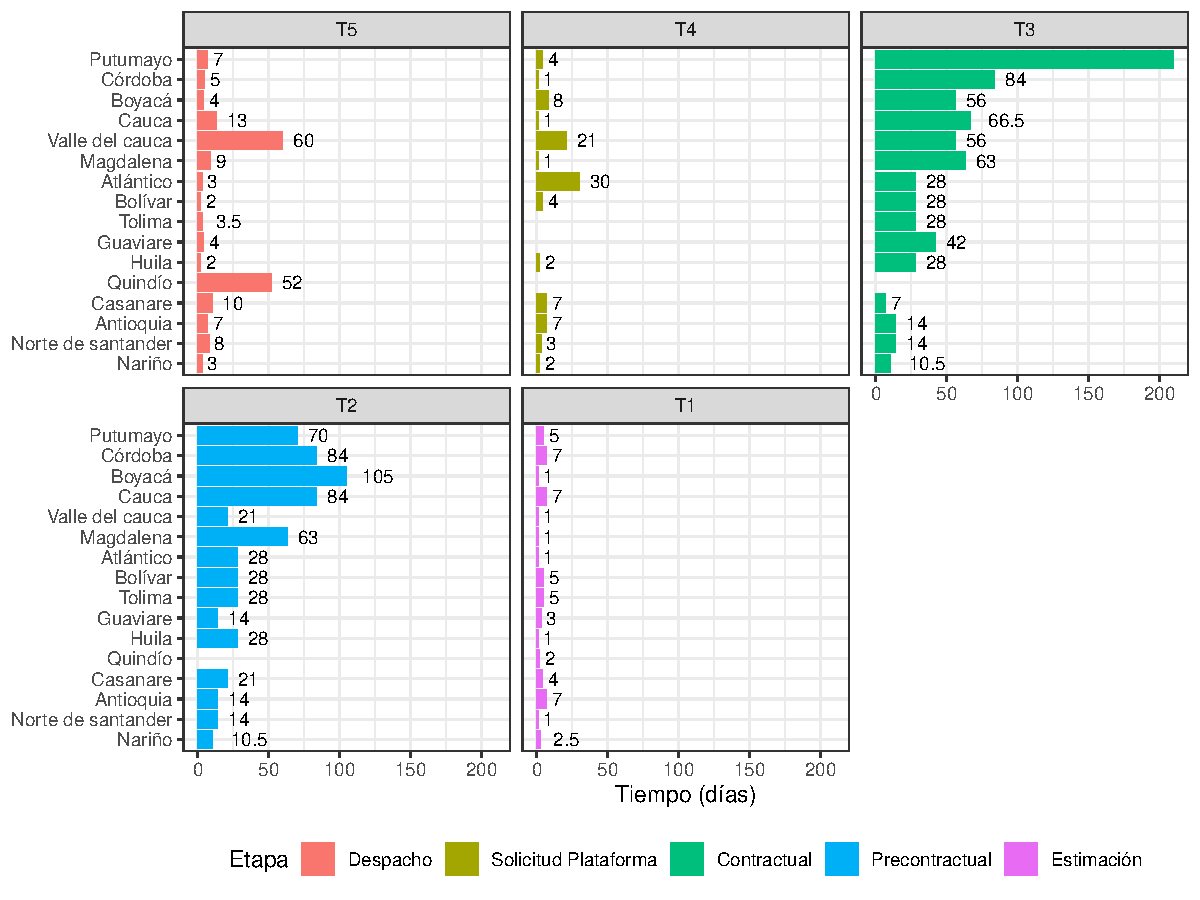
\includegraphics[width=0.85\linewidth]{InformeFinal_files/figure-latex/EtapasProcesoAdquisicionDetalle-1} \caption{Demoras en el proceso de adquisición por departamento (detallado)}\label{fig:EtapasProcesoAdquisicionDetalle}
\end{figure}

Por lo general, la documentación pertinente de la fase precontractual es revisada y corregida en varias ocasiones por diferentes áreas en una misma entidad, lo que conlleva a largos tiempos de espera en la fase precontractual. Estas demoras se dan especialmente cuando el área encargada de aprobar la documentación o de llevar a cabo el proceso contractual no pertenece a la secretaría de salud, como es el caso de Atlántico, pues los funcionarios de otras áreas de las gobernaciones no están inmersos en el contexto de las necesidades de salud pública y específicamente en la importancia que tiene el abastecimiento de MME para la población, por lo que muchas veces el proceso de adquisición de medicamentos queda a merced de la voluntad de otras áreas, propiciando incluso el desabastecimiento en los departamentos.

Por otro lado, el proceso de estimación de compra de MME es uno de los más cortos y por lo general se hace teniendo en cuenta el consumo histórico en el territorio. El consumo histórico de medicamentos no es el único factor para tener en cuenta, es así como en el departamento de Casanare, el FRE además de revisar sus consumos históricos, consulta a sus inscritos la proyección de consumo de cada inscrito, adicionalmente agrega un 20\% a su proyección final para tener un inventario de seguridad que le permita evitar el desabastecimiento.

Por otra parte hay territorios como Guaviare en el que la estimación de compra sólo se hace teniendo en cuenta el consumo histórico y cuidando de no sobrepasar el presupuesto que la gobernación ha asignado para esta tarea. El FRE de Guaviare en comparación con otros territorios es pequeño, evidenciando que las necesidades y capacidades de los FRE son diferentes de acuerdo con el territorio.

Existen casos a exaltar como el FRE de Sucre que, a pesar de tener un tamaño relativamente pequeño a otros en la región, tiene un proceso de estimación de necesidades de MME está altamente estandarizado a través de una herramienta que facilita la toma de decisiones de compra de MME. El FRE afirma que el uso de este manual reduce el tiempo de estimación de compra a una semana, y esto indica que es un proceso eficiente en este departamento.

\hypertarget{traslados-interdepartamentales}{%
\subsection{Traslados interdepartamentales}\label{traslados-interdepartamentales}}

En el traslado interdepartamental de medicamentos se observa que los territorios más descentralizados son los que presentan mayor demora para recibir el traslado de MME, siendo los casos más demorados San Andrés y Amazonas. Como se observa en la Figura \ref{fig:TiemposTranslados} las regiones más afectadas son Amazonía, Orinoquía, Pacífico a excepción del Valle del Cauca y algunos departamentos del Caribe. Sin embargo, el departamento que más demora presenta es San Andrés, pues al estar alejado de la zona continental del país, tiene un tiempo de traslado de medicamentos más largo.

\begin{figure}
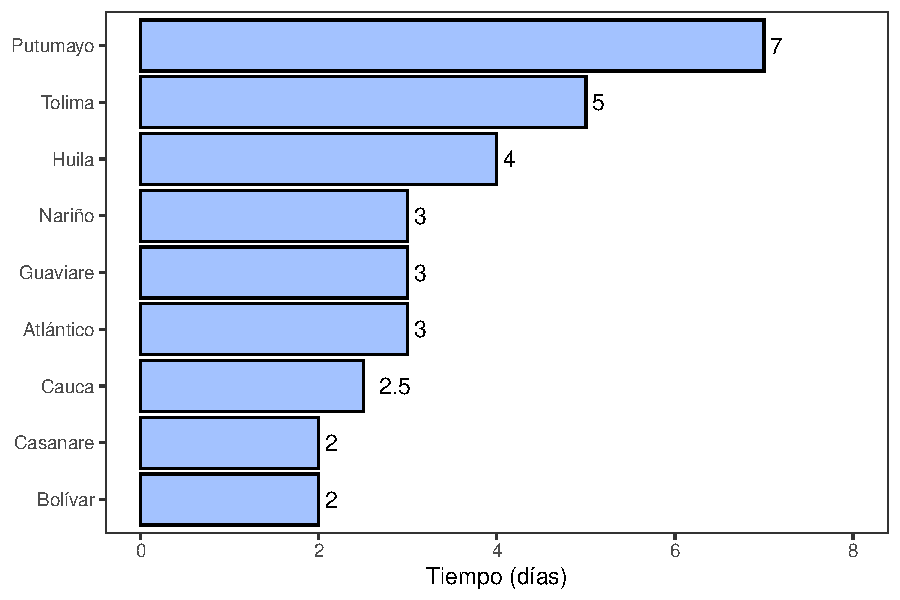
\includegraphics[width=1\linewidth]{InformeFinal_files/figure-latex/TiemposTranslados-1} \caption{Caracterización en demoras de traslados interdepartamentales. Panel A. Gráfico de tiempos de traslados interdepartamentales reportados para los departamentos. Panel B. Mapa de tiempos de traslados interdepartamentales.}\label{fig:TiemposTranslados}
\end{figure}

\hypertarget{plataforma-de-compra-estatal}{%
\subsection{Plataforma de compra estatal}\label{plataforma-de-compra-estatal}}

La plataforma Colombia Compra es el ente rector en materia de contratación pública y desde 2013 se puso en marcha la tienda virtual del Estado colombiano como herramienta en línea del sistema de compra pública. Esta plataforma permite hacer compras a través de acuerdos marco, instrumentos de agregación de demanda y catálogo de bienes de las grandes superficies. En concordancia con lo anterior, Colombia Compra Eficiente dispuso un documento en su plataforma denominado \emph{``Estudios y Documentos Previos de la contratación con el Fondo Nacional de Estupefacientes para la adquisición de Medicamentos de Control Especial de Monopolio del Estado''} donde afirma que se promueve un Instrumento de Agregación de Demanda de Precios para la adquisición de MME mediante contratación directa con el FNE, con el objetivo de aumentar la eficiencia en los procesos de cada FRE y aprovechar las economías a escala. Pese a su implementación y sus objetivos algunos FRE no perciben su uso como una ventaja.

De esta manera los FRE adquieren los MME a través de esta herramienta, por tal motivo se indagó sobre el uso de la plataforma y la opinión que tenían los FRE sobre la misma. Se encuentra que en términos generales (ver la Figura \ref{fig:EtapasProcesoAdquisicionDetalle}), que los FRE consideran que el tiempo invertido en el uso y trámite que se realiza a través de la plataforma, no es tan dispendioso como las etapas precontractuales y contractuales del proceso.

La mayoría de los departamentos hace uso de esta plataforma, encontrándose diferentes percepciones sobre ella. Por ejemplo, el FRE del Cauca indica alta satisfacción con el uso de la plataforma al considerar que es muy organizada, por otra parte el FRE del Valle del Cauca que indica inconformidad en el uso porque consideran que el mismo implica un extenso proceso precontractual y esto puede ser ineficiente y poco intuitivo. El FRE Meta afirma que en la plataforma existen factores que tardan en actualizarse como por ejemplo firmas de la secretaría de salud o incongruencias en el despacho de medicamentos comprados, y el FRE de Santander menciona que los precios en la plataforma suelen encontrarse desactualizados respecto a los del FNE.

Si bien el uso del Instrumento de Agregación de Demanda de precios dispuesto por Colombia Compra Eficiente para la adquisición de MME por parte de los FRE es de obligatoriedad, según la Circular Externa 005 de 2019 emitida por el FNE\textsuperscript{\protect\hyperlink{ref-FNE005-2019}{12}}, no todos llevan a cabo este proceso. Un caso podría ser el FRE Guainía que no ha utilizado la plataforma por falta de conocimiento sobre la misma y tiempo para capacitar a su personal respecto a ello, o el FRE Meta que expresa varias inconformidades sobre el uso de esta.

De otra parte, es necesario mencionar que, si bien casi todos los departamentos hacen uso de la plataforma, este proceso no siempre está a cargo del FRE, como en el caso del departamento del Atlántico, donde el proceso se lleva a través de Secretaría General y por ello su percepción sobre la misma es \emph{``ni conforme ni inconforme''}. Es así como en la Figura \ref{fig:ColombiaCompra} se identifica como la segunda respuesta más frecuente \emph{``Ni conforme ni inconforme''} con el uso de esta plataforma. De otra parte, el FRE Putumayo comenta que el uso de la plataforma depende en gran medida de otras áreas de la gobernación, evidenciando varias dificultades en su uso y aumentando el tiempo en los procesos de contratación.

\begin{figure}
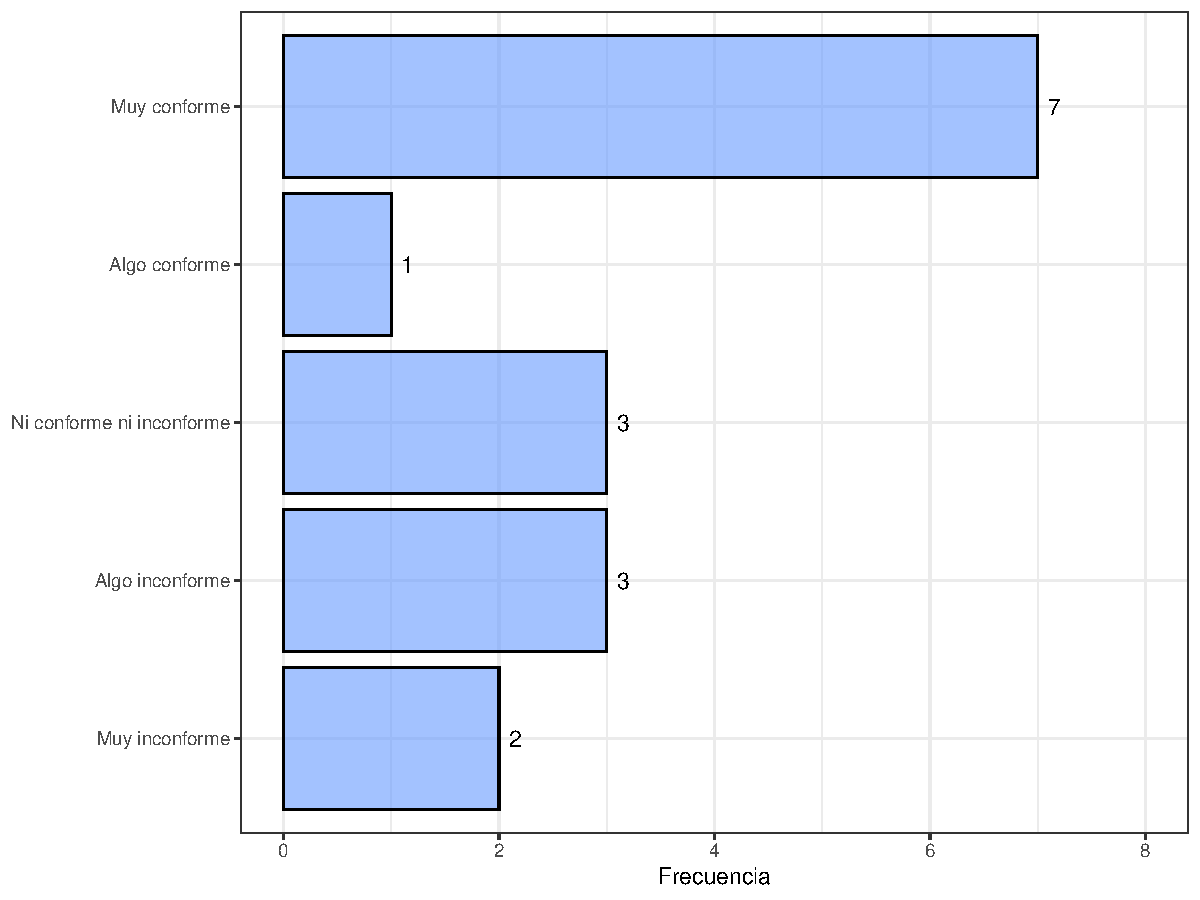
\includegraphics[width=1\linewidth]{InformeFinal_files/figure-latex/ColombiaCompra-1} \caption{Opinión sobre la plataforma Colombia Compra Eficiente}\label{fig:ColombiaCompra}
\end{figure}

En algunos casos, los FRE manifestaron la necesidad de recibir capacitación sobre el uso de esta herramienta, pues el desconocimiento sobre la misma por parte del personal puede ocasionar demoras en el proceso de compra de MME, como ocurre en el caso del FRE Sucre que si bien tienen un método eficiente para realizar la estimación de compra, se ve retrasado en la etapa que implica el uso de esta plataforma.

\hypertarget{comportamiento-de-compra-de-fre}{%
\subsection{Comportamiento de compra de FRE}\label{comportamiento-de-compra-de-fre}}

La frecuencia de las compras de MME al FNE en el año también depende de varios factores como: (a) cantidad requerida de estos bienes por cada departamento, (b) presupuesto asignado por las gobernaciones a los FRE y (c) capacidad de satisfacer la demanda de los medicamentos por parte del FNE (ver Figura \ref{fig:FrecComprasFNR}).

Los FRE con demandas pequeñas de medicamentos, como es el caso de Choco, Guainía y Amazonas, la compra se hace una vez al año, a menos que enfrenten casos de desabastecimiento por causas fortuitas como lo fue la situación de Emergencia Sanitaria por la pandemia de coronavirus. Los departamentos con mayor población y necesidad de medicamentos se ven en la obligación de realizar varias compras en el año como es el caso del departamento de Antioquia cuya intención es realizar compras proyectando un abastecimiento de tres meses, sin embargo, manifiesta que el proceso se ve entorpecido por el bajo nivel de servicio relacionado a la disponibilidad de medicamentos en el FNE que le permitan satisfacer su demanda. Se presenta un caso similar para el FRE Santander, donde también afirman que la disponibilidad de medicamentos por parte del FNE es muy poca para cubrir la demanda de su departamento, por lo que obligatoriamente deben autorizar a las IPS y demás a hacer compras directas al FNE.

Por otra parte, hay departamentos donde la frecuencia de las compras y las cantidades de esta depende del presupuesto asignado por la gobernación, como es el caso de Guainía y Putumayo, este último indica que la demanda de MME en su territorio es más alta de la que se puede cubrir por limitaciones presupuestales.

Por su parte, otros territorios no pueden realizar las compras con las frecuencias que requieren por problemas administrativos o económicos de alguna índole que corresponden a la gobernación, como han manifestado los FRE de San Andrés, Atlántico y Huila.

\begin{figure}
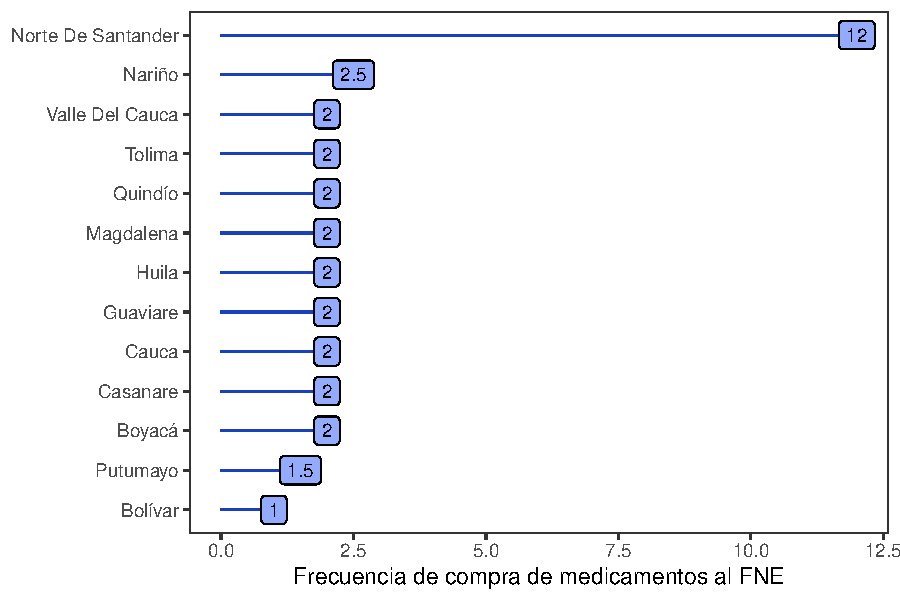
\includegraphics[width=0.9\linewidth]{InformeFinal_files/figure-latex/FrecComprasFNR-1} \caption{Frecuencia de compras de medicamentos por año al FNE}\label{fig:FrecComprasFNR}
\end{figure}

La venta de MME a instituciones en los departamentos se da según lo establecido por cada FRE y las necesidades de cada departamento, p.ej. en el departamento de Vaupés cuyo abastecimiento se enfoca en satisfacer la demanda del Hospital, no se realiza venta a otras IPS y por lo tanto ni si quiera tienen necesidad de almacenar los medicamentos en el FRE, las compras se destinan inmediatamente al Hospital. Se presenta un caso diferente en departamentos con mayor población y necesidad de medicamentos como Risaralda donde la venta de MME es frecuente, sin embargo, se ha establecido a las IPS que deben proyectar sus necesidades mensualmente.

\begin{figure}
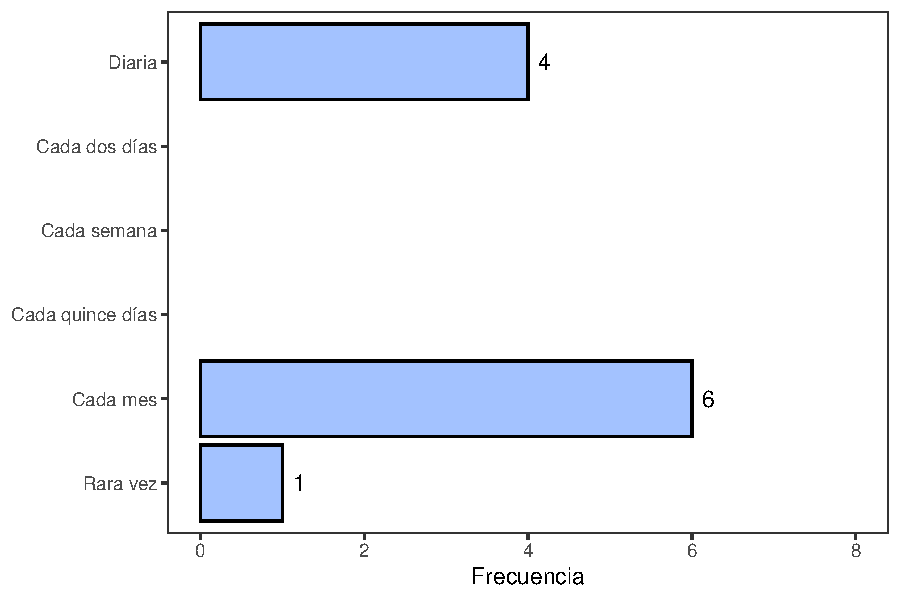
\includegraphics[width=0.85\linewidth]{InformeFinal_files/figure-latex/FrecVentaInstituciones-1} \caption{Frecuencia de venta de MME a instituciones en el departamento}\label{fig:FrecVentaInstituciones}
\end{figure}

En el departamento del Atlántico antes de la pandemia la venta de medicamentos se hacía diariamente, sin embargo, por la contingencia en salud se decidió que solo se despachan medicamentos dos días a la semana. Otro departamento que hace venta diaria de MME es Choco y afirma que las necesidades de MME pueden variar en el departamento gracias al traslado no esperado de pacientes de zonas muy distantes a las capitales de los departamentos de Antioquia y Valle del Cauca.

\hypertarget{recepciuxf3n-de-medicamentos}{%
\section{Recepción de medicamentos}\label{recepciuxf3n-de-medicamentos}}

\maxdeadcycles=1000

\begin{figure}
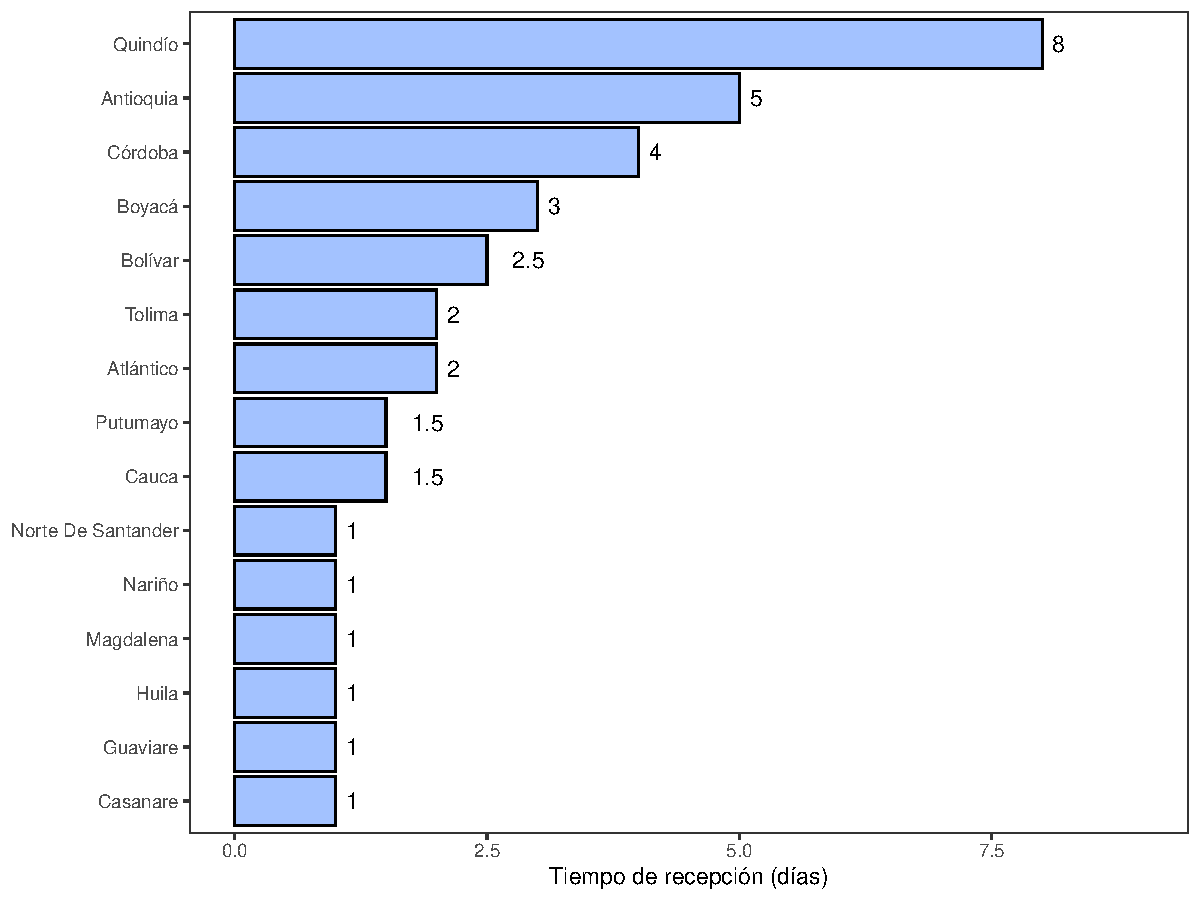
\includegraphics[width=0.85\linewidth]{InformeFinal_files/figure-latex/TiemposRecepcionAlmacenamiento-1} \caption{Tiempos en la recepción técnica y almacenamiento de MME}\label{fig:TiemposRecepcionAlmacenamiento}
\end{figure}

\begin{figure}
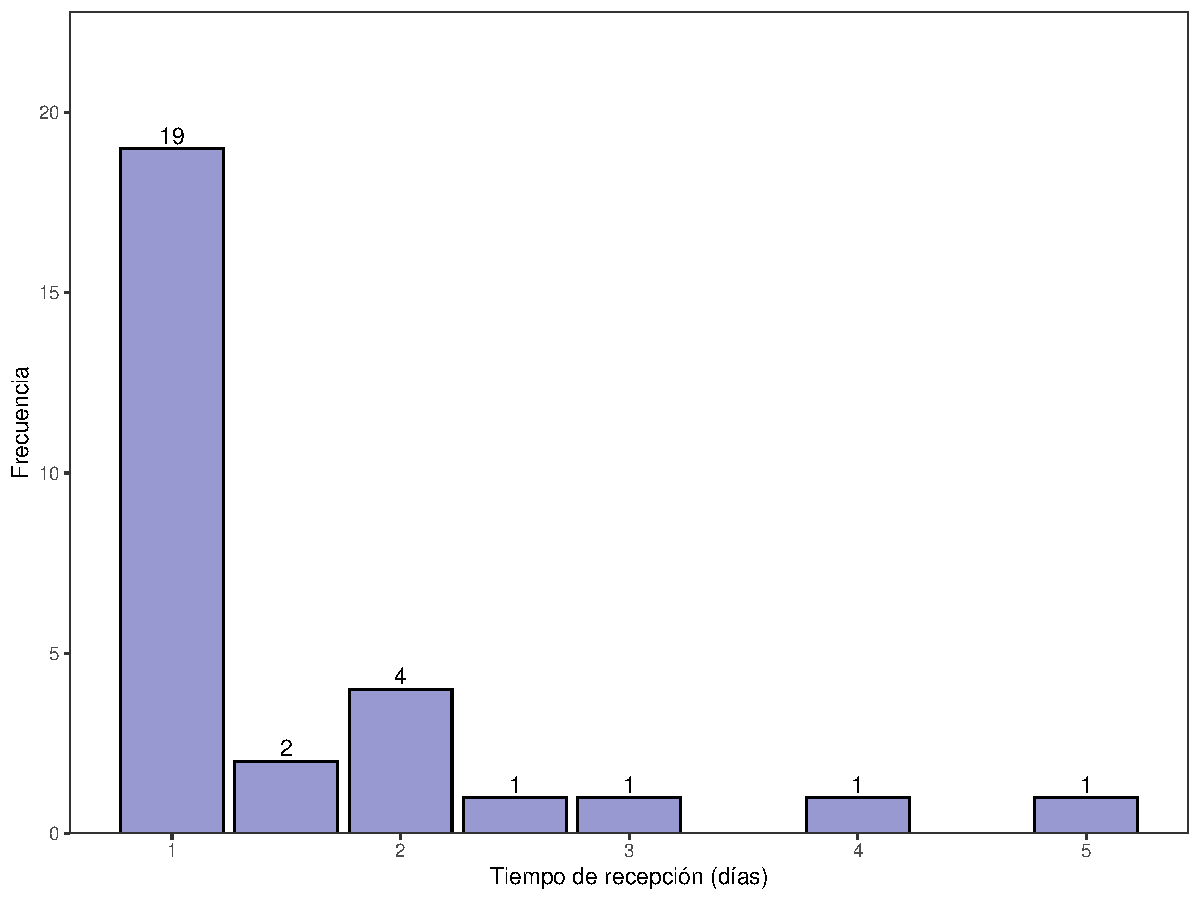
\includegraphics[width=0.85\linewidth]{InformeFinal_files/figure-latex/TiemposRecepcionAlmacenamientob-1} \caption{Tiempos en la recepción técnica y almacenamiento de MME}\label{fig:TiemposRecepcionAlmacenamientob}
\end{figure}

\begin{figure}
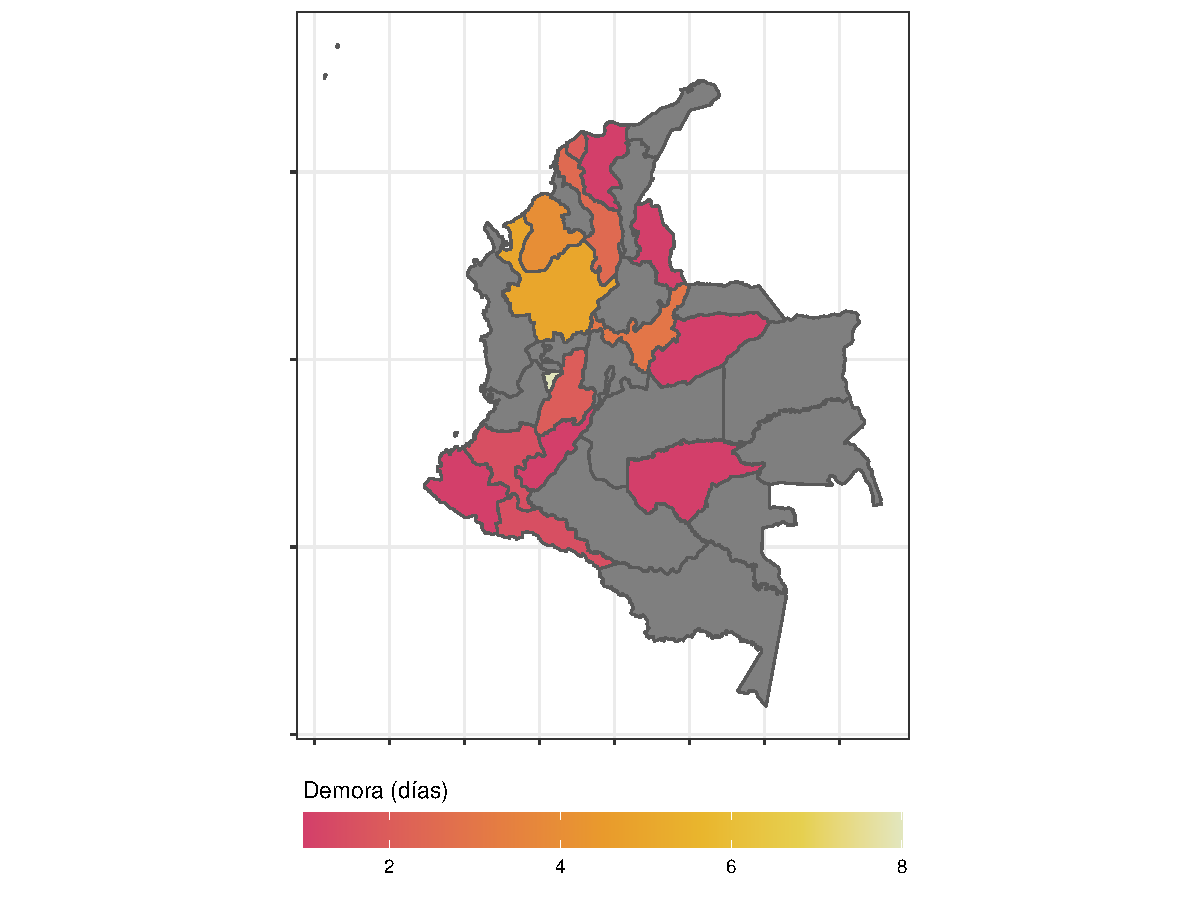
\includegraphics[width=0.85\linewidth]{InformeFinal_files/figure-latex/TiemposRecepcionAlmacenamientoMapa-1} \caption{Tiempos en la recepción técnica y almacenamiento de MME (mapa)}\label{fig:TiemposRecepcionAlmacenamientoMapa}
\end{figure}

\begin{figure}
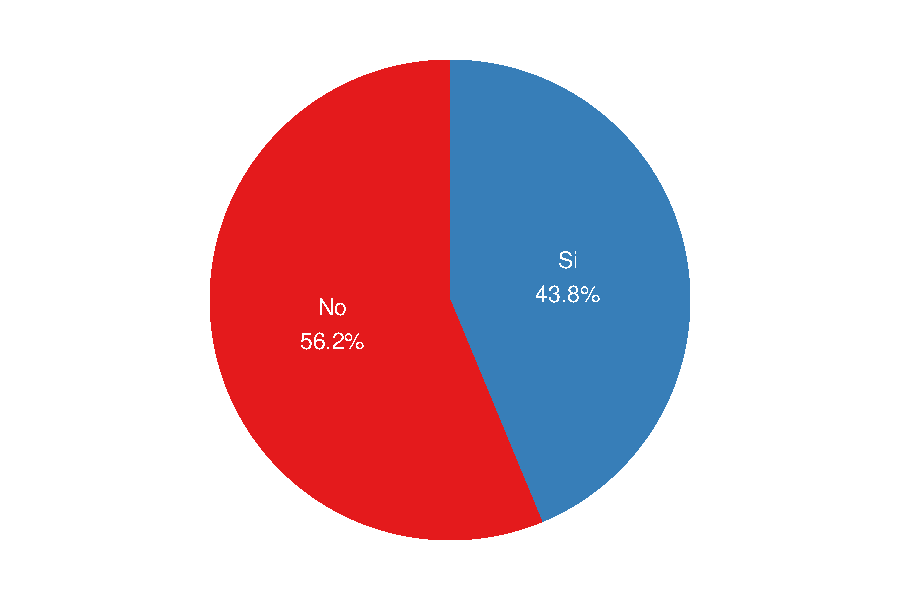
\includegraphics[width=0.85\linewidth]{InformeFinal_files/figure-latex/UsoNivelesSeguridad-1} \caption{Uso de niveles de seguridad del inventarios}\label{fig:UsoNivelesSeguridad}
\end{figure}

\hypertarget{almacenamiento}{%
\section{Almacenamiento}\label{almacenamiento}}

\hypertarget{medidas-de-seguridad-para-el-almacenamiento}{%
\subsection{Medidas de seguridad para el almacenamiento}\label{medidas-de-seguridad-para-el-almacenamiento}}

\maxdeadcycles=1000

En la Figura \ref{fig:MedidasSeguridadAlmacenamientoMME} se listan las medidas de seguridad adoptadas por los FRE para disminuir la posibilidad de robo con fines de desvío de los MME. Las medidas más adoptadas por parte de los FRE consisten en: (a) el acceso de seguridad restringido a cierto personal (con respuesta afirmativa por parte de 18 de 26 FRE), seguido de (b) gabinetes con llaves simple (en 14 de 26 FRE), (c) almacenamiento en oficina privada (14 de 26 FRE responden que lo aplican), (d) inventarios físicos diarios, y (e) protección en gabinetes hechos de materiales resistentes.

\begin{figure}
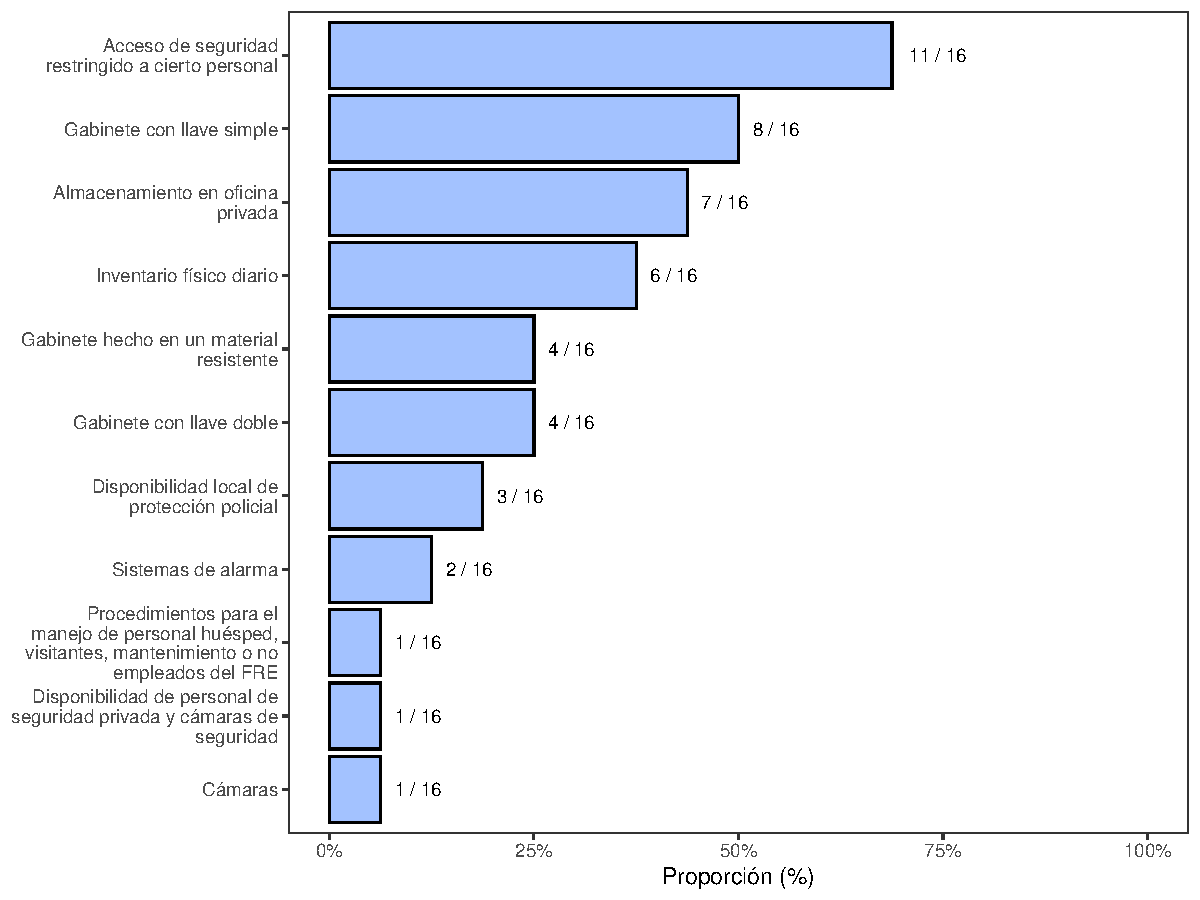
\includegraphics[width=0.9\linewidth]{InformeFinal_files/figure-latex/MedidasSeguridadAlmacenamientoMME-1} \caption{Medidas de seguridad en el almacenamiento de MME}\label{fig:MedidasSeguridadAlmacenamientoMME}
\end{figure}

El departamento que reporta la mayor cantidad de medidas de seguridad es César con 7 medidas como: (a) acceso de seguridad restringido a cierto personal, (b) procedimientos para el manejo de personal huésped, (c) visitantes, (d) mantenimiento o no empleados del FRE, (e) almacenamiento en oficina privada, (f) inventario físico diario, y (g) Disponibilidad local de protección policial. Entre los FRE con mayor número de medidas de seguridad reportadas se tiene Casanare (con 6 medidas reportadas), y Córdoba, Antioquia, Norte de Santander, Valle del Cauca, Guaviare y Risaralda con 5 medidas reportadas. Los FRE de Atlántico, Magdalena, Huila, Quindío, y Amazonas sólo reportan una medida de seguridad.

Sólo los FRE de Valle del Cauca y Córdoba reportan la existencia de un sistema de monitoreo por cámaras para los medicamentos. Sólo los FRE de Córdoba y Vichada reportan la presencia de seguridad privada como medida de seguridad para los FRE. Se recomienda la adopción de una o varias medidas de seguridad por parte de los FRE frente a posibles robos con intenciones de desvío o tráfico de medicamentos MME.

\hypertarget{revisiuxf3n-de-condiciones-ambientales}{%
\subsection{Revisión de condiciones ambientales}\label{revisiuxf3n-de-condiciones-ambientales}}

En la Figura \ref{fig:FrecRevCondiciones} se muestra la frecuencia de revisión de condiciones ambientales en el almacenamiento de MME. Se tienen que la práctica más frecuente en los FRE es la realización de verificación de condiciones ambientales por lo menos dos veces al día. Sólo algunos FRE afirman que no hacen revisión de condiciones ambientales como Bolívar, Sucre, Chocó, Norte de Santander, Amazonas y Vichada.

\begin{figure}
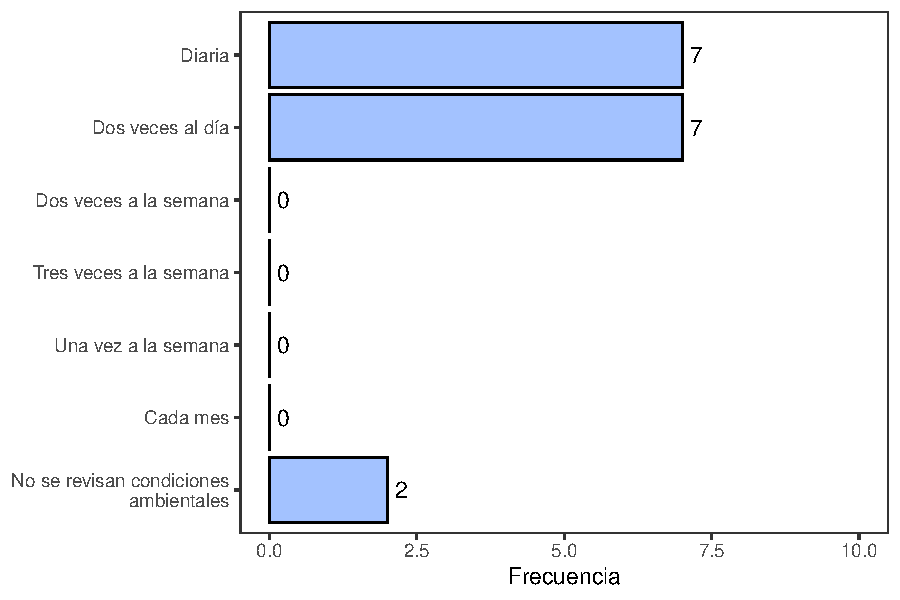
\includegraphics[width=0.85\linewidth]{InformeFinal_files/figure-latex/FrecRevCondiciones-1} \caption{Frecuencia de revisión de condiciones ambientales}\label{fig:FrecRevCondiciones}
\end{figure}

En el panel izquierdo de la Figura \ref{fig:MetodosSeguimientoControlAmbiental} se presentan los métodos o tecnologías utilizadas en la monitorización de los medicamentos. En la Figura \ref{fig:MetodosSeguimientoControlAmbiental} se observa que al menos 25 de 30 fondos rotatorios cuentan con un termohigrómetro para la evaluación de condiciones ambientales. La práctica de diligenciar registros cuenta con una menor adopción por parte de los fondos rotatorios, se tiene que 7 y 4 de los fondos rotatorios realiza el diligenciamiento de estos formatos de manera manual y electrónica de manera respectiva.

\begin{figure}[t]
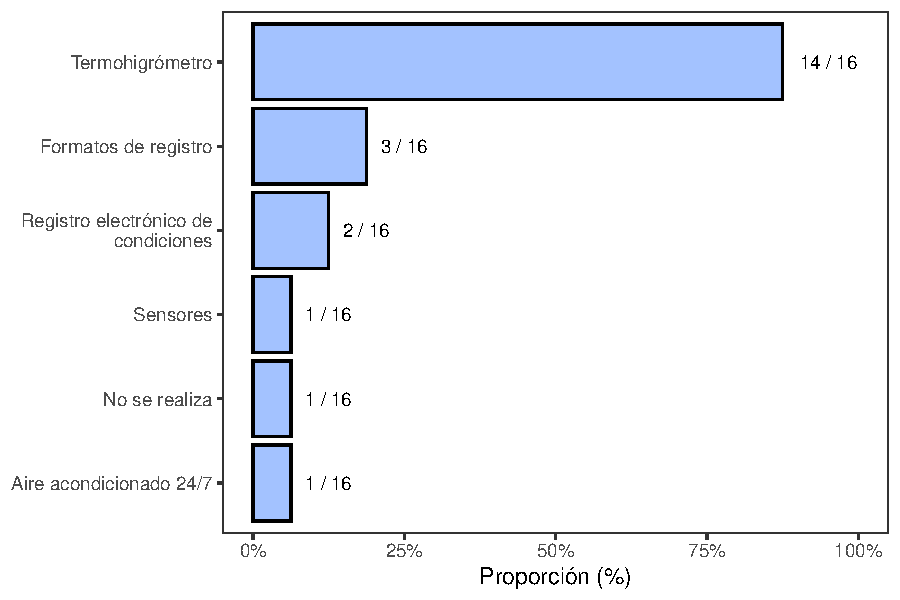
\includegraphics[width=1\linewidth]{InformeFinal_files/figure-latex/MetodosSeguimientoControlAmbiental-1} \caption{(A) Tecnologías de control y seguimiento de condiciones ambientales y (B) Frecuencia de calibración y mantenimiento de equipos de seguimiento ambiental}\label{fig:MetodosSeguimientoControlAmbiental}
\end{figure}

En sólo dos FRE (Chocó y Norte de Santander) se reporta el uso de aire acondicionado como una medida para el seguimiento de condiciones ambientales. En el panel derecho de la Figura \ref{fig:MetodosSeguimientoControlAmbiental} se tiene que la práctica más común es realizar la calibración de los equipos de monitoreo por lo menos una vez al año, y hasta en 11 se tiene que no hay un procedimiento de calibración de los equipos. La mayoría de departamentos que no realizan el proceso de calibración se encuentran en la región central.

\hypertarget{espacio-de-almacenamiento}{%
\subsection{Espacio de almacenamiento}\label{espacio-de-almacenamiento}}

En la Figura \ref{fig:ProductosCompartidos1} se muestra la frecuencia de varias categorías de productos con los cuales se comparten los MME en el almacén de los FRE. Se tiene que en casi la mitad de los FRE se comparten los MME con medicamentos de salud pública, en 7 de 30 casos se reporta la utilización del espacio en conjunto con papelería (7/30) o recetarios oficiales (3/30). Algunos FRE tienen otros items como vacunas, medicamentos de carros de paro y medicamentos incautados. En 9 de 30 casos se tiene que el FRE tiene un espacio dedicado únicamente a MME.

\begin{figure}
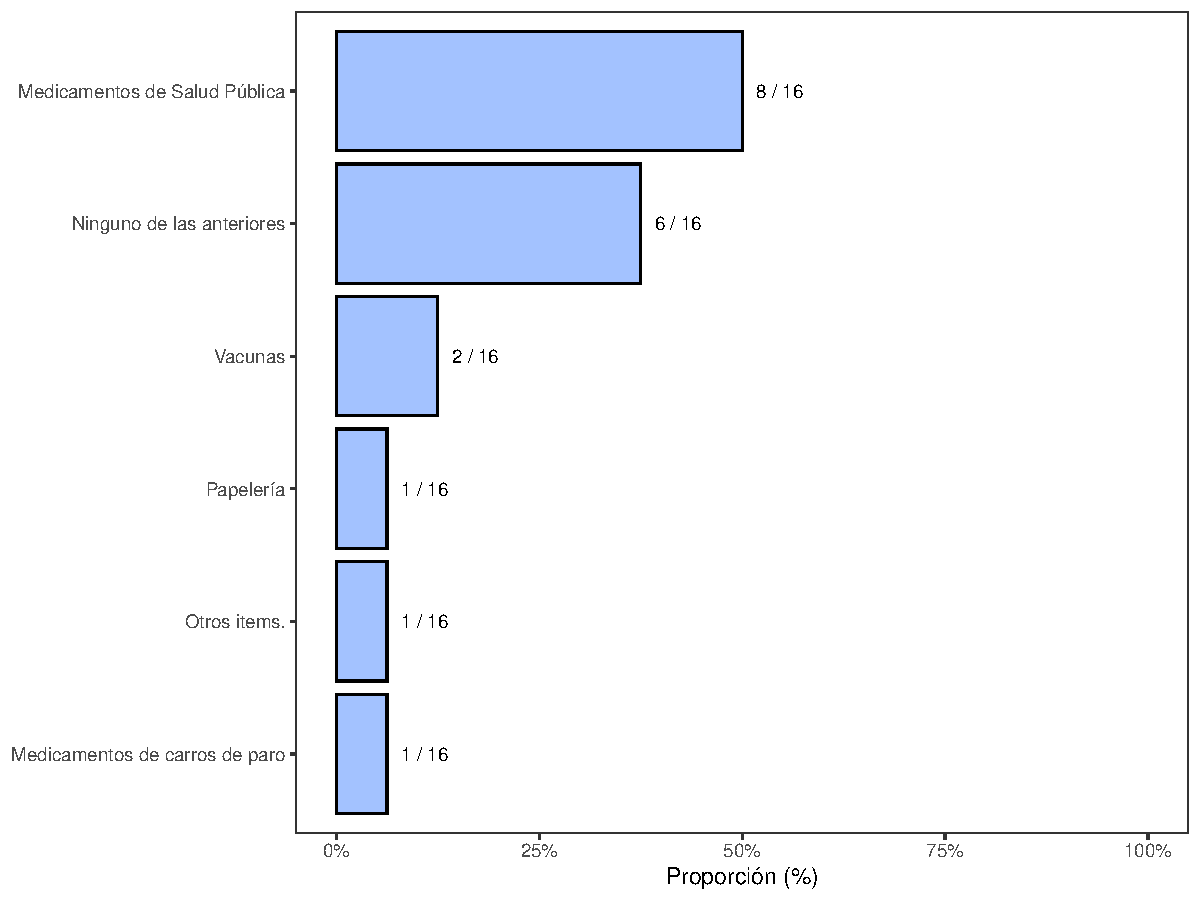
\includegraphics[width=0.85\linewidth]{InformeFinal_files/figure-latex/ProductosCompartidos1-1} \caption{Productos compartidos en el almacén de MME}\label{fig:ProductosCompartidos1}
\end{figure}

En la Figura \ref{fig:PropOcupacionAlmacen} se tiene una estimación del promedio de ocupación de medicamentos MME en los almacenes frente a otros productos. Se tiene que la práctica más común es la utilización de un espacio destinado exclusivo para estos medicamentos y esto se da en 12 FREs.

\begin{figure}
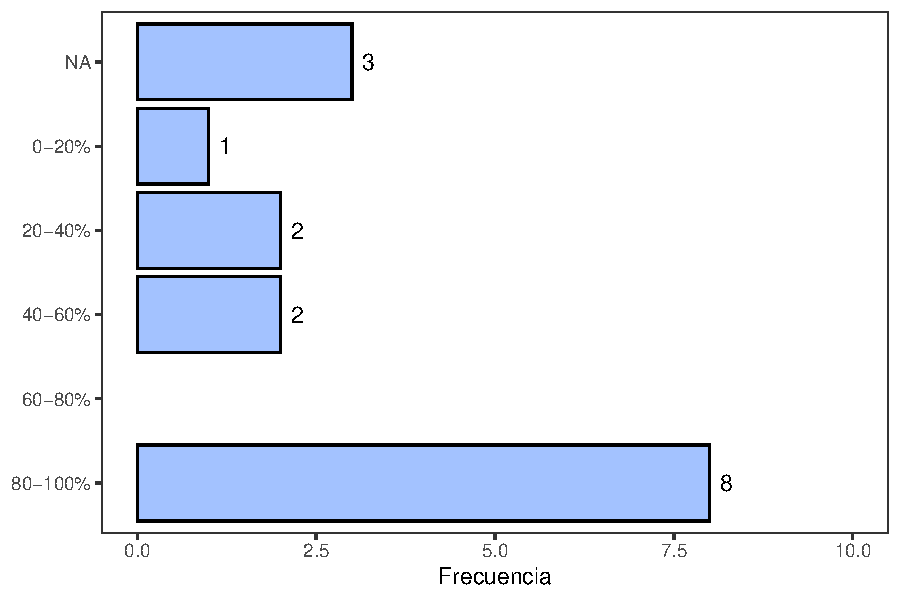
\includegraphics[width=0.85\linewidth]{InformeFinal_files/figure-latex/PropOcupacionAlmacen-1} \caption{Ocupación promedio del MME frente a otros medicamentos o ítems almacenados en el FRE}\label{fig:PropOcupacionAlmacen}
\end{figure}

Se considera que existen dos tipos de métodos de control de inventario conocidos como sistemas perpetuos o periódicos\textsuperscript{\protect\hyperlink{ref-Silver2017}{13}}.
En la Figura \ref{fig:FrecControlExistencias} se tiene una caracterización de la frecuencia de control de existencias de los MME. En la mayoría de los FRE se realiza esta verificación de manera mensual, o de forma diaria. La frecuencia de monitoreo de existencias parece estar relacionada con el nivel medio de inventario.

\begin{figure}
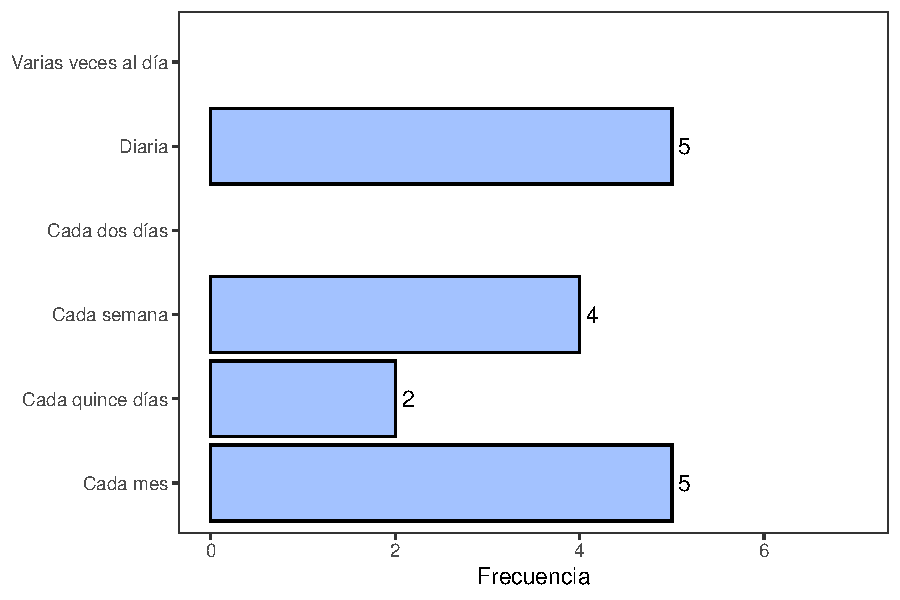
\includegraphics[width=1\linewidth]{InformeFinal_files/figure-latex/FrecControlExistencias-1} \caption{Frecuencia del control de existencias de medicamentos MME}\label{fig:FrecControlExistencias}
\end{figure}

Entre los FRE que afirman realizar el monitoreo de niveles de inventarios de forma diaria se encuentran Antioquia, Córdoba, Bolívar, San Andrés, Casanare, Meta y Caldas. El FRE de Cesar afirma realizar el control de existencias varias veces al día. Los FRE que realizan monitoreo cada mes parecen encontrarse en las regiones más periféricas del territorio, y esto se podría deber a la presencia de niveles de inventario promedio bajos.

\hypertarget{control-de-fechas-de-vencimiento}{%
\subsection{Control de fechas de vencimiento}\label{control-de-fechas-de-vencimiento}}

De acuerdo a la Resolución 1403 de 2007 del MSPS\textsuperscript{\protect\hyperlink{ref-MinisteriodeSaludyProteccionSocial2007}{14}}, el control de fechas de vencimiento es un procedimiento importante enmarcado en el proceso de Recepción y Almacenamiento de Medicamentos y Dispositivos Médicos dentro del Modelo de Gestión del Servicio Farmacéutico. Los servicios farmacéuticos deben contar con criterios procedimientos y recursos que le permitan verificar y recursos que permitan verificar continuamente la fecha de vencimiento de los medicamentos\textsuperscript{\protect\hyperlink{ref-MinisteriodeSaludyProteccionSocial2007}{14}}.

Entre estos recursos se encuentra la \emph{semaforización}, que es una herramienta que permite identificar y determinar en el momento oportuno que medicamentos están próximos a vencer. De forma común, esta herramienta se aplica mediante la rotulación de las unidades con colores de los medicamentos de acuerdo al tiempo esperado hasta la fecha de vencimiento\textsuperscript{\protect\hyperlink{ref-HernandezVera2017}{15}}. La semaforización también se podría aplicar mediante sistemas de alertas electrónica.

La adopción de esta práctica sólo se ha realizado en 40\% de los FRE. Esta práctica se lleva a cabo teniendo en cuenta tres colores:

\begin{itemize}
\tightlist
\item
  Rojo: medicamento que se encuentra próximo a vencer.
\item
  Amarillo: medicamento que se encuentra en riesgo moderado de vencimiento.
\item
  Verde: medicamento que no tiene riesgo de vencimiento. En ocasiones, no se genera ningún tipo de alerta cuando el producto está en esta condición.
\end{itemize}

Los umbrales adoptados por la mayoría de las entidades ha sido \texttt{6\textbar{}12} que indica colocar una etiqueta roja sí el medicamento se encuentra a 6 meses de vencerse, y una etiqueta amarilla sí el medicamento se encuentra a 12 meses de vencerse. Algunos FRE también tienen umbrales de \texttt{3\textbar{}6} meses para el proceso de semaforización.

En la Figura \ref{fig:CasosVencimiento1} se observa que el 71\% de los FRE han presentado casos de medicamentos vencidos lo que constituye a 22 de 31 FRE existentes en el país, y esto indica que los vencimientos son una situación frecuente para los FRE.

\begin{figure}
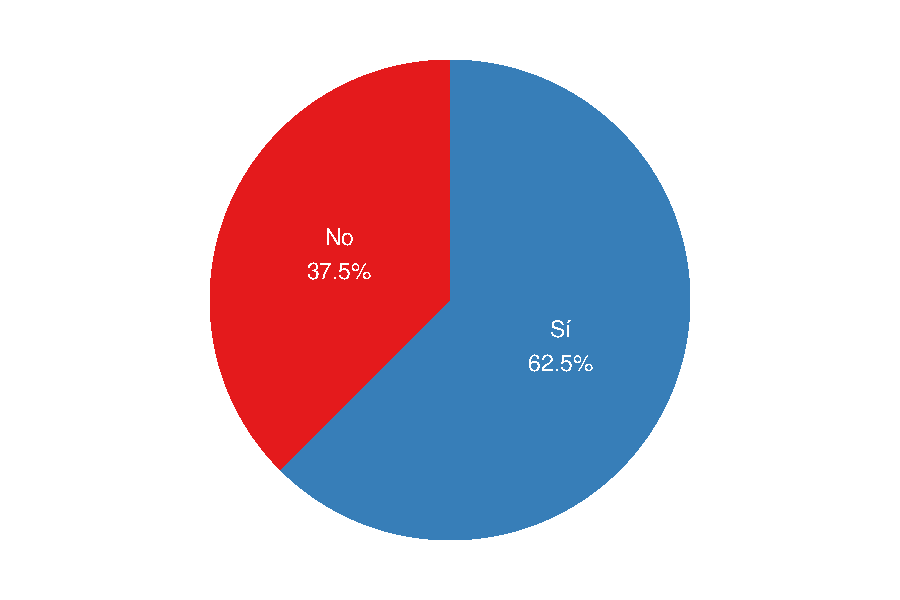
\includegraphics[width=0.85\linewidth]{InformeFinal_files/figure-latex/CasosVencimiento1-1} \caption{Presentación de casos de vencimiento de MME}\label{fig:CasosVencimiento1}
\end{figure}

En la Figura \ref{fig:CasosVencimiento2} se muestran los medicamentos más involucrados en casos de vencimientos. En primer lugar, se tiene al Metilfenidato Tableta x 10 mg ya que 13 de los 31 FRE han presentado vencimientos relacionados a este producto. La razón para estos vencimientos podría deberse a varios factores como:

\begin{itemize}
\tightlist
\item
  El producto cuenta con una vida útil de 18 meses.
\item
  Este medicamento es importado y en ocasiones la casa matriz entrega el producto con una vida útil efectiva menor a los 18 meses mencionados.- Debido a la emergencia sanitaria producida por el coronavirus se ha presentado una contracción importante de la demanda que se encuentra posiblemente relacionada a los cambios en la movilidad de los ciudadanos y las restricciones de presencialidad en instituciones escolares.
\end{itemize}

El segundo medicamento más involucrado en casos de vencimiento es Primidona Tableta x 250 mg debido a que 4 de los 31 FRE reportan casos de vencimientos, seguido de los vencimientos de Meperidina de 100mg/2mL, Fenobarbital Solución inyectable x 40 mg/mL y Fenobarbital Solución inyectable x 200 mg/mL que fueron reportados por 3 de 31 FREs a nivel nacional que se puede explicar debido a que son productos de baja rotación, y es posible que los FRE no hayan recibido una adecuada asistencia por parte del FNE para el manejo de ítems de este tipo.

\begin{figure}
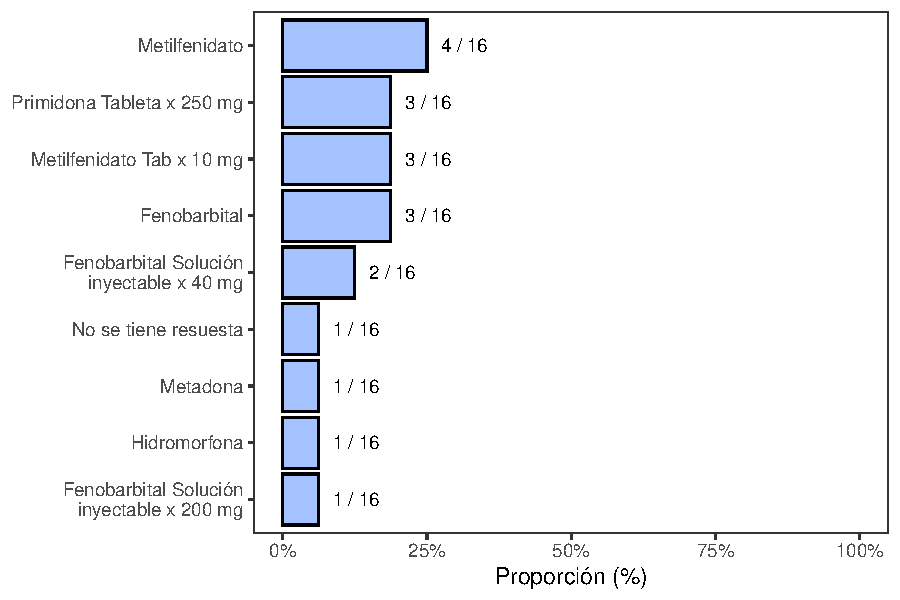
\includegraphics[width=0.85\linewidth]{InformeFinal_files/figure-latex/CasosVencimiento2-1} \caption{Medicamentos implicados en casos de vencimiento de MME}\label{fig:CasosVencimiento2}
\end{figure}

\hypertarget{transporte}{%
\subsection{Transporte}\label{transporte}}

El transporte de medicamentos por parte del FNE, es un proceso importante dentro de la cadena de suministro de MME. Los costos de transporte de medicamentos por parte del FNE están cubiertos dentro del precio de los MME. El FNE contrata a una empresa especializada en distribución logística de mercancías y bienes para la entrega del producto a nivel nacional.

En la Figura \ref{fig:TransporteProductos} se tiene una descripción de la opinión del servicio de distribución por parte del FNE. Se tiene que las opiniones se encuentran divididas con algunas respuestas positivas (66.6\%) y otras negativas (33.3\%).

\begin{figure}
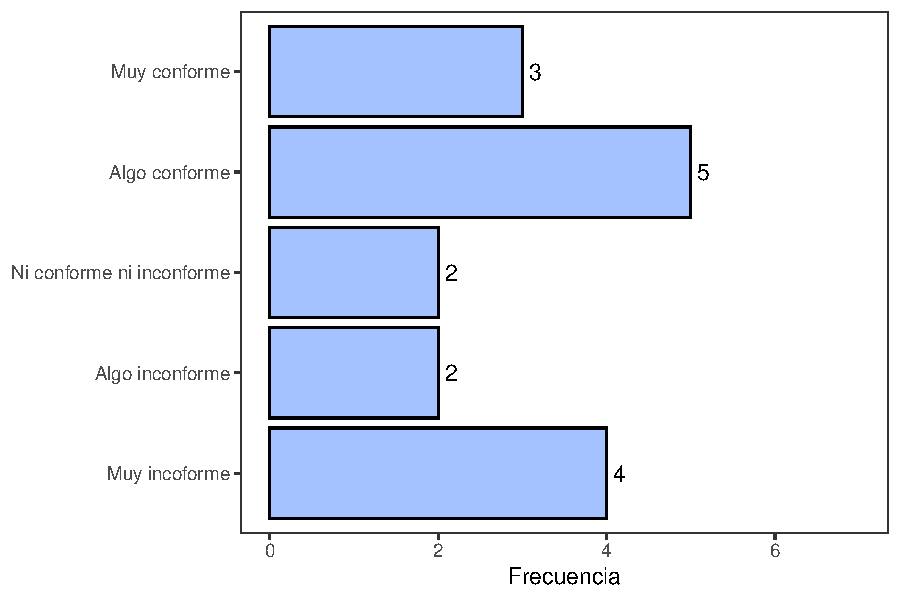
\includegraphics[width=0.85\linewidth]{InformeFinal_files/figure-latex/TransporteProductos-1} \caption{Opinión del servicio de la distribución de los medicamentos MME}\label{fig:TransporteProductos}
\end{figure}

En cuanto a las opiniones negativas se tiene como principal queja a las averías en los productos causadas por el transporte. Se tienen también quejas relacionadas con (i) problemas en el enrutamiento de los envíos, (ii) demoras, (iii) disposición de los medicamentos en la entrada de las secretarías sin entregarlos de forma directa a los encargados, (iv) falta de cobertura en todo el territorio y (v) condiciones de almacenamiento inadecuadas.

\begin{quote}
\emph{``Problemas de embalaje y muchos problemas de averías''}
\end{quote}

Los problemas en el transporte de medicamentos han generado inconvenientes relacionados a sobrecostos en este mismo rubro, de manera que algunos FRE han tenido que recurrir a otros convenios, por ejemplo como aquellos utilizados por medicamentos de salud pública.

En cuanto a las respuestas positivas se tiene que la mayoría de los FRE que responden de esta manera no han tenido inconvenientes con la entrega de los productos. Algunos de estos FRE manifiestan que la empresa hace llegar el producto dentro de 5 días después del despacho, así mismo que los medicamentos llegan en buenas condiciones y que no se han tenido problemas. Sólo algunos de los FRE no tienen registros de inconvenientes con el transportador previamente. Un ejemplo de respuesta positiva ha sido:

\begin{quote}
\emph{``No hemos tenido inconvenientes con el transporte de MME. Cuando surge un caso de producto no conforme, el FNE siempre responde y efectúa la devolución de estos productos con averías.''}
\end{quote}

Se tiene que pese a que más del 50\% de los respondientes de la encuesta tienen una opinión positiva del transporte de los medicamentos, casi 1 de cada 3 FRE no están satisfechos con el servicio. El alto grado de insatisfacción y las causas que justifican la opinión se deben tener en cuenta como aspectos para el mejoramiento del proceso.

\hypertarget{precio-de-medicamentos}{%
\section{Precio de medicamentos}\label{precio-de-medicamentos}}

\maxdeadcycles=1000

En la gestión de operaciones de distribución de MME por parte del FNE, se consideran dos canales de distribución principales los cuales son: (i) canal de distribución a FRE y (ii) canal de distribución mediante compra directa. Se considera que el canal de compra directa constituye una excepción, en los casos en donde no existe un Fondo Rotatorio que realice la distribución en un departamento determinado. Debido a esto, se debe considerar un precio de venta mayor en la utilización del canal de compra directa, y en el caso de MME se realiza la estimación del precio de venta a FRE y se adiciona un margen del 12\% para las operaciones en canal de compra directa.

En la Figura \ref{fig:precioVentasDepartamentos} se observa una comparación de los precios de ventas reportados como oficiales por los FRE en sus respectivos departamentos para la vigencia 2021. El precio se muestra para cada medicamento en una escala de color diferente en pesos colombianos. En la figura se puede observar que los medicamentos más costosos corresponden a Metilfenidato 36 mg (entre \(\$300.000\) y \(\$900.000\)) y Metilfenidato 36 mg (entre \(\$200.000\) y \(\$600.000\) pesos).

\begin{figure}[t!]
\includegraphics[width=1\linewidth]{InformeFinal_files/figure-latex/precioVentasDepartamentos-1} \caption{Precio de venta de medicamentos en los FRE}\label{fig:precioVentasDepartamentos}
\end{figure}

En la línea de anticonvulsivantes se tiene que el medicamento más costoso es Fenobarbital 200 mg/mL con precios entre \(\$75,000\) a \(\$150,000\), mientras que en la línea de narcóticos se tiene al producto importado de Metadona tabletas 40mg como el más costoso (con precios que rondan \(\$100,000\) y \(\$200,000\)). Se tiene algunos departamentos con un color gris, lo que indicaría que el medicamento no hace parte del portafolio de MME que es distribuido en el departamento. Por otra parte, se tienen departamentos con un color de relleno blanco lo que indicaría casos en los que no se presenta un reporte activo de los precios de ventas en esos departamentos, se tienen como casos a Bolívar, Risaralda, Meta, Vichada, y Guainía.

Se realizó una comparación de márgenes de precios de venta frente a los precio de compra de MME por parte de los FRE, se tiene como referencia a los precios indicados en la plataforma de compra eficiente.

\[\mathrm{M\acute{a}rgen} = \frac{\text{Precio de venta}}{\text{Precio de compra}}\]

En el panel A de la Figura \ref{fig:boxplotComparativoPVTA} se tiene una comparación de los márgenes de precio de venta frente a precio de compra de los MME. En verde, se tienen los medicamentos con una mediana de precios de ventas en departamentos menor al margen de venta mediante el canal de compra directa correspondiente a (112\%), en estos medicamentos se tiene a Morfina solución oral 3\%, Morfina HCl 50mg/mL, Metilfenidato tableta x 36mg, y Meperidina 100mg/2mL (estos medicamentos no tendrían sobrecostos respecto al canal de compra directa).

\begin{figure}[t]
\includegraphics[width=1\linewidth]{InformeFinal_files/figure-latex/boxplotComparativoPVTA-1} \caption{Comparativo de márgenes de precio de venta en el departamento por medicamentos y departamentos}\label{fig:boxplotComparativoPVTA}
\end{figure}

En azul se tienen los departamentos con un margen de precios entre 112\% y 120\%, en este casos se constituirían sobrecostos respecto al canal de compra directa para 11 medicamentos. Por último, en rojo se tienen medicamentos con margenes de precios de ventas mayores al 20\% del precio de compra, se tienen los casos de Morfina hcl 10mg/mL, Hidrato de cloral 10\% solución oral y Fenobarbital tabletas x 50mg.

En el panel B de la Figura \ref{fig:boxplotComparativoPVTA} se tienen los márgenes de precio de venta sobre precio de compra de acuerdo a los departamentos, se tienen en verde departamentos con una mediana de márgenes de precio menores al 112\%, en estos departamentos se tiene Atlántico, Córdoba, Boyacá, Tolima, Cauca, Valle del Cauca, Amazonas y Guaviare. En el otro extremo se tienen departamentos que tienen margenes de más del 20\% sobre el precio de compra como Casanare, Sucre, Cesar, La Guajira, Putumayo, Norte de Santander, Chocó, Caquetá, y Arauca.

Por último, se realizó una comparación entre los márgenes de precio de venta en los departamentos y sus distancia física relativa a Bogotá (ver Figura \ref{fig:relacionMargenesCosto}) mediante regresión lineal. Parece existir una relación entre las dos variables, sin embargo la presencia de casos anómalos que se muestran como etiquetas en la figura evitan que haya la relación tenga significancia estadística (\(p = .513\)).

También se evaluaron otros factores cómo el número de instituciones que realizaron compras en la vigencia anterior (\(p = .667\)) y la proporción de ingresos constituida por venta de medicamentos (\(p = .429\)) pero no se encontró una relación significativa entre las variables.

\begin{figure}

{\centering \includegraphics[width=0.95\linewidth]{InformeFinal_files/figure-latex/relacionMargenesCosto-1} 

}

\caption{Relación de márgen de ganancia y otras variables}\label{fig:relacionMargenesCosto}
\end{figure}

\hypertarget{recomendaciones-finales}{%
\subsection{Recomendaciones finales}\label{recomendaciones-finales}}

\begin{itemize}
\item
  Se recomienda realizar ajustes en los esquemas de precios por parte del FNE para disminuir la utilización del canal de compra directa.
\item
  Se deben establecer mecanismos para la armonización de los precios de ventas de medicamentos de acuerdo a factores como distancia, costos de transporte o mantenimientos ya que los resultados no indican aumentos en los precios debido a este tipo de variables.
\end{itemize}

\hypertarget{ruta-tecnoluxf3gica}{%
\chapter{Ruta Tecnológica}\label{ruta-tecnoluxf3gica}}

\maxdeadcycles=1000

De acuerdo a la Figura \ref{fig:MediosComunicacion} se evidencia que los canales más frecuentes que manejan los FRE para comunicarse con los usuarios corresponden al teléfono y el correo electrónico. Incluso estos medios de comunicación toman mayor relevancia en estos tiempos actuales de distanciamiento por la pandemia reciente referente a la COVID-19. En ese orden de ideas, menos de la mitad de los FRE mantienen la atención presencial en el FRE y la correspondencia ya fue reemplazada por la digitalización y el correo electrónico. Esto podría demostrar cierta aceptabilidad, por parte del personal del FRE y los usuarios inscritos, por los medios digitales que han surgido en la actualidad.

\begin{figure}
\includegraphics[width=0.85\linewidth]{InformeFinal_files/figure-latex/MediosComunicacion-1} \caption{Canales de comunicación FRE con clientes}\label{fig:MediosComunicacion}
\end{figure}

Por otro lado, la \ref{fig:ConexionInternet} exhibe la velocidad de conexión a internet en cada zona donde se encuentra ubicado el FRE departamental de cada territorio. Cerca de la mitad de los FRE cuentan con una concepción ``Buena o excelente'' del internet en su territorio. No obstante, la otra porción equivalente a la mitad de los FRE, afirma una ``Aceptable, mala o muy mala'' señal del internet en su sitio de trabajo. Esto podría representar varios inconvenientes en la conectividad a la red y el desarrollo adecuado de los procesos digitales en muchos FRE. La apuesta a futuro de la modernización en los procesos de manejo de recetarios oficiales y MME, por ejemplo, la implementación del ROE, mostraría cierta deficiencia en el acceso a internet para un sector grande en la población colombiana. Esta transformación digital debe considerar, ante todo, aquellos territorios que muestran falencias en la conectividad a internet, con el fin de evitar barreras al acceso de medicamentos en estas zonas.

\begin{figure}
\includegraphics[width=0.85\linewidth]{InformeFinal_files/figure-latex/ConexionInternet-1} \caption{Velocidad de conexión de internet}\label{fig:ConexionInternet}
\end{figure}

Según la Figura \ref{fig:EquiposComputo}, más de la mitad de los FRE poseen hasta dos (2) computadores para el desarrollo de sus funciones como ente territorial. En dos casos particularmente, FRE Guaviare y FRE San Andres, no cuentan con equipo de cómputo actualmente y esto influye desfavorablemente en el cumplimiento de sus obligaciones como FRE. En esa misma línea, podemos encontrar nueve FRE que poseen solo un (1) equipo de cómputo, perjudicando igualmente el avance de sus actividades laborales y funciones principales como ente territorial, responsable del control de MME en el departamento. Incluso, según las experiencias y observaciones del personal vinculado a los FRE, disponer de dos (2) computadores sigue siendo condicionado el desarrollo laboral y en casi todas las ocasiones, los equipos son insuficientes para el personal del FRE.

\begin{figure}
\includegraphics[width=0.85\linewidth]{InformeFinal_files/figure-latex/EquiposComputo-1} \caption{N.° de equipos en el FRE}\label{fig:EquiposComputo}
\end{figure}

Únicamente 6 FRE departamentales cuentan con cuatro (4) o más computadores en su área de trabajo, cuya índole permite mejores condiciones laborales al equipo de apoyo del FRE. Por consiguiente, estos 6 entes territoriales, se encuentran en excelentes condiciones de infraestructura tecnológica para atender y proyectar una gestión apropiada en los MME y los recetarios oficiales.

\begin{figure}
\includegraphics[width=0.85\linewidth]{InformeFinal_files/figure-latex/RelacionEquiposPersonal-1} \caption{Relación entre el requerimiento de equipos y el número de personas en el FRE}\label{fig:RelacionEquiposPersonal}
\end{figure}

De acuerdo a la Figura \ref{fig:OpinionEquiposComputo} se puede evidenciar que aproximadamente la mitad de los FRE manifiestan que los equipos de cómputo del FRE son adecuados para las actividades del FRE. No obstante, una gran porción de los entes territoriales, mantienen opiniones negativas respecto a su infraestructura tecnológica, cuyo elemento es asociado, en algunos casos, con una negligencia en las actividades internas del FRE por falta de estas herramientas tecnológicas. actuales Como se mencionó anteriormente, la modernización en los procesos referentes al manejo de recetarios oficiales y MME, tendrá que considerar, ante todo, aquellos territorios que muestran obstáculos en su disponibilidad tecnológica, representada principalmente por el estado actual de los equipos de cómputo a lo largo del territorio nacional.

\begin{figure}
\includegraphics[width=0.85\linewidth]{InformeFinal_files/figure-latex/OpinionEquiposComputo-1} \caption{Opinión sobre los equipos de cómputo del FRE}\label{fig:OpinionEquiposComputo}
\end{figure}

Si los inconvenientes relacionados a la infraestructura tecnológica, se presentan actualmente en las zonas más alejadas del país, el escenario de la implementación del ROE no podría aspirar a grandes cambios en cada territorio. Lo anterior, se originaria barrera al acceso de medicamentos desde cada Secretaria de Salud o Dirección en salud departamental. \textbf{JUSTIFICAR CON OBSERVACIONES} hasta mejorar esta condición tecnológica.

\hypertarget{reporte-de-informes}{%
\chapter{Reporte de informes}\label{reporte-de-informes}}

\maxdeadcycles=1000

La Resolución 1479 de 2006 del Ministerio de Salud y la Protección Social\textsuperscript{\protect\hyperlink{ref-MSPS1479-2006}{1}} por la cual se expiden normas para la creación y funcionamiento de los fondos rotatorios de estupefacientes en su artículo 5 expone que los FRE deben rendir informes al FNE. Entre estos informes se tienen\textsuperscript{\protect\hyperlink{ref-MSPS1479-2006}{1}}:

\begin{itemize}
\item
  Informe mensual sobre la distribución de medicamentos monopolio del Estado, dentro de los diez (10) primeros días calendario de cada mes según el formato prescrito en el Anexo número 1 de la presente resolución.
\item
  Informe mensual sobre consumo de medicamentos monopolio del Estado, dentro de los diez (10) primeros días calendario de cada mes según el formato prescrito en el Anexo número 2 de la presente resolución.
\item
  Consolidado mensual sobre el Consumo de medicamentos franja violeta en su jurisdicción, dentro de los treinta (30) días calendario siguientes de recibir la información de los Establecimientos Farmacéuticos, IPS inscritos en su jurisdicción, diferenciando el consumo humano del veterinario, conforme al formato contenido en el Anexo número 2 de la presente resolución.
\item
  Novedades sobre la inscripción de los Establecimientos Farmacéuticos e IPS autorizados, de acuerdo al formato (Anexo número 3) de la presente resolución.
\item
  Consolidado semestral de las destrucciones de sustancias sometidas a fiscalización, medicamentos y/o productos que las contengan en su jurisdicción, dentro de los diez (10) primeros días calendarios de los meses de enero y julio.
\item
  Informe mensual consolidado sobre las transformaciones realizadas en el mes inmediatamente anterior, dentro de los diez (10) primeros días calendarios de cada mes. (Anexo número 4)
\item
  Informe trimestral de anomalías presentadas en su jurisdicción tales como, contrabando, decomiso e incautaciones de sustancias sometidas a fiscalización, aparición de medicamentos reportados como robados, distribución a establecimientos no autorizados, establecimientos que no rinden informes, y los demás que consideren necesarios para una efectiva labor de vigilancia, seguimiento y control.
\item
  Informe trimestral de sanciones impuestas por infracciones administrativas en la fabricación, distribución y dispensación de medicamentos de Control Especial.
\item
  Consolidado semestral del registro de Farmacodependientes de productos sometidos a fiscalización.
\end{itemize}

En la Figura \ref{fig:HerramientasDiligA1} se tiene una descripción de la herramientas utilizadas el diligenciamiento del Anexo 1 de la Resolución 1479 de 2006 de MSPS. La mayoría de los FRE utilizan hojas de cálculo para el diligenciamiento del Anexo 1 (23 de 30 departamentos). Por lo menos tres departamentos utilizan modalidades de diligenciamiento manual y hojas de cálculo para el Anexo 1, mientras que sólo dos FRE sustentan la actividad mediante procedimientos manuales.

Algunos FRE como Antioquia, Bolívar, Córdoba, Cesar, Quindío y Valle del Cauca tienen plataformas desarrolladas dentro de la gobernación que son utilizadas para el diligenciamiento del Anexo 1.

\begin{figure}
\includegraphics[width=0.85\linewidth]{InformeFinal_files/figure-latex/HerramientasDiligA1-1} \caption{Herramientas en el diligenciamiento del Anexo 1 de la Resolución 1479 de 2006}\label{fig:HerramientasDiligA1}
\end{figure}

En la Figura \ref{fig:ControlesVentasFRE} se tienen las medidas adoptadas como controles en la venta directa de MME a pacientes. La más común es la revisión exhaustiva del recetario (realizada por 22 de 30 FRE), seguido de la solicitud de identificación a los pacientes (realizada por 21 de 30 FRE). Existen otras medidas aplicadas como revisión de registro del prescriptor, revisión de historias clínicas y llamada al médico prescriptor. Por último, existen medidas menos poco frecuentes como visitas domiciliarias, llamadas al servicio farmacéutico, llamada al paciente o posposición de la entrega. Se tienen algunos FRE que no realizan controles, debido a que no realizan dispensación a los pacientes como Quindío, Valle del Cauca, Putumayo, Nariño o Risaralda.

\begin{figure}
\includegraphics[width=0.85\linewidth]{InformeFinal_files/figure-latex/ControlesVentasFRE-1} \caption{Controles en las ventas directas a pacientes}\label{fig:ControlesVentasFRE}
\end{figure}

Sobre la consolidación de informes las tendencias ya son mucho más uniformes debido que el grupo Interno de regionalización se encarga de la consolidación y verificación de estos informes, por esta misma razón hay una uniformidad en cuanto a la forma de diligenciar los anexos, cómo al control sobre las cantidades de consumo y distribución que presentan los departamentos, esta es la razón por la cuál se observa en las gráficas X y Z que la consolidación de los informes se entrega de manera electrónica al FNE, pero también hay un leve contraste sobre la forma en la que algunos FRE reciben estos anexos por parte de los inscritos, dado que si estos son allegados de forma presencial, se necesita una transcripción, que podría traducirse en un proceso engorroso que toma mucho más tiempo y puede ser causa del retraso en el envío de informes hacia el FNE. Este comportamiento es posible observar en la figura W dónde se resalta que la confección de estos informes puede demorarse más de una semana. Esto puede ser mucho más problemático para regiones con una elevada cantidad de inscritos en relación a la cantidad de personal encargado específicamente en esta tarea.

\begin{figure}
\includegraphics[width=0.85\linewidth]{InformeFinal_files/figure-latex/TiemposConsolidacionA1-1} \caption{Tiempo en la consolidación del Anexo 1 de la Resolución 1479 de 2006}\label{fig:TiemposConsolidacionA1}
\end{figure}

\begin{figure}
\includegraphics[width=0.85\linewidth]{InformeFinal_files/figure-latex/TiemposConsolidacionA1-1-1} \caption{Tiempo en la consolidación del Anexo 1 de la Resolución 1479 de 2006 vs N° de instituciones que realizan compra en un año}\label{fig:TiemposConsolidacionA1-1}
\end{figure}

\begin{figure}
\includegraphics[width=1\linewidth]{InformeFinal_files/figure-latex/TiemposConsolidacionA2-1} \caption{Tiempo en la consolidación del Anexo 2 de la Resolución 1479 de 2006}\label{fig:TiemposConsolidacionA2}
\end{figure}

\begin{figure}
\includegraphics[width=0.85\linewidth]{InformeFinal_files/figure-latex/RecepcionA13-1} \caption{Medio para consolidación de Anexo 13 de la Resolución 1478 de 2006}\label{fig:RecepcionA13}
\end{figure}
\begin{figure}
\includegraphics[width=0.85\linewidth]{InformeFinal_files/figure-latex/ArchivoInformesFRE-1} \caption{Tiempo de archivo de Anexo 13 de la Resolución 1478 de 2006}\label{fig:ArchivoInformesFRE}
\end{figure}
\begin{figure}
\includegraphics[width=0.85\linewidth]{InformeFinal_files/figure-latex/SeguimientoEnvioInformes-1} \caption{Mecanismo de seguimiento de instituciones de envío de informes}\label{fig:SeguimientoEnvioInformes}
\end{figure}
\begin{figure}
\includegraphics[width=0.85\linewidth]{InformeFinal_files/figure-latex/IncumplimientoEnvioInformes-1} \caption{Medidas por incumplimiento de envío de informes}\label{fig:IncumplimientoEnvioInformes}
\end{figure}

Analizando algunas otras circunstancias por las cuáles los FRE no realizan los informes a tiempo, podría también estar relacionada con un retraso en la entrega de los informes por parte de las instituciones al FRE, en la gráfica AB, es claro que 23 de los 30 FRE solo se quedan en un llamado de atención en caso de incuplimiento en las fechas de entrega de informes de consumo, esto ya está mucho más relacionado con la forma en la que el área de IVC de cada departamento realiza procesos administrativos o medidas sancionatorias a las instituciones que no hacen entrega de estos documentos, pues si el seguimiento que se hace por parte del FRE es débil, esto puede repercutir en el comportamiento de las instituciones hacía el FRE, pero este es un asunto gobernanza e institucionalidad que es potestad de cada ente territorial tratar.

\hypertarget{seguridad-de-la-informaciuxf3n}{%
\section{Seguridad de la información}\label{seguridad-de-la-informaciuxf3n}}

Cabe resaltar que en la Figura \ref{fig:GarantiaInformacion} cuándo se habla de restricción de acceso, se refiere al restringido acceso que se tiene a estos informes, aunque particularmente algunos FRE cómo Guajira, si tienen una restricción de acceso a los informes presentados, por medio de contraseñas y bloqueo de columnas. En general una gran parte de los FRE maneja bases de datos combinadas (Bitácoras manuales y hojas de cálculo) para el manejo de Recetarios Oficiales y MME, esto permite una trazabilidad fragmentada en la información completa de un FRE y cómo se ha mencionado anteriormente, la transcripción es más presta a que se cometan errores humanos en la digitación.

\begin{figure}
\includegraphics[width=0.85\linewidth]{InformeFinal_files/figure-latex/GarantiaInformacion-1} \caption{Medidas para garantizar la seguridad de la información}\label{fig:GarantiaInformacion}
\end{figure}
\begin{figure}
\includegraphics[width=0.85\linewidth]{InformeFinal_files/figure-latex/InformInscritos-1} \caption{Proporción de FRE que cuenta con base de dato con información de inscritos}\label{fig:InformInscritos}
\end{figure}
\begin{figure}
\includegraphics[width=0.85\linewidth]{InformeFinal_files/figure-latex/InformPacientes-1} \caption{Proporción de FRE que cuenta con una base de datos con información de pacientes a los que se les dispensa MME}\label{fig:InformPacientes}
\end{figure}

\begin{figure}
\includegraphics[width=0.85\linewidth]{InformeFinal_files/figure-latex/InstitucionesAdicionales-1} \caption{Existencia de otras instituciones que realizan ventas a instituciones a MME}\label{fig:InstitucionesAdicionales}
\end{figure}

\hypertarget{anuxe1lisis-a-nivel-regional}{%
\chapter{Análisis a Nivel Regional}\label{anuxe1lisis-a-nivel-regional}}

\hypertarget{regiuxf3n-andina-norte}{%
\section{Región Andina Norte}\label{regiuxf3n-andina-norte}}

Esta región se compone de los siguientes departamentos:

\begin{itemize}
\tightlist
\item
  Boyacá
\item
  Norte de Santander
\item
  Santander
\end{itemize}

Para el análisis de la región Andina Norte primero es importante, ver algunas variables sociodemográficas y ambientales que pueden repercutir en el comportamiento de los cuatro departamentos que la componen, Boyacá, Cundinamarca, Norte de Santander y Santander. Los FRE se encuentran en las ciudades capitales correspondientes de Tunja, Bogotá (Nuevo), Cúcuta y Bucaramanga.

Boyacá cuenta con una población de 1 281 979 habitantes(2018) y 123 municipios, Norte de Santander tiene una población de 1 391 366 habitantes (2016) y 40 municipios, con la condición especial de que es el departamento de la región andina norte que comparte la frontera más extensa con Venezuela y Cúcuta es también una ciudad fronteriza que tiene una temperatura promedio de 28C, Santander posee una población de 2 280 908 hab y 86 municipios. Por último está Cundinamarca (3 200 000 habitantes excluyendo Bogotá) que es el departamento más densamente poblado que al incluir a Bogotá, suma una población de aproximadamente 11 millones de habitantes, este departamento no será analizado por que la existencia de su FRE es muy reciente, por lo tanto no hay suficientes insumos para evaluar mediante este proyecto.

Estas consideraciones se hacen con el fin de tratar de agregar un insumo al análisis de los hallazgos en general debido a que los FRE se comportan de manera muy heterogénea en muchas de las variables analizadas en este estudio.

\hypertarget{adquisiciuxf3n-venta-y-distribuciuxf3n-de-ro}{%
\subsection{Adquisición, Venta y Distribución de RO}\label{adquisiciuxf3n-venta-y-distribuciuxf3n-de-ro}}

En cuanto al proceso de adquisición de recetarios oficiales, se puede observar que los departamentos de Boyacá y Norte de Santander no son muy cercanos al proceso de adquisición y solo están encargados de los estudios previos para entregar a los departamentos encargados de las respectivas licitaciones en Secretaría de Salud y Gobernaciones, entendiendo de manera muy superficial todo el proceso y tiempo que lleva a cabo cada operación cómo la oferta, el pliego de requisitos, etc. Sin embargo sí tienen opiniones sobre las particularidades en cada punto hasta el despacho de los recetarios.

\begin{figure}
\includegraphics[width=0.85\linewidth]{figures/Imagen1} \caption{N.° de recetarios en la Región Andina Norte}\label{fig:NumeroRecRegAndinaNorte}
\end{figure}

En cuanto a las existencias actuales, en la Figura \ref{fig:NumeroRecRegAndinaNorte} se observan las cantidades descritas durante la visita de inmersión territorial, el departamento de Boyacá es el que más existencias tiene, debido a que su proceso de adquisición es lento (5 meses aprox.) y decidieron tener existencias aproximadas para 3-4 años, siendo un dato atípico en la región que hace este proceso anual. Ninguno de los departamentos presenta anomalías o desabastecimiento de recetarios oficiales.

\begin{figure}
\includegraphics[width=0.85\linewidth]{figures/Imagen2} \caption{Tiempos de adquisición de recetarios en la Región Andina Norte}\label{fig:TiemposAdqRecRegAndinaNorte}
\end{figure}

Sobre todo el proceso de venta y ganancias netas que deja la venta de recetarios oficiales en la región se puede observar que Boyacá y Norte de Santander. se puede observar que Boyacá es el que más margen de ganancia tiene sobre la venta de recetarios con 158\% Figura \ref{fig:PorcIngresosProvenientesRO}, si se cruza esta información con el 40\% que aporta la venta de los recetarios al total de los ingresos del FRE cómo se ve en la Figura \ref{fig:PorcIngresosProvenientesRO}, esta también podría ser una posible explicación de la prioridad de Stock que tiene este departamento, por otro lado, Norte de Santander maneja un Stock equilibrado también a sus necesidades que corresponde con proceso de adquisición mucho más rápido y eficiente en cuanto al despacho de los recetarios oficiales.

\begin{figure}
\includegraphics[width=0.85\linewidth]{figures/Imagen3} \caption{Porcentaje de ingresos provenientes del RO y conformidad respeto a la implementación del ROE}\label{fig:PorcIngresosProvenientesRO}
\end{figure}

Un proceso crítico dentro del manejo de los recetarios oficiales, es la ordenanza o acto administrativo que fija sus precios, pues es la manera de controlar los precios de estos medicamentos y evitar que puedan existir barreras de acceso o procesos irregulares relacionados con la venta de los mismos. En la Figura \ref{fig:PorcGananciasDepto} se puede observar qué en los departamentos analizados, sólo Norte de Santander no tiene ordenanza o un acto administrativo que fije los precios de los recetarios oficiales. Esto sucede porque por normativa departamental, este acto administrativo debe ser evaluado por la Asamblea de Norte de Santander, siendo un proceso largo que tiene un carácter mucho más político.

\begin{figure}
\includegraphics[width=0.85\linewidth]{figures/Imagen4} \caption{Porcentaje de ganancias en los departamentos}\label{fig:PorcGananciasDepto}
\end{figure}

\hypertarget{seguimiento-y-control-de-ro}{%
\subsection{Seguimiento y Control de RO}\label{seguimiento-y-control-de-ro}}

Para este ítem se observan comportamientos heterogéneos en los departamentos, por ejemplo para el departamento de Boyacá hacen el seguimiento de manera exhaustiva comparando las colillas de los recetarios oficiales entregados, con el libro de entrega de recetarios oficiales, también se evidencia que no hay ningún protocolo ante posibles Fraudes o desvíos, debido a que nunca han presentado un problema relacionado, pero acusan que en caso de darse, lo primero que harían sería un denuncio ante la policía. Mientras que el FRE Norte de Santander con los datos que hay en el sistema, también se coteja la información en las auditorias que hace el Instituto Departamental de Salud a los prestadores, también se evidencia que se siguen los protocolos de IVC del IDS en casos de posibles fraudes o desvíos, durante las visitas de IVC, hay recetarios que no vienen con el sello o con letra y estructura. Explican que hay una necesidad por la crisis fronteriza que tiene el departamento en la actualidad. Hay evidencia de un procesos sancionatorios por anomalías en la distribución de recetarios.

Referente a la Seguridad de los recetarios, ambos departamentos tienen una gran confianza en ellos, sin embargo, se puede observar que el recetario del FRE Boyacá contiene mucho más distintivos de seguridad que el Norte de Santander, lo cual es crítico para un departamento que comparte una zona fronteriza tan grande con Venezuela.

\hypertarget{recepciuxf3n-consolidaciuxf3n-e-inventario-de-ro}{%
\subsection{Recepción Consolidación e Inventario de RO}\label{recepciuxf3n-consolidaciuxf3n-e-inventario-de-ro}}

En ninguno de los departamentos evaluados se hace una recepción y consolidación de recetarios oficiales, pues manifiestan que tienen diferentes métodos para asegurarse que las cantidades solicitadas sean las indicadas y los pacientes de las instituciones existan, por ejemplo Norte de Santander recibe las cajas de inventarios solo para hacer contrarreferencia de las copias de los recetarios por los códigos y luego procede a destruir las cajas, no almacenan, mientras Boyacá recibe las cajas de la misma manera pero solo las acumula. Para el inventario de los recetarios oficiales que entran, solo se toma cómo almacenamiento muerto, pues no existe algún control real de recepción y consolidación en el caso de los departamentos que no hacen destrucción automática. en cuanto a las existencias nuevas de recetarios disponibles para venta, se realizan inventarios en conjunto con los medicamentos, hay un control de salidas y entradas de cantidades que se revisan semanalmente para verificar que no existan pérdidas, hasta el momento no existe alguna discrepancia o desvío reportado de recetarios.

\hypertarget{ruta-tecnoluxf3gica.}{%
\subsection{Ruta tecnológica.}\label{ruta-tecnoluxf3gica.}}

En general la región Andina se caracteriza por tener una conectividad de internet muy buena, rutas de fácil acceso y tecnología suficiente en sus instalaciones, hasta el momento ninguno de los FRE evaluados ha tenido problemas de conectividad a internet u obsolescencia en equipos de cómputo (Figura \ref{fig:ConexionInternetRecRegAndinaNorte}), incluso departamentos cómo Norte de Santander manejan el funcionamiento del FRE con programas propios de la Gobernación. en el caso de Boyacá se ha evidenciado que si bien muchos de los procesos los maneja de manera manual, esto se hace más por decisión propia que por alguna falla tecnológica en la región (Figura \ref{fig:CuentasOrdenanza1}).

\begin{figure}
\includegraphics[width=0.85\linewidth]{figures/Imagen5} \caption{Cuenta con ordenanza}\label{fig:CuentasOrdenanza1}
\end{figure}

\begin{figure}
\includegraphics[width=0.85\linewidth]{figures/Imagen6} \caption{Evaluación de la conexión de internet}\label{fig:ConexionInternetRecRegAndinaNorte}
\end{figure}

\begin{longtable}[t]{lll}
\caption{\label{tab:softwareTecnologia}Presencia de software para el manejo tecnológico}\\
\toprule
Departamento & Anexos & Inventarios\\
\midrule
Boyacá & No & No\\
Norte de Santander & Si & Si\\
\bottomrule
\end{longtable}

\hypertarget{proyecciuxf3n-de-compra-mme}{%
\subsection{Proyección de Compra MME}\label{proyecciuxf3n-de-compra-mme}}

Cómo se mencionó en el inciso de los recetarios oficiales, los FRE evaluados de la Región Andina Norte solo participan de manera activa en los estudios previos de todo el proceso de contratación para cualquiera sea la ocasión, por esta razón si bien tienen claridad sobre la demora en los tiempos de cada parte del proceso que no llevan a cabo, no tienen una idea más allá de la complejidad o realización de estos pasos. En Norte de Santander se comparan consumos históricos y fechas de vencimiento, ponen cómo ejemplo que no se puede comprar Metilfenidato de 10mg porque se encuentra a punto de vencerse, en este FRE se manejan cortes semestrales pero un solo registro anual de compras, En Boyacá hace principalmente dos compras al año, las cuales son estimadas observando el consumo anual y las necesidades que hayan manifestado los clientes, a esta cifra se le incrementa un 10\% debido a que suelen llegar menos medicamentos de los solicitados al Fondo Nacional de Estupefacientes o para tener una reserva corta. En Santander\ldots{}

\hypertarget{recepciuxf3n-tuxe9cnica.}{%
\subsection{Recepción técnica.}\label{recepciuxf3n-tuxe9cnica.}}

La recepción técnica suele ser un tema que está estandarizado en los diferentes FRE, pero hay particularidades que es importante resaltar con el fin de entender mejor este proceso y qué variables pueden ser influyentes. Lo más relevante para destacar es que en el FRE Boyacá, se toman tres días para hacer la recepción técnica, debido a que es la encargada del FRE la que se encarga personalmente de hacer la recepción, ralentizando el proceso al volverlo unipersonal, esto no quiere decir que el talento humano relacionado al FRE no colabore, sino que el procedimiento de llenado de actas y revisión de calidad de los MME lo hace la encargada sola. Sin embargo, que esta recepción se haga en un periodo largo, no ha

\hypertarget{almacenamiento-e-inventario-de-mme}{%
\subsection{Almacenamiento e inventario de MME}\label{almacenamiento-e-inventario-de-mme}}

\hypertarget{proceso-de-distribuciuxf3n-a-instituciones-y-pacientes}{%
\subsection{Proceso de distribución a instituciones y pacientes}\label{proceso-de-distribuciuxf3n-a-instituciones-y-pacientes}}

\begin{figure}
\includegraphics[width=0.85\linewidth]{figures/Imagen7} \caption{Percepción de Colombia Compra Eficiente}\label{fig:ColombiaCompraEficienteRecRegAndinaNorte}
\end{figure}

\begingroup\fontsize{8}{10}\selectfont

\begin{longtable}[t]{lllll}
\caption{\label{tab:unnamed-chunk-1}Tabla de Región Andina Norte 1}\\
\toprule
Departamento & 1 & 2 & 3 & 4\\
\midrule
\endfirsthead
\caption[]{\label{tab:unnamed-chunk-1}Tabla de Región Andina Norte 1 \textit{(continued)}}\\
\toprule
Departamento & 1 & 2 & 3 & 4\\
\midrule
\endhead

\endfoot
\bottomrule
\endlastfoot
Antioquia & Solo una vez se quedaron sin
contrato para recetarios, entre
15 días y un mes sin recetarios.
Como antes se manejaba recetario
institucional (antes de que
manejara recetario oficial), que
debía dar cumplimiento al anexo
8 de la 1478. En ese momento se
autorizó a las institucionales a
usar recetarios institucionales.
Este hecho ocurrió hace 6 años.
la percepción de cara al ROE es
favorable ya que según la opinión
de la directora de FRE Antiquia,
brindaría mayor oportunidad
de seguimiento, trazabilidad y
seguridad. Sin embargo, manifiesta
que la transición al ROE debe ser
progresiva hasta el agotamiento de
los recetarios oficiales físicos
con los que cuentan los FRE en este
momento. & ------ & no se hace recepción de recetarios
ni consolidación de su información & --------\\
Quindío & No cuenta con acto administrativo
para fijar los precios de venta de
RO. Tampoco tiene conocimiento del
\% de ingresos provenientes de los
RO. Respecto a la implementación
del Recetario Oficial Electrónico
(ROE), el FRE Quindío expresa
que, si la implementación del
ROE permite seguir superando los
gastos de personal y los gastos
de las actividades requeridas
para el funcionamiento del FRE,
la implementación de los ROE es
viable. Sin embargo, se resalta
como punto de manejo a tratar la
preocupación sobre la población del
Departamento que no tiene acceso a
internet. & No se tiene en mente la posibilidad
de un desabastecimiento de RO,
sin embargo, en caso de que
se presentara dicha situación
se convocaría una reunión
extraordinaria con la Secretaría
de Salud, el FRE y todos los
colaboradores con el fin de
que sea multidisciplinaria para
establecer un plan de contingencia
y resolución. & Los ROs diligenciados allegados
al FRE son destruidos una semana
después de haber llegado, así mismo
no se tiene base de datos donde se
diligencia dicha información. & ----\\
Huila & La proyección de necesidad de
RO requerida para cubrir las
necesidades del departamento
es realizada a partir de un
simple cálculo, se contempla: La
información asociada con la última
compra de RO y el comportamiento
histórico que han tenido los
recetarios en el territorio. NO
llevan algún tipo de base de datos
o herramienta para la proyección
de la necesidad de los RO. La
adquisición de recetarios oficiales
es dirigida por la Secretaria de
Salud de la Gobernación del Huila. & ---- & ---- & Paquete ofimático y softwarellamado
“EXTRANET” plataforma oficial de
la Gobernación del Huila, para
el manejo y la consolidación de
inventariosy anexos que deben
presentarse ante la UAE - FNE.
Únicamente dos (2) equipos de
cómputo y deben ser reemplazados
por obsolescencia. La conexión
de internet es “Buena” según
percepción del personal.\\
Tolima & El FRE Tolima no lleva algún tipo
de base de datos o herramienta
para la proyección de la necesidad
de los recetarios oficiales
en el departamento. Se hace
por medio de las copias de las
facturas. Además, se evidenció
desconocimiento sólido relacionado
al proceso de contratación para
la adquisición de los RO. NO
cuenta con acto administrativo.
Plan de contingencia ante la
nula disponibilidad de recetarios
oficiales, el FRE Tolima deberá
informar la situación a las
diferentes IPS y servicios
farmacéuticos, vía correo
electrónico. En la correspondencia,
el ente territorial manifiesta
recibir formulas institucionales
en estos casos, siempre y cuando
cumpla con los requisitos del
recetario oficial. & ---- & ---- & Paquete ofimático para el manejo
y la consolidación de inventarios
y los anexos que debe presentar
ante la UAE FNE. Dos (2) equipos
de cómputo que deben ser cambiados
por obsolescencia, sin embargo, se
ajusta a todo el personal vinculado
al ente territorial. La conexión
de internet es “Buena” según
percepción del personal.\\*
\end{longtable}
\endgroup{}

\begingroup\fontsize{8}{10}\selectfont

\begin{longtable}[t]{lllll}
\caption{\label{tab:unnamed-chunk-2}Tabla de Región Andina Norte 2}\\
\toprule
Departamento & 5 & 6 & 7 & 8\\
\midrule
\endfirsthead
\caption[]{\label{tab:unnamed-chunk-2}Tabla de Región Andina Norte 2 \textit{(continued)}}\\
\toprule
Departamento & 5 & 6 & 7 & 8\\
\midrule
\endhead

\endfoot
\bottomrule
\endlastfoot
Antioquia & ni conforme, ni inconforme con
Colombia Compra eficiente. La
directora del FRE de Antioquia
manifiesta que en la plataforma
no está en problema central de la
adquisición de MME, sino que los
inconvenientes centrales radican
en la baja disponibilidad de
productos y los largos tiempos de
espera en el proceso de compra de
medicamentos. & ----- & Cuenta con controles para limitar
el acceso como gabinete con
llave simple, acceso de seguridad
restringido a cierto personal,
sistema de alarma, inventario
físico diario, disponibilidad de
personal de seguridad privada. el
control de condiciones ambientales
se realiza diariamente. cuenta
con termohigrómetro, no se
calibra porque cada cierto tiempo
se compra uno nuevo, el ultimo
comprado fue hace 2 años. los
medicamentos LASA y de alto riesgo
se tienen diferenciados y separados
físicamente en estantes, puesto
que el almacén es compartido con
la secretaria de salud, lo cuales
almacenan vacunas y medicamentos
contra enfermedades endémicas.
el inventario de medicamentos se
realiza diariamente y el control
del FRE pasa existencias y fechas
de vencimiento es el siguiente:
Todos los días se hace inventario
a las 7:30 am, revisando fechas
de vencimiento y cada mes, los 10
primeros días de cada mes se envía
informe al FNE para recambio de
importados. Para los no importados
se hace esa inspección desde la
compra. Si la fecha de vencimiento
está muy próxima se compra para un
periodo menor. semaforización: no,
FIFO: si, niveles de seguridad:
no, reglas de decisión de compra:
no. almacenamiento más para 6
meses (6000-7200), sin coste por
almacenamiento y sin casos de
medicamentos vencidos los últimos 4
años. & No vende directa a paciente, pero
tiene contratada dos cadenas de
farmacias con presencia en todo el
departamento llamadas botica junin
y pasterur, las cuales cuentan con
24 droguerías presentes en las 9
subregiones del departamento de
Antioquia.\\
Quindío & Respecto a la plataforma Colombia
compra eficiente, están algo de
acuerdo debido a la transparencia
que ofrece la plataforma y porque
se ha tornado mucho más fácil la
compra de medicamentos, además es
rápido. Las demoras vienen son en
los procesos administrativos que
están ligadas a esta actividad. & Cuando se encuentra producto no
conforme se envía un correo al FNE,
pero no se da respuesta por lo que
el FRE toma la decisión de realizar
las respectivas destrucciones. & NA & NA\\
Huila & Proceso muy simple y considerado
“casero” por el mismo personal
vinculado al FRE, se basa en el
libro físico de control de MME, con
el fin de observar el movimiento
de los MME un año atrás. Muestra
de lo anterior es la ausencia
de bases de datos o herramientas
para la estimación de compra de
MME. Además, los procesos siguen
siendo muy lentos debido a lapoca
voluntad de los funcionarios
de la Secretaría de salud y la
Gobernación del Huila.Las primeras
experiencias con la plataforma
“Colombia compra eficiente”
fueron dificultosas, a causa de su
implementación forzada y la corta
capacitación brindada en el momento
a los entes territoriales. & Recepción administrativa y
recepción técnica. Al mismo tiempo,
las existencias de MME se ingresan
a la plataforma tecnológica
interna de la Gobernación del Huila
“Extranet”. Todos los MME deben
estar cargados en la plataforma
para hacer las ventas con los
establecimientos autorizados. & Control de existencias de MME en
la plataforma tecnológica interna
de la Gobernación del Huila,
“Extranet” (se lleva un control y
seguimiento de la entrada y salidas
de estos MME). El FRE Huila maneja
técnicas de semaforización tanto
en su inventario físico, como en el
inventario llevado en la plataforma
tecnológica “Extranet”. & Proceso muy simple y gestionado
a través del correo electrónico.
Las respuestas a las instituciones
son de manera inmediata. No
obstante, el FRE Huila ha recibido
quejas por demanda insatisfecha
de diferentes establecimientos, y
por el contrario han tenido casos
de producto con baja rotación,
destinados a vencerse en la bodega
del FRE. En virtud de lo anterior,
se percibe una mala o corta
planeación de consumo de MME en el
territorio del Huila. Los controles
realizados para la venta directa
a pacientes no se cumplen en la
totalidad de las ventas, efecto
que podría generar un aumento en
las posibilidades de encontrar
escenarios de fraude o desvíos.\\
Tolima & Este procedimiento se ejecuta,
tomando como base los informes
mensuales enviados por las
instituciones y el stock actual
de la bodega. (no maneja ninguna
base de datos exclusiva para la
estimación de compra de MME). El
ente territorial no tiene pleno
conocimiento del proceso de las
etapas contractuales para la
compra de MME. La experiencia con
“Colombia compra eficiente” del año
pasado (2020) dejó muchas críticas
a la plataforma, catalogándola
como herramienta poca eficiente
y percibiendo un atraso en los
procesos de abastecimiento de
MME por parte de la UAE - FNE.
(desabastecimiento de MME por 1 año
y medio) & Revisión de condiciones técnicas
y físicas del producto, es
desarrollada en dos etapas
principales en el FRE Tolima.
La primera es la recepción
administrativa, donde se verifican
las unidades solicitadas con la
factura de compra. Posteriormente,
se hace la recepción técnica,
donde se efectúa la revisión de
la orden de compra y se comparan
las cantidades de medicamentos
recibidos. Muestreo casi del 100\%,
abriendo las cajas y verificando
que no haya algún tipo de avería o
daño en el producto. & El espacio de la bodega es un
factor importante a tener en
cuenta, debido a que se encuentra
en el margen límite. NO se maneja
técnicas de semaforización,
tampoco tiene niveles de seguridad
definidos en el inventario o
reglas de decisión que indiquen la
necesidad inminente de compra de
los MME. & Proceso simple y gestionado a
través del correo electrónico
del FRE. La relación que tiene
el ente territorial con las
diferentes instituciones es buena
y no se han recibido quejas por
demanda insatisfecha. El proceso
de venta directa a pacientes
es exclusivo para aquellos
pacientes que son atendidos por
médicos independientes y para
los casos específicos donde el
servicio farmacéutico no tenga
disponibilidad del medicamento.
FRE hace llamada al servicio
farmacéutico, para confirmar la no
disponibilidad del medicamento, de
ser así continúa la venta directa a
pacientes. Se corrobora información
del paciente y se examina el estado
actual de abastecimiento del MME en
el territorio.\\*
\end{longtable}
\endgroup{}

\hypertarget{regiuxf3n-andina-sur}{%
\section{Región Andina Sur}\label{regiuxf3n-andina-sur}}

\hypertarget{adquisiciuxf3n-venta-y-distribuciuxf3n-de-ro-1}{%
\subsection{Adquisición, Venta y Distribución de RO}\label{adquisiciuxf3n-venta-y-distribuciuxf3n-de-ro-1}}

La región Andina sur, comprendida por los departamentos de Antioquia, Quindío, Huila, Tolima, Risaralda y Caldas, exhibe de manera general un adecuado manejo de los recetarios oficiales en su adquisición, venta y distribución. No obstante, se observa un territorio atípico el cual no cuenta actualmente con existencias de recetarios oficiales, correspondiendo al departamento del Huila. Sobresale que en este territorio la proyección de necesidad de recetarios oficiales requerida para cubrir las necesidades del departamento, es realizada a partir de un simple cálculo, contemplando únicamente la información asociada con la última compra de recetarios oficiales. Además, el FRE Huila no contempla ningún tipo de base de datos o herramienta para la proyección de la necesidad de estos recetarios oficiales, lo que da muestra de un proceso distinto en comparación a los territorios de Antioquia y Quindio. Así las cosas, se observa la gran importancia que cumple la proyección de necesidad de compra de recetarios oficiales, contemplando múltiples variables de cada territorio, para evitar escenarios como en el territorio del Huila. A continuación, se presenta la Figura \ref{fig:DisponibRecetarioRegionAndinaSur}, para ilustrar la disponibilidad de recetarios oficiales en la región Andina sur.

\begin{figure}
\includegraphics[width=0.5\linewidth]{figures/Imagen10} \caption{Disponibilidad de recetarios oficiales en la región Andina sur}\label{fig:DisponibRecetarioRegionAndinaSur}
\end{figure}

Por otra parte, el tiempo de adquisición de los recetarios oficiales en la región Andina sur oscila entre 75 días y 90 días, a diferencia del FRE Quindío, considerándose un dato atípico entre la región, cuyo tiempo de adquisición puede ser menor a los 20 días. A grandes rasgos, se evidencia un tiempo relativamente largo para adquirir estos recetarios oficiales, lo que implicaría una adecuada planeación en los procesos de adquisición por parte de cada FRE, para evitar un déficit de recetarios oficiales en el territorio. La siguiente Figura \ref{fig:TiempoAdquisicionRegionAndinaSur}, muestra los tiempos de cada territorio en la adquisición de los recetarios oficiales.

\begin{figure}
\includegraphics[width=0.5\linewidth]{figures/Imagen11} \caption{Tiempos en la adquisición de los recetarios oficiales para cada FRE}\label{fig:TiempoAdquisicionRegionAndinaSur}
\end{figure}

En relación al porcentaje de ganancias que tiene cada ente territorial a partir de la venta de los recetarios oficiales, se observa que este margen de ganancia puede estar comprendido entre el 250\% y 440\% respecto al valor de adquisición del mismo. Para cada FRE, esta es una cantidad importante de ganancia que respalda en gran medida su autosostenimiento y contribuye a los recursos indispensables para el correcto funcionamiento del ente territorial. El departamento que más ganancias obtiene a partir del recetario oficial es Quindío con un 440\%, a diferencia de Antioquia que es considerado el departamento que menos ganancias obtiene, siendo el 250\%. A continuación, se presenta la Figura \ref{fig:PorcAdquisicionRegionAndinaSur}, en relación a este margen de ganancias en cada FRE.

\begin{figure}

{\centering \includegraphics[width=0.5\linewidth]{figures/Imagen12} 

}

\caption{Porcentaje de ganancias que tiene cada FRE a partir de la venta de los recetarios oficiales}\label{fig:PorcAdquisicionRegionAndinaSur}
\end{figure}

Continuando con el análisis de las ganancias obtenidas a partir de los recetarios oficiales, en cada FRE, se contempla el porcentaje de ingresos provenientes de los recetarios oficiales respecto a todos los ingresos que recibe el ente territorial. Se observa que Antioquia es el departamento que menos porcentaje de ingresos recibe, el 3\%, considerando la totalidad de los ingresos que tiene. Caso diferente en el territorio del Tolima, cuyo ente territorial recibe el 70\% de sus ingresos, a partir de la venta de los recetarios oficiales. Esta situación puede estar relacionada directamente con la percepción que cada ente territorial tiene respecto a la implementación del Recetario oficial electrónico (ROE). De acuerdo al análisis, los FRE pueden verse perjudicados con esta implementación, ya que dejarían de percibir los ingresos generados con las ventas de los recetarios oficiales y su sensación al respecto puede incidir en el autosostenimiento del ente territorial. No obstante, departamentos como Antioquia y Huila consideran que la implementación del ROE es favorable, partiendo de la idea que este brindaría mayor oportunidad de seguimiento, trazabilidad y seguridad. A continuación se presenta la Figura \ref{fig:PorcIngresosProcRegionAndinaSur}, donde se ilustra el porcentaje de ingresos provenientes del Recetario oficial y la conformidad de cada FRE, respecto a la implementación del Recetario oficial electrónico (ROE).

\begin{figure}

{\centering \includegraphics[width=0.5\linewidth]{figures/Imagen13} 

}

\caption{Porcentaje de ingresos provenientes del Recetario oficial y conformidad respecto a la implementación del Recetario oficial electrónico (ROE)}\label{fig:PorcIngresosProcRegionAndinaSur}
\end{figure}

\begin{figure}

{\centering \includegraphics[width=0.5\linewidth]{figures/Imagen14} 

}

\caption{Porcentaje de los FRE que cuentan con ordenanza para definir el costo de los recetarios oficiales}\label{fig:OrdenanzasRegionAndinaSur}
\end{figure}

Por otro lado, es importante resaltar el porcentaje de los entes territoriales en la región Andina sur, que cuentan con acto administrativo, resolución u ordenanza donde esté definido el costo de los recetarios oficiales. Únicamente el 25\% de los departamentos que conforman la región Andina sur, cuentan con este tipo de acto administrativo. Antioquia es el departamento que ha definido e implementado este acto administrativo, los demás entes territoriales no han definido aún esta ordenanza y algunos FRE manifiestan que están en proceso de implementación. La Figura \ref{fig:OrdenanzasRegionAndinaSur} exhibe el porcentaje de los territorios que cuentan con ordenanza para definir el costo de los recetarios oficiales.

\hypertarget{seguimiento-y-control-de-ro-1}{%
\subsection{Seguimiento y Control de RO}\label{seguimiento-y-control-de-ro-1}}

Respecto al seguimiento y control de los recetarios oficiales en la región Andina sur, se observa que la mayoría de los departamentos llevan a cabo un control adecuado de las existencias o saldos de los recetarios oficiales, a excepción del FRE Huila que actualmente no tiene existencias y tiene en marcha el plan de contingencia con los recetarios oficiales. El FRE Quindío y FRE Antioquia son los entes territoriales que no contemplan un escenario de desabastecimiento de recetarios oficiales, debido a sus procesos sólidos en relación a la proyección de la necesidad de recetarios en sus territorios respectivamente. No obstante, todos los departamentos de la región Andina sur, consideran y estiman actividades ante la posibilidad de escenarios de fraudes o desvíos de los recetarios oficiales.

La mayoría de los entes territoriales cuentan con dos actividades principales para llevar el correcto seguimiento al uso de los recetarios. Estas actividades corresponden a la verificación en la base de datos de ventas de recetarios oficiales y las visitas de vigilancia a las instituciones o prestadores independientes. Estas actividades son un gran apoyo para la consolidación de esta información de manera periódica, además las visitas de vigilancia a las instituciones y prestadores independientes es la actividad de mayor impacto que gestionan los entes territoriales. A partir de lo anterior, la región Andina sur presenta un seguimiento cercano y un control efectivo, en cuanto al manejo de los recetarios.

\hypertarget{recepciuxf3n-consolidaciuxf3n-e-inventario-de-ro-1}{%
\subsection{Recepción Consolidación e Inventario de RO}\label{recepciuxf3n-consolidaciuxf3n-e-inventario-de-ro-1}}

En relación a la recepción y consolidación de los recetarios oficiales en la región Andina sur, se observa una tendencia en la mayoría de los departamentos, a no recibir estos recetarios oficiales y conferir esta responsabilidad a cada institución, IPS o prestador de servicios independiente. Antioquia no hace recepción ni consolidación de los recetarios oficiales, igual que los entes territoriales del Tolima y Huila. Este último FRE, anteriormente si ejecutaba la recepción de los recetarios oficiales, sin embargo, por el limitado recurso humano que tiene el FRE actualmente, se dejó de hacer. El único territorio que efectúa esta recepción de recetarios es el departamento de Quindío, no obstante, el personal vinculado al FRE no lleva alguna base de datos donde se diligencie esta información contenida en los recetarios oficiales.

En este sentido, podría afirmarse que ningún departamento de la región Andina sur lleva a cabo la consolidación e inventario de la información comprendida en los recetarios oficiales que retornan al FRE de cada territorio. La razón principal por la que no se lleva a cabo este proceso internamente en el FRE es el escaso recurso humano.

\hypertarget{ruta-tecnoluxf3gica.-1}{%
\subsection{Ruta tecnológica.}\label{ruta-tecnoluxf3gica.-1}}

En términos generales la región Andina Sur, cuenta con las herramientas necesarias para el correcto desarrollo de las actividades por parte de los FRE, dispuestas en las Resoluciones 1478 y 1479 de 2006. Como se observa en la Tabla \ref{tab:softwareTecnologiaRegAndinaSur}, únicamente el FRE del departamento de Tolima no cuenta con herramientas tecnológicas como un software adquirido o implementado. Sin embargo, posee un paquete ofimático para el manejo y consolidación de los inventarios y anexos establecidos en las regulaciones nacionales que deben ser presentados ante el FNE.

\begin{longtable}[t]{lll}
\caption{\label{tab:softwareTecnologiaRegAndinaSur}Presencia de software para el manejo tecnológico}\\
\toprule
Departamento & Anexos & Inventarios\\
\midrule
Tolima & No & No\\
Antioquia & Si & Si\\
Huila & Si & Si\\
Quindío & Si & Si\\
\bottomrule
\end{longtable}

Cabe resaltar que cuentan con tan solo dos equipos de cómputo que deben ser cambiados por obsolescencia para el desenvolvimiento de las tareas del FRE. Este es un factor determinante para la entrada de nuevas tecnologías digitales como lo es el ROE, ya que la capacidad tecnológica de los territorios determinará la aptitud del FRE en cuanto a la posibilidad de implementar las plataformas tecnológicas.
Ligado a el hardware y software con los que cuentan los entes territoriales, es para este proyecto fundamental conocer el estado actual de la conexión a internet con la que cuentan las entidades regionales, es por ello que en el Diagrama \ref{fig:ConexionInternetRegionAndinaSur}, se describe la percepción por parte de los funcionarios de los FRE de la región Andina Sur ante la capacidad de conexión en sus oficinas y que tan oportuno es ante el correcto desarrollo de sus funciones. Se puede observar la tendencia favorable de la conexión en esta región, por lo que por lo menos en lo concerniente a capacidad tecnológica en la región, se puede concluir que es apta para la entrada de nuevas tecnologías e implementación de plataformas como el ROE y demás herramientas que requieran una considerable capacidad tecnológica para la mejora en la trazabilidad y seguimiento de procesos como lo son la prescripción de MME y la consolidación de anexos de las resoluciones 1478 y 1479 de 2006.

\begin{figure}

{\centering \includegraphics[width=0.5\linewidth]{figures/Imagen20} 

}

\caption{Estado actual de la conexión a internet de los FRE de la región Andina Sur.}\label{fig:ConexionInternetRegionAndinaSur}
\end{figure}

\hypertarget{proyecciuxf3n-de-compra-mme-1}{%
\subsection{Proyección de Compra MME}\label{proyecciuxf3n-de-compra-mme-1}}

Pese a que en algunos FRE la estimación de compra no se realice de manera estandarizada, en lo general la región Andina Sur, la estimación de compra se efectúa a través de aplicativos y plataformas digitales que poseen los entes territoriales para el manejo e inventario de MME, el cual da el dato de consumo histórico del departamento, permitiendo un pedido dirigido al FNE fidedigno con la utilización de los pacientes en el departamento.
Con la implementación de Colombia compra eficiente para la adquisición de MME, se han encontrado posturas que tienden a una opinión favorable por parte de los FRE de la región Andina Sur. Es así como lo expone el Diagrama \ref{fig:PercepcionCompraEfRegionAndinaSur}, en donde el 50\% de los FRE no cuenta con una postura definida ante la plataforma, pero el otro 50\% de la población de estudio tiene una percepción algo conforme y muy conforme de la herramienta digital.

\begin{figure}

{\centering \includegraphics[width=0.5\linewidth]{figures/Imagen21} 

}

\caption{Percepción de los FRE de la región Andina Sur respecto a Colombia compra eficiente}\label{fig:PercepcionCompraEfRegionAndinaSur}
\end{figure}

Este indicador nos habla de la adecuada captación de parte de los FRE de está region hacia las capacitaciones en torno al manejo de la plataforma Colombia compra eficiente, que a nivel nacional es un aspecto necesario y útil para los FRE con poca experiencia.

\hypertarget{recepciuxf3n-tuxe9cnica.-1}{%
\subsection{Recepción técnica.}\label{recepciuxf3n-tuxe9cnica.-1}}

En cuanto al proceso de recepción técnica entre los FRE de la región Andina Sur, se observa un patrón general en la recepción administrativa del producto en primera instancia, en donde donde se verifican las unidades solicitadas con la orden de compra. Posteriormente se lleva a cabo la recepcion tecnica, en la cual se hace revision de condiciones fisicas del producto, averias o producto no conforme. Este proceso se lleva a cabo generalmente por un regente en farmacia el cual hace la recepción en compañía de un apoyo que puede ser el encargado del FRE. Dependiendo del tamaño del departamento y el consumo de MME puede tardar entre uno y 5 días laborales. Como se observa en el Diagrama \ref{fig:TiempoRecepcionTecnicaRegionAndinaSur}, el FRE que más tarda en hacer la revisión técnica del producto es Antioquia, ya que es el departamento de más alto consumo a nivel nacional. Por otra parte, los FRE como Huila o Quindio con menor rotación de medicamentos y menor población bajo su jurisdicción pueden realizar el proceso de recepción en un día de trabajo.

\begin{figure}

{\centering \includegraphics[width=0.8\linewidth]{figures/Imagen22} 

}

\caption{Tiempo de recepción técnica y almacenamiento de los FRE en la región Andina Sur}\label{fig:TiempoRecepcionTecnicaRegionAndinaSur}
\end{figure}

Culminado el proceso de recepción de medicamentos y de asegurarse que la orden de compra está completa y conforme, se procede a realizar un acta de recepción, seguido del almacenamiento de los productos en el área dispuesta para ello.

\hypertarget{almacenamiento-e-inventario-de-mme-1}{%
\subsection{Almacenamiento e inventario de MME}\label{almacenamiento-e-inventario-de-mme-1}}

\begin{figure}

{\centering \includegraphics[width=1\linewidth]{figures/Imagen23} 

}

\caption{Ponderación de procesos de adquisición en región Andina Sur}\label{fig:EtapasProcesoRegionAndinaSur}
\end{figure}

Respecto al proceso de almacenamiento se observa que de los departamentos hasta el momento acompañados, solamente Antioquia dispone de herramientas de control suficientes en cuanto acceso al área, en departamentos como Huila, Tolima y Quindío se tienen oportunidades de mejora en cuanto a fortalecer los sistemas de seguridad. De hecho, para el Departamento del Huila son conocidas las denuncias de robos de MME en años anteriores. Adicionalmente el Departamento de Quindío, comparte espacio con medicamentos de programas como Enfermedades de Transmisión por Vectores (ETV) y tuberculosis (TBC), por cuanto esto no es lo ideal de acuerdo a la Resolución 1978 de 2006. Sumado a lo anterior el Departamento del Quindío como agravante de riesgo tiene que aún con medicamentos diferentes a MME, no consideran necesario establecer estrategias de almacenamiento tipo MAR y LASA.

Los FRE no realizan estrategias de marcación LASA y de alto riesgo, puesto que no lo ven necesario, ya que consideran la disposición de los MME como de fácil identificación y ubicación, disponen de otras técnicas de almacenamiento por grupo terapéutico, forma farmacéutica y orden alfabético, ó dejan esta marcación como tarea delegada a las IPS que si realizan procesos de entrega directa y educación a los pacientes.

El control de las condiciones de almacenamiento se evidencia como un proceso altamente adherido a los FRE acompañados, se comprende la importancia de realizar dichos controles y se dispone en términos generales de los equipos necesarios al dia en los requerimientos de mantenimiento y calibración. La principal excepción a esta generalidad se presenta en el Departamento del Huila en donde debido a un trámite en proceso, en el cual se debe contar con el apoyo y aval financiero de la Gobernación, no ha sido posible reemplazar/calibrar el viejo y adquirir el termohigrómetro.

Por otro lado, si bien se evidencia un alto conocimiento de los procesos de almacenamiento por parte de la coordinación de los FRE, la cual suele ser de 1 a 2 personas por contratos de prestación de servicios en su mayoría, lo que en últimas retiene altas cargas de trabajo en pocas personas, y es esto mismo un factor para evidenciar que Departamentos como Huila, Tolima Y en especial Quindío no tengan POE definidos o con actualizaciones pendientes en este proceso.

Respecto al inventario de los MME, se evidencia que los 4 departamentos poseen un buen manejo de existencias de los mismos, debido a que en ningún momento se ha visto un riesgo de desabastecimiento. Sin embargo, se observa que los Departamentos con excepción del Huila, no poseen técnicas de semaforización impidiendo el control de la rotación de los MME. Dentro del acompañamiento, se encontró que el Departamento de Antioquia no tenía conocimiento de esta estrategia. A pesar de esto, todos los departamentos manejan las técnicas FIFO y FEFO para evitar el vencimiento de medicamentos puesto que a veces se distribuyen desde FNE con fechas de vencimiento próximas.

Adicionalmente, se detectó que sólo Antioquia tiene niveles mínimos de existencias de inventario para productos definidos antes de confirmar la necesidad de compra de MME, siendo una preocupación en los demás departamentos puesto que no se entiende cómo realizan la proyección. Como por ejemplo, el departamento de Huila, el cual ha tenido demandas insatisfechas por parte de algunas Instituciones.

Por último, se comprende como oportunidad de mejora y seguimiento para el departamento del Huila la necesidad de revisar a detalle las existencias y manejo de productos considerados para el departamento de baja rotación los cuales se identifica un alto riesgo de vencimiento.

\hypertarget{proceso-de-distribuciuxf3n-a-instituciones-y-pacientes-1}{%
\subsection{Proceso de distribución a instituciones y pacientes}\label{proceso-de-distribuciuxf3n-a-instituciones-y-pacientes-1}}

Para el punto de la venta directa a pacientes, el departamento del Tolima realiza el proceso teniendo en cuenta de que es exclusivo para aquellos pacientes que son atendidos por médicos independientes y para los casos específicos donde el servicio farmacéutico no tenga disponibilidad del medicamento. El FRE hace llamada al servicio farmacéutico, para confirmar la no disponibilidad del medicamento, de ser así continúa la venta directa a pacientes. Se corrobora información del paciente y se examina el estado actual de abastecimiento del MME en el territorio.

Por otro lado, tenemos a los departamentos como Antioquia y Quindío, donde tienen filiales de droguerías que realizan la venta directa a pacientes, descentralizando esta función al FRE. Los mismos, se encargan de capacitar y hacer seguimiento a los establecimientos para evitar el desvìo de MME. Sin embargo, el departamento de Huila, el cual realiza la venta directa a pacientes, se encontró que los controles realizados para la venta directa a pacientes no se cumplen en la totalidad de las ventas, efecto que podría generar un aumento en las posibilidades de encontrar escenarios de fraude o desvíos.

\hypertarget{regiuxf3n-caribe}{%
\section{Región Caribe}\label{regiuxf3n-caribe}}

\begin{figure}

{\centering \includegraphics[width=0.5\linewidth]{figures/Imagen24} 

}

\caption{Porcentaje de ganancias en el departamento para la region Caribe}\label{fig:porcentajeGananciasRegionCaribe}
\end{figure}

\begin{figure}

{\centering \includegraphics[width=0.5\linewidth]{figures/Imagen25} 

}

\caption{Tiempos de adquisición de recetarios en el departamento para la region Caribe}\label{fig:tiemposAdquisicionRegionCaribe}
\end{figure}

\begin{itemize}
\tightlist
\item
  ATLÁNTICO
\item
  BOLÍVAR
\item
  CESAR
\item
  CÓRDOBA
\item
  GUAJIRA
\item
  MAGDALENA
\item
  SAN ANDRÉS Y PROVIDENCIA
\item
  SUCRE
\end{itemize}

\hypertarget{regiuxf3n-orinoquuxeda}{%
\section{Región Orinoquía}\label{regiuxf3n-orinoquuxeda}}

\begin{figure}

{\centering \includegraphics[width=0.5\linewidth]{figures/Imagen30} 

}

\caption{Porcentaje de ganancias en el departamento para la region Orinoquía}\label{fig:porcentajeGananciasRegionOrinoquia}
\end{figure}

\begin{figure}

{\centering \includegraphics[width=0.5\linewidth]{figures/Imagen31} 

}

\caption{Tiempos de adquisición de recetarios en el departamento para la region Orinoquía}\label{fig:tiemposAdquisicionRegionOrinoquia}
\end{figure}

\begin{itemize}
\tightlist
\item
  CASANARE
\item
  META
\item
  ARAUCA
\item
  VICHADA
\end{itemize}

\hypertarget{regiuxf3n-pacuxedfica}{%
\section{Región Pacífica}\label{regiuxf3n-pacuxedfica}}

\begin{figure}

{\centering \includegraphics[width=0.5\linewidth]{figures/Imagen40} 

}

\caption{Porcentaje de ganancias en el departamento para la region Pacífica}\label{fig:porcentajeGananciasRegionPacifica}
\end{figure}

\begin{figure}

{\centering \includegraphics[width=0.5\linewidth]{figures/Imagen41} 

}

\caption{Tiempos de adquisición de recetarios en el departamento para la region Pacífica}\label{fig:tiemposAdquisicionRegionPacifica}
\end{figure}

\begin{itemize}
\tightlist
\item
  CAUCA
\item
  CHOCÓ
\item
  NARIÑO
\item
  VALLE DEL CAUCA
\end{itemize}

\hypertarget{lineamientos-y-recomendaciones-generales}{%
\chapter{Lineamientos y Recomendaciones Generales}\label{lineamientos-y-recomendaciones-generales}}

\hypertarget{glosario}{%
\chapter*{Glosario}\label{glosario}}
\addcontentsline{toc}{chapter}{Glosario}

\begin{itemize}
\item
  \textbf{Alerta Sanitaria}: Toda sospecha de una situación de riesgo potencial para la salud de la población y/o de trascendencia social, frente a la cual sea necesario el desarrollo de acciones de Salud Pública urgentes y eficaces.
\item
  \textbf{Compra Directa}: compra de medicamentos monopolio del Estado por parte de entidades administradoras de planes de beneficios, prestadores de servicios de salud o establecimientos farmacéuticos, cuando el respectivo Fondo Rotatorio de Estupefacientes no cuenta con inventario suficiente de los medicamentos monopolio del Estado que se necesitan.
\item
  \textbf{Desabastecimiento}: Se entiende como la nula disponibilidad de un medicamento en todo el territorio nacional.
\item
  \textbf{Disponibilidad}: Condición en la cual se cuentan con existencias del medicamento en el territorio nacional.
\item
  \textbf{Farmacovigilancia}: Ciencia y actividades relacionadas con la detección, evaluación, comprensión y prevención de eventos adversos o de cualquier otro problema relacionado con medicamentos.
\item
  \textbf{Fondo Nacional de Estupefacientes}: Creado por la Ley 36 de 1939 con asignaciones dadas por el Decreto-Ley 257 de 1969, según el Decreto 205 de 2003 funciona como una Unidad Administrativa Especial adjunta de la Dirección de Medicamentos y Tecnologías en Salud. El FNE (Fondo Nacional de Estupefacientes) tiene como objetivo la vigilancia y control sobre la importación, la exportación, la distribución y venta de drogas, medicamentos, materias primas o precursores de control especial, a que se refiere la Ley 30 de 1986 y las demás disposiciones que expida el Ministerio de la Protección Social, así como apoyar a los programas contra la farmacodependencia que adelanta el Gobierno Nacional.
\item
  \textbf{Fondo Rotatorio de Estupefacientes (FRE)}: Es la oficina encargada dentro de la Secretaría, Instituto o Dirección de Salud a nivel departamental, que ejerce la vigilancia, seguimiento y control a las entidades públicas, privadas y personas naturales que procesen, manipulen, sinteticen, fabriquen, distribuyan, vendan, consuman, dispensen sustancias sometidas a fiscalización y medicamentos que las contengan; así como garantizar la disponibilidad de medicamentos monopolio del Estado a través de la dispensación y distribución en su jurisdicción y las demás funciones que le sean asignadas por el Ministerio de la Protección Social, o la institución competente.
\item
  \textbf{Materia Prima de Control Especial o Sustancia Sometida a Fiscalización}: Es toda sustancia cualquiera que sea su origen, que produce efectos mediatos e inmediatos de dependencia psíquica o física en el ser humano; aquella que por su posibilidad de abuso, pueda tener algún grado de peligrosidad en su uso, o aquella que haya sido catalogada como tal, en los convenios internacionales, por el Ministerio de la Protección Social, o la Comisión Revisora del Invima. Dentro de estas se incluyen los estándares de referencia, patrones y reactivos.
\item
  \textbf{Medicamento de Control Especial (MCE)}: Producto farmacéutico obtenido a partir de sustancias que tienen alto potencial de dependencia y abuso, que actúan sobre el sistema nervioso central produciendo efectos neuro-psicofisiológicos y aquellas consideradas por el gobierno nacional.
\item
  \textbf{Medicamento Monopolio del Estado}: Producto farmacéutico de adquisición, distribución y venta exclusiva del Fondo Nacional de Estupefacientes y los Fondos Rotatorios de Estupefacientes o los establecimientos facultados por el FNE para estas actividades.
\item
  \textbf{Medicamento Sometido a Fiscalización de Uso Humano o Veterinario}: Es el preparado farmacéutico obtenido a partir de uno o más principios activos de control especial, catalogados como tal en las convenciones de estupefacientes (1961), precursores (1988) y psicotrópicos (1971), o por el Gobierno Nacional, con o sin sustancias auxiliares presentado bajo forma farmacéutica definida, que se utiliza para la prevención, diagnóstico, tratamiento, curación o rehabilitación de las enfermedades de los seres vivos.
\item
  \textbf{Monopolio del Estado}: Derecho poseído de exclusividad por el Estado.
\item
  \textbf{Principio Activo}: Compuesto o mezcla de compuestos que tienen acción farmacológica.
\item
  \textbf{Recetario Oficial (RO)}: Documento oficial autorizado por la entidad competente, de carácter personal e intransferible que utilizan los prescriptores de salud para la formulación de los medicamentos de control especial y de Monopolio del Estado.
\item
  \textbf{Recetario Oficial Electrónico (ROE)}: Documento electrónico que se pretende parametrizar en todos los FRE, con el fin de fortalecer el seguimiento a las prescripciones de medicamentos monopolio del Estado, encaminados al uso racional de estos medicamentos en todo el territorio nacional.
\item
  \textbf{Servicio Farmacéutico}: Es el servicio de atención en salud responsable de las actividades, procedimientos e intervenciones de carácter técnico, científico y administrativo, relacionado con los medicamentos y los dispositivos médicos utilizados en la promoción de la salud y la prevención, diagnóstico, tratamiento y rehabilitación de la enfermedad, con el fin de contribuir en forma armónica e integral al mejoramiento de la calidad de vida individual y colectiva.
\item
  \textbf{Sustancia Monopolio del Estado}: Sustancia química cuya adquisición, manejo y destrucción es exclusiva del Fondo Nacional de Estupefacientes y es destinada para la fabricación de medicamentos monopolio del Estado.
\item
  \textbf{Traslado Interdepartamental}: Es la actividad en la cual se autoriza por parte del FNE, de manera excepcional, el traslado interdepartamental de medicamentos monopolio del Estado por parte de diferentes filiales de la misma entidad, si el Fondo Rotatorio no cuenta con inventario suficiente de los medicamentos monopolio del Estado que se necesitan.
\item
  \textbf{Préstamo entre los FRE}: Es la modalidad en la cual se autoriza a los FRE a prestarse entre ellos medicamentos monopolio del Estado sin la necesidad de la autorización del FNE, con el fin de suplir los riesgos de desabastecimiento que hubiere a lugar y dar rotación a medicamentos que estén próximos a vencerse.
\end{itemize}

\hypertarget{cruxe9ditos}{%
\chapter*{Créditos}\label{cruxe9ditos}}
\addcontentsline{toc}{chapter}{Créditos}

\hypertarget{grupo-desarrollador}{%
\subsection*{Grupo Desarrollador}\label{grupo-desarrollador}}
\addcontentsline{toc}{subsection}{Grupo Desarrollador}

\textbf{Coordinación}

\begin{itemize}\item  Diego Alejandro Socha Cuitiva (Dirección de proyecto)\item  Hillary Andrea Gómez Guerra (Coordinación de proyecto)\end{itemize}

\textbf{Apoyo}

\begin{itemize}\item  Carlos Andres Acosta Pinto (Profesional de Apoyo Operativo)\item  Daniela del Pilar Carvajal Latorre (Profesional de Apoyo Operativo)\end{itemize}

\textbf{Realización de encuestas}

\begin{itemize}\item  Carlos Guillermo Leal Jimenez (Profesional de equipo técnico territorial)\item  Jhonathan Felipe Venegas Parra (Profesional de equipo técnico territorial)\item  Nicolás Alexander Cadena Ayala (Profesional de equipo técnico territorial)\item  Wilder Estiben Meneses Garavito (Profesional de equipo técnico territorial)\end{itemize}

\textbf{Estadística}

\begin{itemize}\item  Daniel Sebastián Parra González (Estadístico)\end{itemize}

\textbf{Diagramación}

\begin{itemize}\item  Julieth Fernanda Contreras Garcia (Jefe de Equipo de Comunicación)\item  Fabian Oswaldo Millán Ibarra (Profesional de Equipo de Comunicación)\end{itemize}

\hypertarget{referencias}{%
\chapter*{Referencias}\label{referencias}}
\addcontentsline{toc}{chapter}{Referencias}

\hypertarget{refs}{}
\begin{CSLReferences}{0}{0}
\leavevmode\vadjust pre{\hypertarget{ref-MSPS1479-2006}{}}%
\CSLLeftMargin{1. }
\CSLRightInline{Ministerio de la Protección Social. {Resoluci{ó}n 1479 de 2006. Por la cual se expiden normas para la creaci{ó}n y funcionamiento de los fondos rotatorios de estupefacientes, de las secretar{í}as, institutos o direcciones departamentales de salud y dem{á}s disposic}. 2006.}

\leavevmode\vadjust pre{\hypertarget{ref-CongresodelaRepublica1974}{}}%
\CSLLeftMargin{2. }
\CSLRightInline{Congreso de la República de Colombia. {Ley 13 de 1974. Por medio de la cual se aprueba la "Convenci{ó}n {Ú}nica sobre estupefacientes", hecho, en Nueva York el 30 de marzo de 1961, y su Protocolo de Modificaciones, hecho en Ginebra el 25 de marzo de 1972}. 1974.}

\leavevmode\vadjust pre{\hypertarget{ref-FederacionNacionaldeDepartamentos2021}{}}%
\CSLLeftMargin{3. }
\CSLRightInline{Federación Nacional de Departamentos. {Sitio Web de la Federaci{ó}n Nacional de Departamentos}. 2021.}

\leavevmode\vadjust pre{\hypertarget{ref-MSPS1478-2006}{}}%
\CSLLeftMargin{4. }
\CSLRightInline{Ministerio de la Protección Social. {Resoluci{ó}n 1478 de 2006. Por la cual se expiden normas para el control, seguimiento y vigilancia de la importaci{ó}n, exportaci{ó}n, procesamiento, s{í}ntesis, fabricaci{ó}n, distribuci{ó}n, dispensaci{ó}n, compra, venta, destrucci{ó}n y uso de sustancias sometidas a f}. 2006.}

\leavevmode\vadjust pre{\hypertarget{ref-DANE2021}{}}%
\CSLLeftMargin{5. }
\CSLRightInline{Departamento Administrativo Nacional de Estadística (DANE). {P{á}gina web del DANE}. 2021.}

\leavevmode\vadjust pre{\hypertarget{ref-MinisteriodeRelacionesExteriores2014}{}}%
\CSLLeftMargin{6. }
\CSLRightInline{Ministerio de Relaciones Exteriores., Ministerio de Transporte. {R{é}gimen Contractual en Colombia}. 1.ª edición. Colombia; 2014.}

\leavevmode\vadjust pre{\hypertarget{ref-ColombiaCompraEficiente2019}{}}%
\CSLLeftMargin{7. }
\CSLRightInline{Colombia Compra Eficiente. {Manual de la Modalidad de Selecci{ó}n de M{í}nima Cuant{í}a}. 1.ª edición. Bogot{á}, Colombia; 2019.}

\leavevmode\vadjust pre{\hypertarget{ref-FNE2015-9}{}}%
\CSLLeftMargin{8. }
\CSLRightInline{Fondo Nacional de Estupefacientes. {Circular Externa 009 de 2015. Conservaci{ó}n de copias del recetario oficial.} 2015.}

\leavevmode\vadjust pre{\hypertarget{ref-PresidenciadelaRepublicadeColombia2012}{}}%
\CSLLeftMargin{9. }
\CSLRightInline{Presidencia de la República de Colombia. {Decreto 2578 de 2012. Por el cual se reglamenta el Sistema Nacional de Archivos, se establece la Red Nacional de Archivos, se deroga el Decreto n{ú}mero 4124 de 2004 y se dictan otras disposiciones relativas a la administraci{ó}n de los archivos del Estado.} 2012.}

\leavevmode\vadjust pre{\hypertarget{ref-CongresodelaRepublicadeColombia1993}{}}%
\CSLLeftMargin{10. }
\CSLRightInline{Congreso de la República de Colombia. {Ley 80 de 1993: Por la cual se expide el Estatuto General de Contrataci{ó}n de la Administraci{ó}n P{ú}blica}. 1993.}

\leavevmode\vadjust pre{\hypertarget{ref-CongresodelaRepublicadeColombia2007}{}}%
\CSLLeftMargin{11. }
\CSLRightInline{Congreso de la República de Colombia. {Ley 1150 de 2007: Por medio de la cual se introducen medidas para la eficiencia y la transparencia en la Ley 80 de 1993 y se dictan otras disposiciones generales sobre la contrataci{ó}n con Recursos P{ú}blicos.} 2007.}

\leavevmode\vadjust pre{\hypertarget{ref-FNE005-2019}{}}%
\CSLLeftMargin{12. }
\CSLRightInline{Fondo Nacional de Estupefacientes. {Circular Externa 009 del 2019. Compra de Medicamentos Monopolio del Estado a trav{é}s de la Tienda Virtual del Estado Colombiano con el Instrumento de Agregaci{ó}n de Demanda}. 2019.}

\leavevmode\vadjust pre{\hypertarget{ref-Silver2017}{}}%
\CSLLeftMargin{13. }
\CSLRightInline{Silver EA., Pyke DF., Thomas DA. {Inventory and Production Management in Supply Chains}. 4ed edición. Boca Raton, FL, USA: CRC Press; 2017.}

\leavevmode\vadjust pre{\hypertarget{ref-MinisteriodeSaludyProteccionSocial2007}{}}%
\CSLLeftMargin{14. }
\CSLRightInline{Ministerio de Salud y Protección Social. {Resoluci{ó}n 1403 de 2007. Por la cual se determina el Modelo de Gesti{ó}n del Servicio Farmac{é}utico, se adopta el Manual de Condiciones Esenciales y Procedimientos y se dictan otras disposiciones}. 2007.}

\leavevmode\vadjust pre{\hypertarget{ref-HernandezVera2017}{}}%
\CSLLeftMargin{15. }
\CSLRightInline{Hernandez Vera EF., Rosas Camargo LA. {Dise{ñ}o de los procesos administrativos del servicio farmac{é}utico del Hospital Regional de Sogamoso E.S.E.} Tesis doctoral, Universidad Pedag{ó}gica y Tecnol{ó}gica de Colombia (UPTC), 2017.}

\end{CSLReferences}

\end{document}
